% !TEX encoding = UTF-8 Unicode
% !TEX root = thesis-ex.tex

This section further discusses results from the previous section.

%%cent dependence
\subsection{\RDptr\ distributions}
Here the centrality, \ptjet\ and the charged-particle \pt\ depdendence of the \RDptr\ distributions introduced in 
Section~\ref{sec:results} are discussed.

\begin{figure}[ht]
\centerline{
         \begin{tabular}{cc}
%            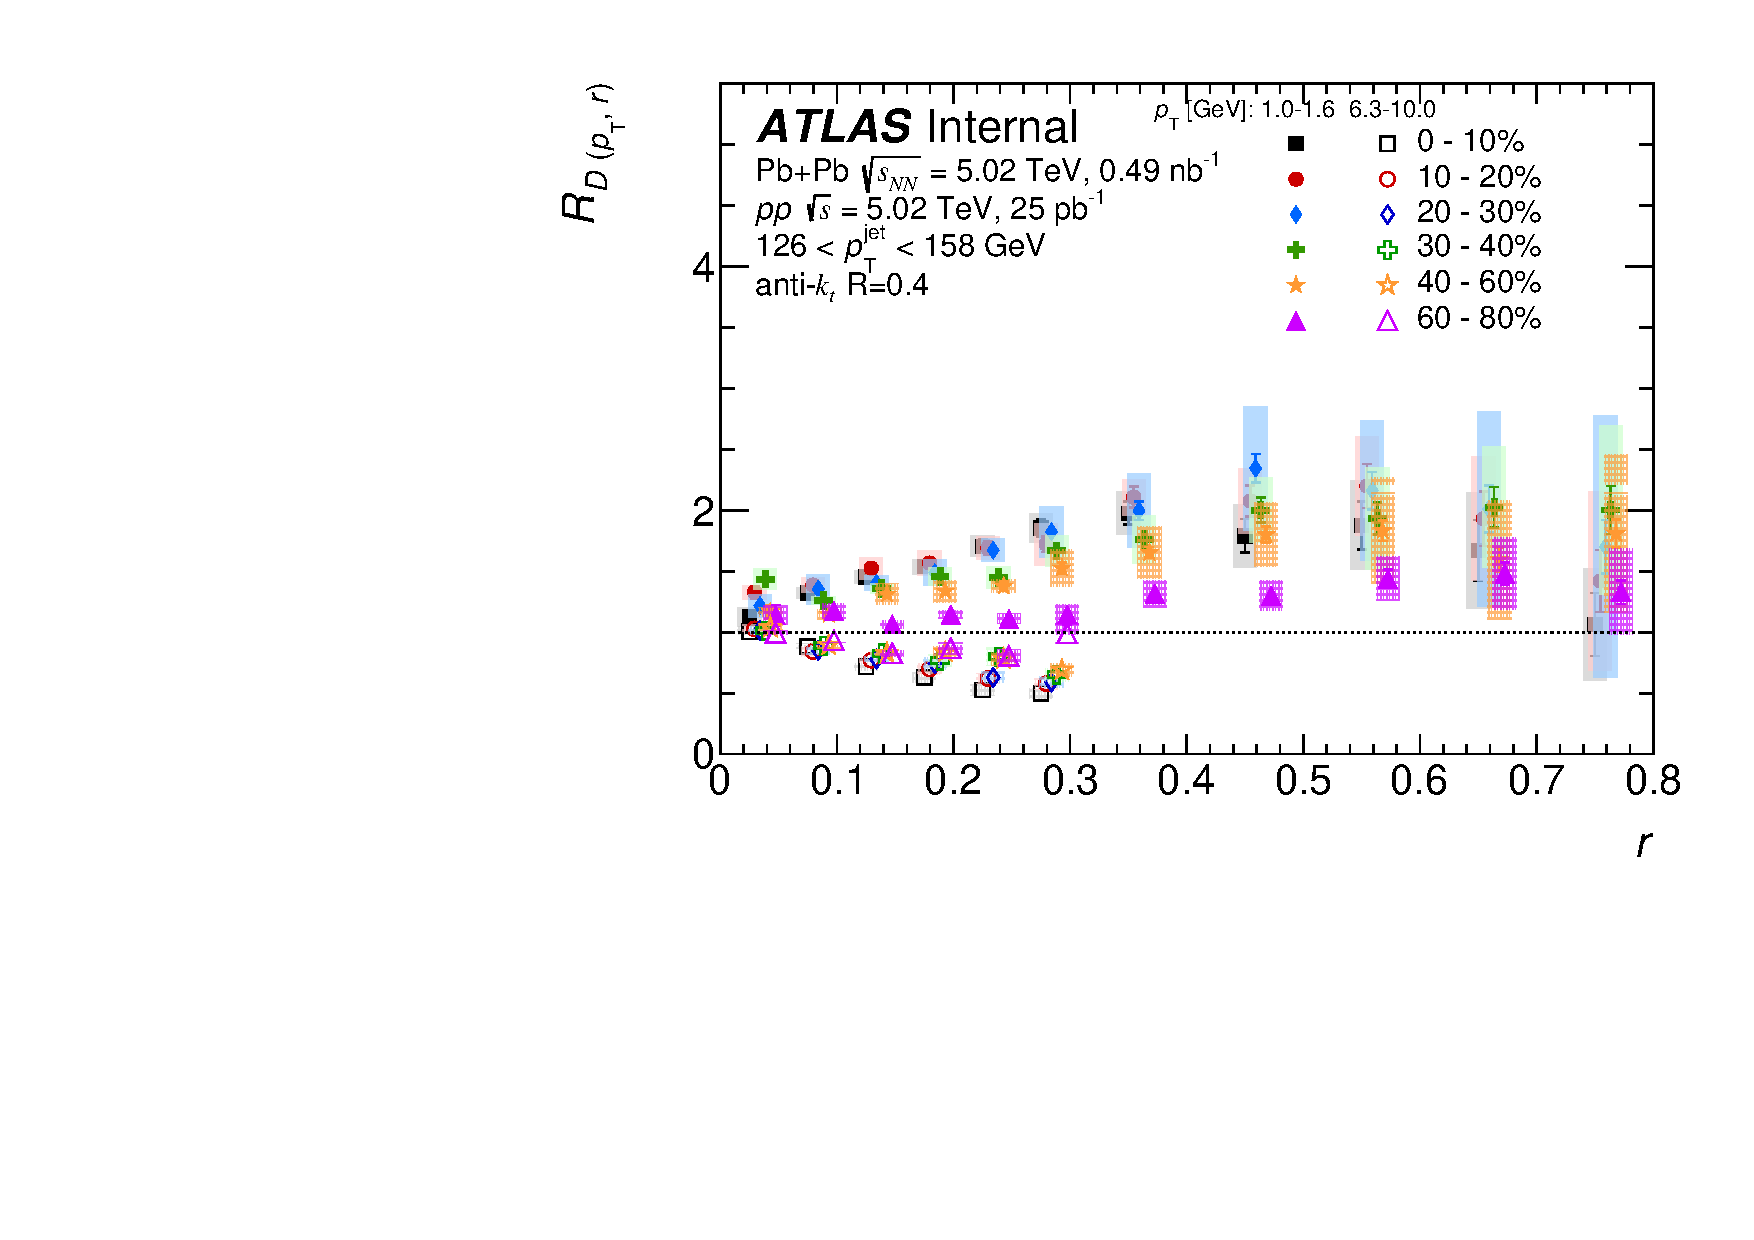
\includegraphics[width=0.5\textwidth]{figures/main/results/RDpT_dR_trk2_trk6_jet7.pdf} & 
%            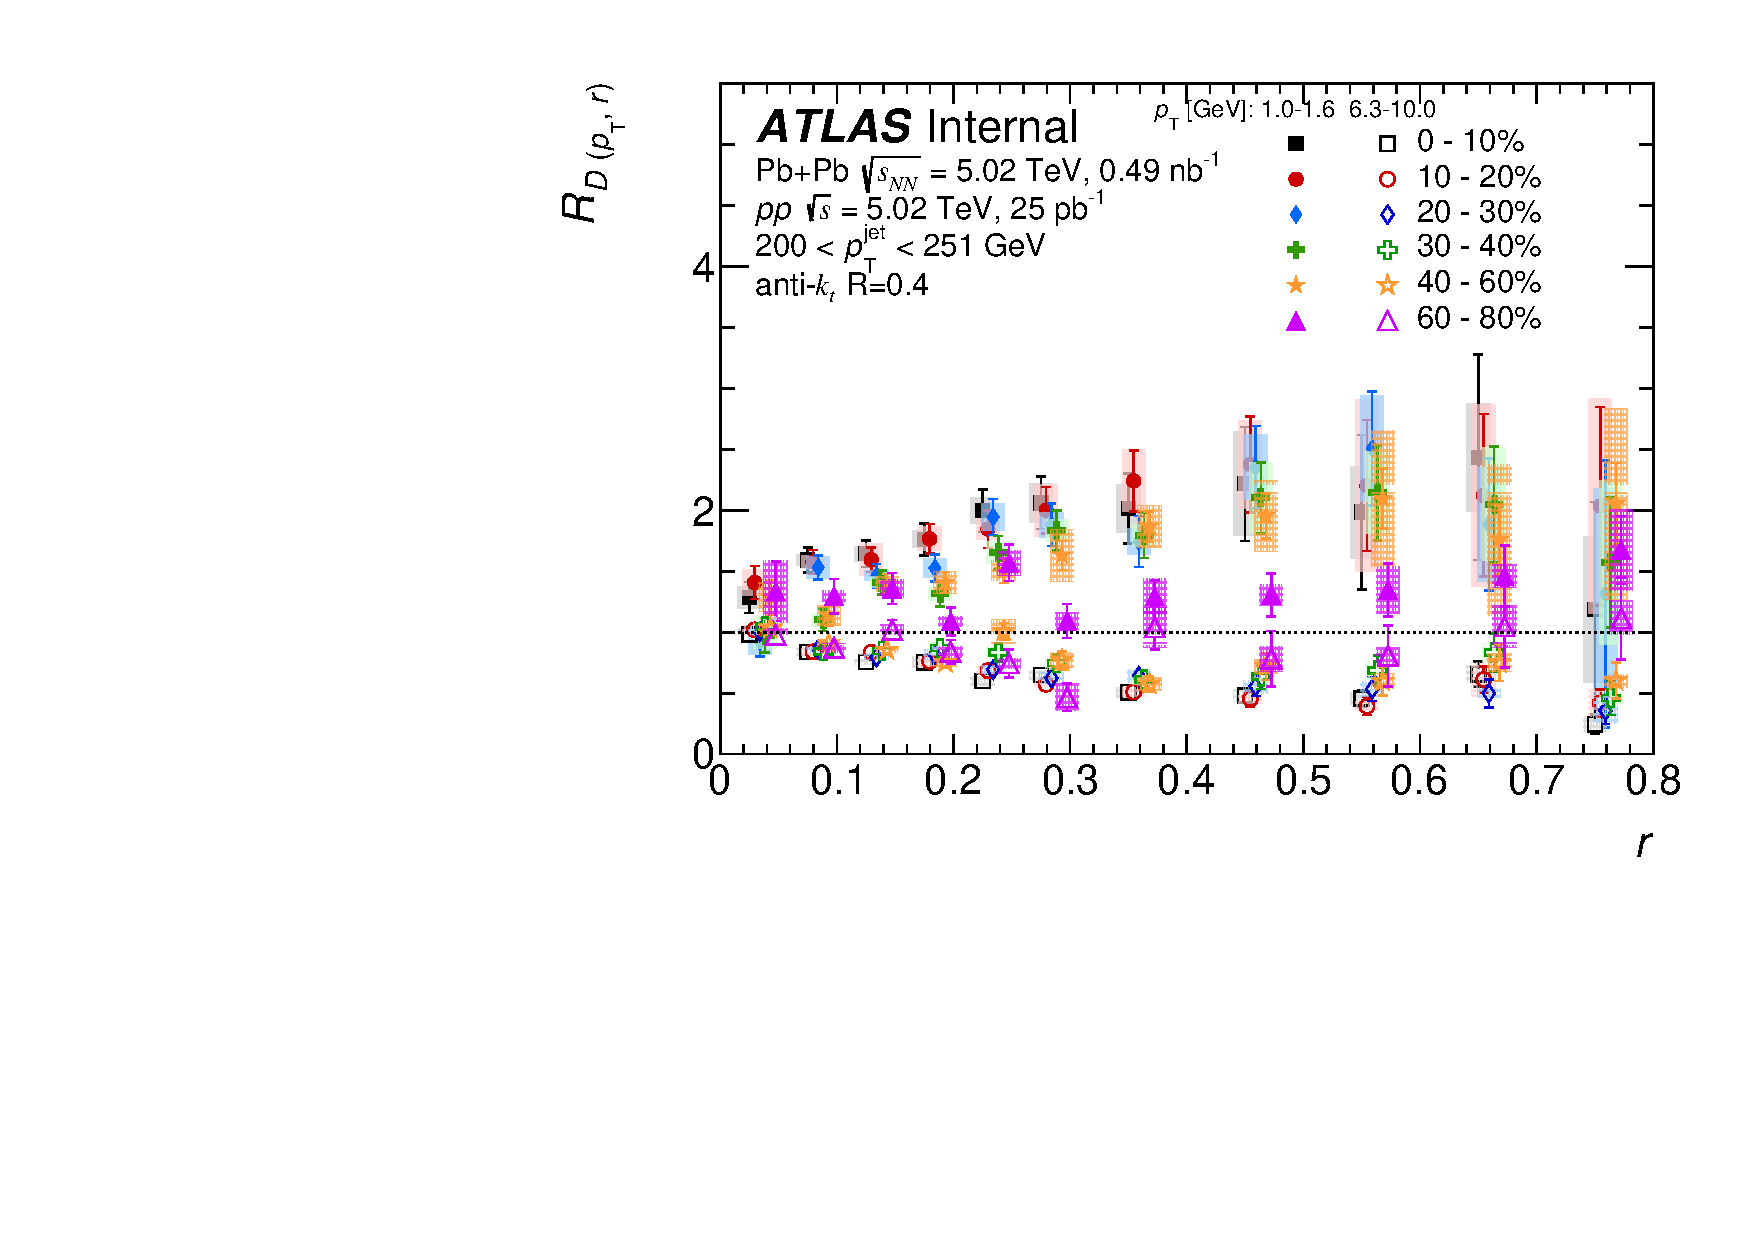
\includegraphics[width=0.5\textwidth]{figures/main/results/RDpT_dR_trk2_trk6_jet9.pdf} \\
            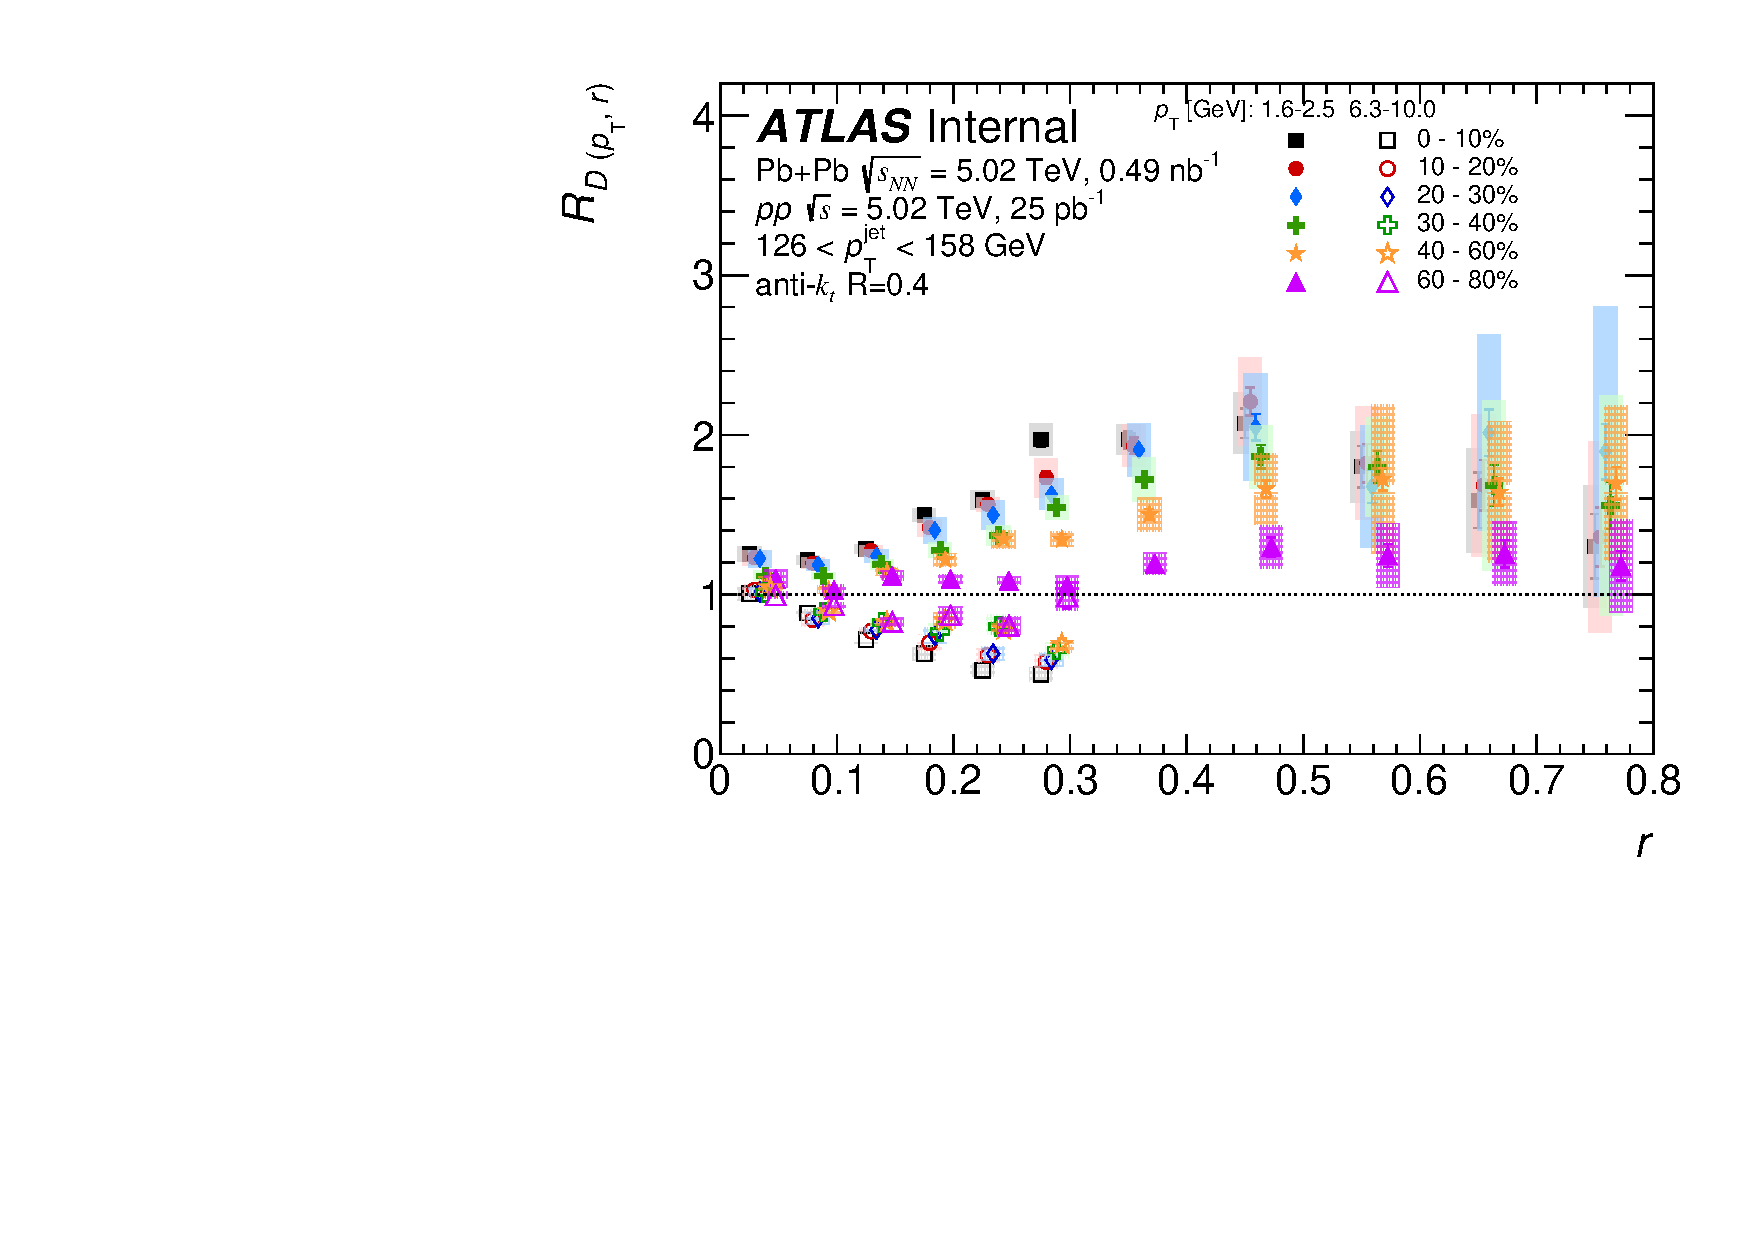
\includegraphics[width=0.5\textwidth]{figures/main/results/RDpT_dR_trk3_trk6_jet7.pdf} & 
            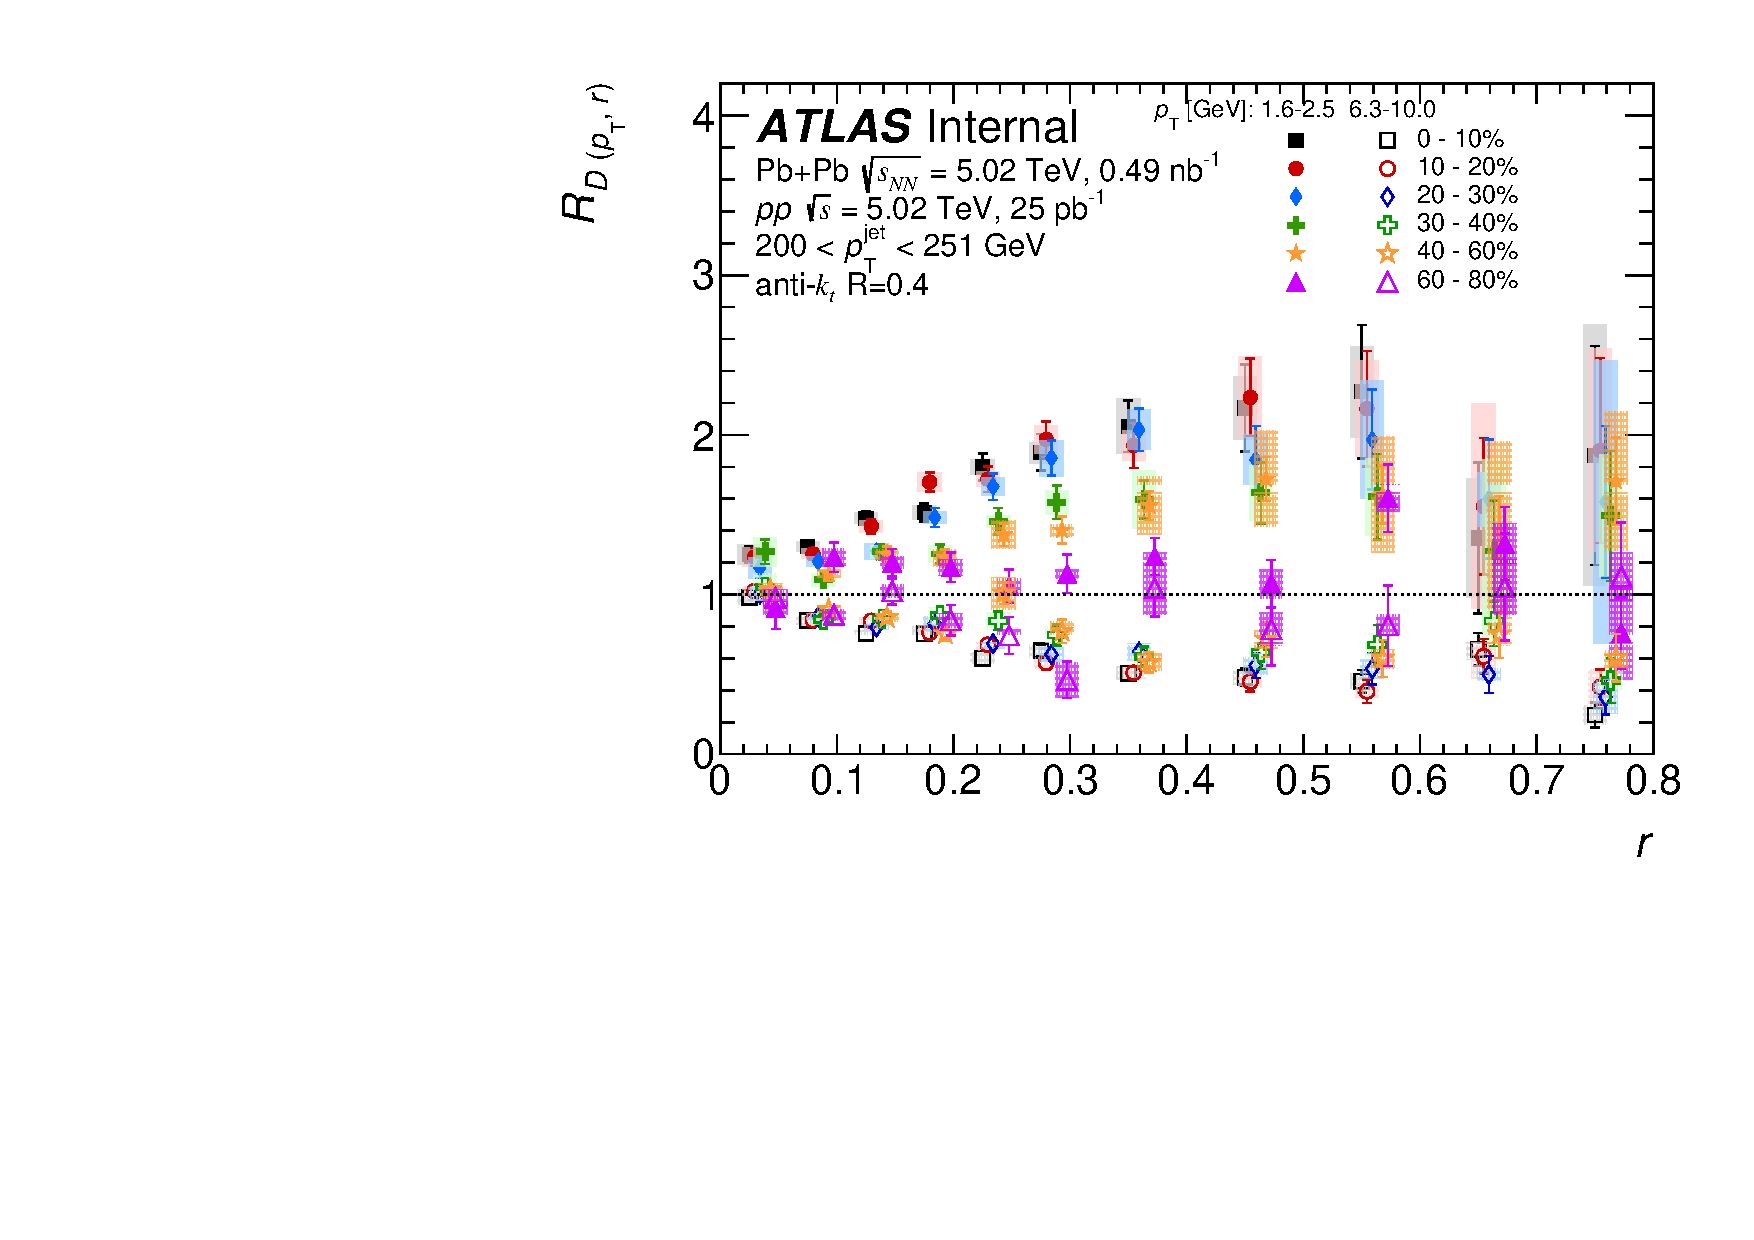
\includegraphics[width=0.5\textwidth]{figures/main/results/RDpT_dR_trk3_trk6_jet9.pdf} \\
      \end{tabular}
      }
   \caption{The \RDptr\ distributions for \ptjet\ of 126--158~\GeV\ and 200--251~\GeV\ as a function of angular distance $r$ for two \pt\ selections, 1.6--2.5~\GeV\ (closed symbols) and 6.3--10.0~\GeV\ (open symbols), and six centrality intervals.
The vertical bars on the data points indicate statistical uncertainties while the shaded boxes indicate systematic uncertainties.
The widths of the boxes are not indicative of the bin size and the points are shifted horizontally for better visibility.}
\label{fig:centdep}
\end{figure}
%%%%%%%%%%%%%

The centrality dependence of \RDptr\ for two charged-particle \pt\ intervals: 1.6--2.5~\GeV\ and \mbox{6.3--10.0~\GeV}, and two different \ptjet\ ranges: 126--158~\GeV\ and 200--251~\GeV, is presented in Figure~\ref{fig:centdep}.

For both \ptjet\ selections and  1.6--2.5~\GeV\ charged particles, the magnitude of the excess increases
with increasing collision centrality and \rvar\ for $\rvar < 0.3$.
 The magnitude of the excess is
approximately a factor of two in the most central collisions for $\rvar >$~0.3.
A continuous centrality dependent suppression of  yields of charged-particles with $6.3 < \pt < 10.0$ GeV is observed.
%%%%%%%%%%%%%%%%%
With the same \ptjet\ selections and 
charged-particles with 6.3~$ < \pt < $~10.0~\GeV a clear ordering in centrality is observed with
the most central collisions exhibiting the smallest \RDptr\ values.
%%%%%%%%%%%%%%%%%
The magnitude of the modifications decreases with decreasing collision centrality for both \pt\ 
intervals and \ptjet\ selections.

\begin{figure}[ht]
\centerline{
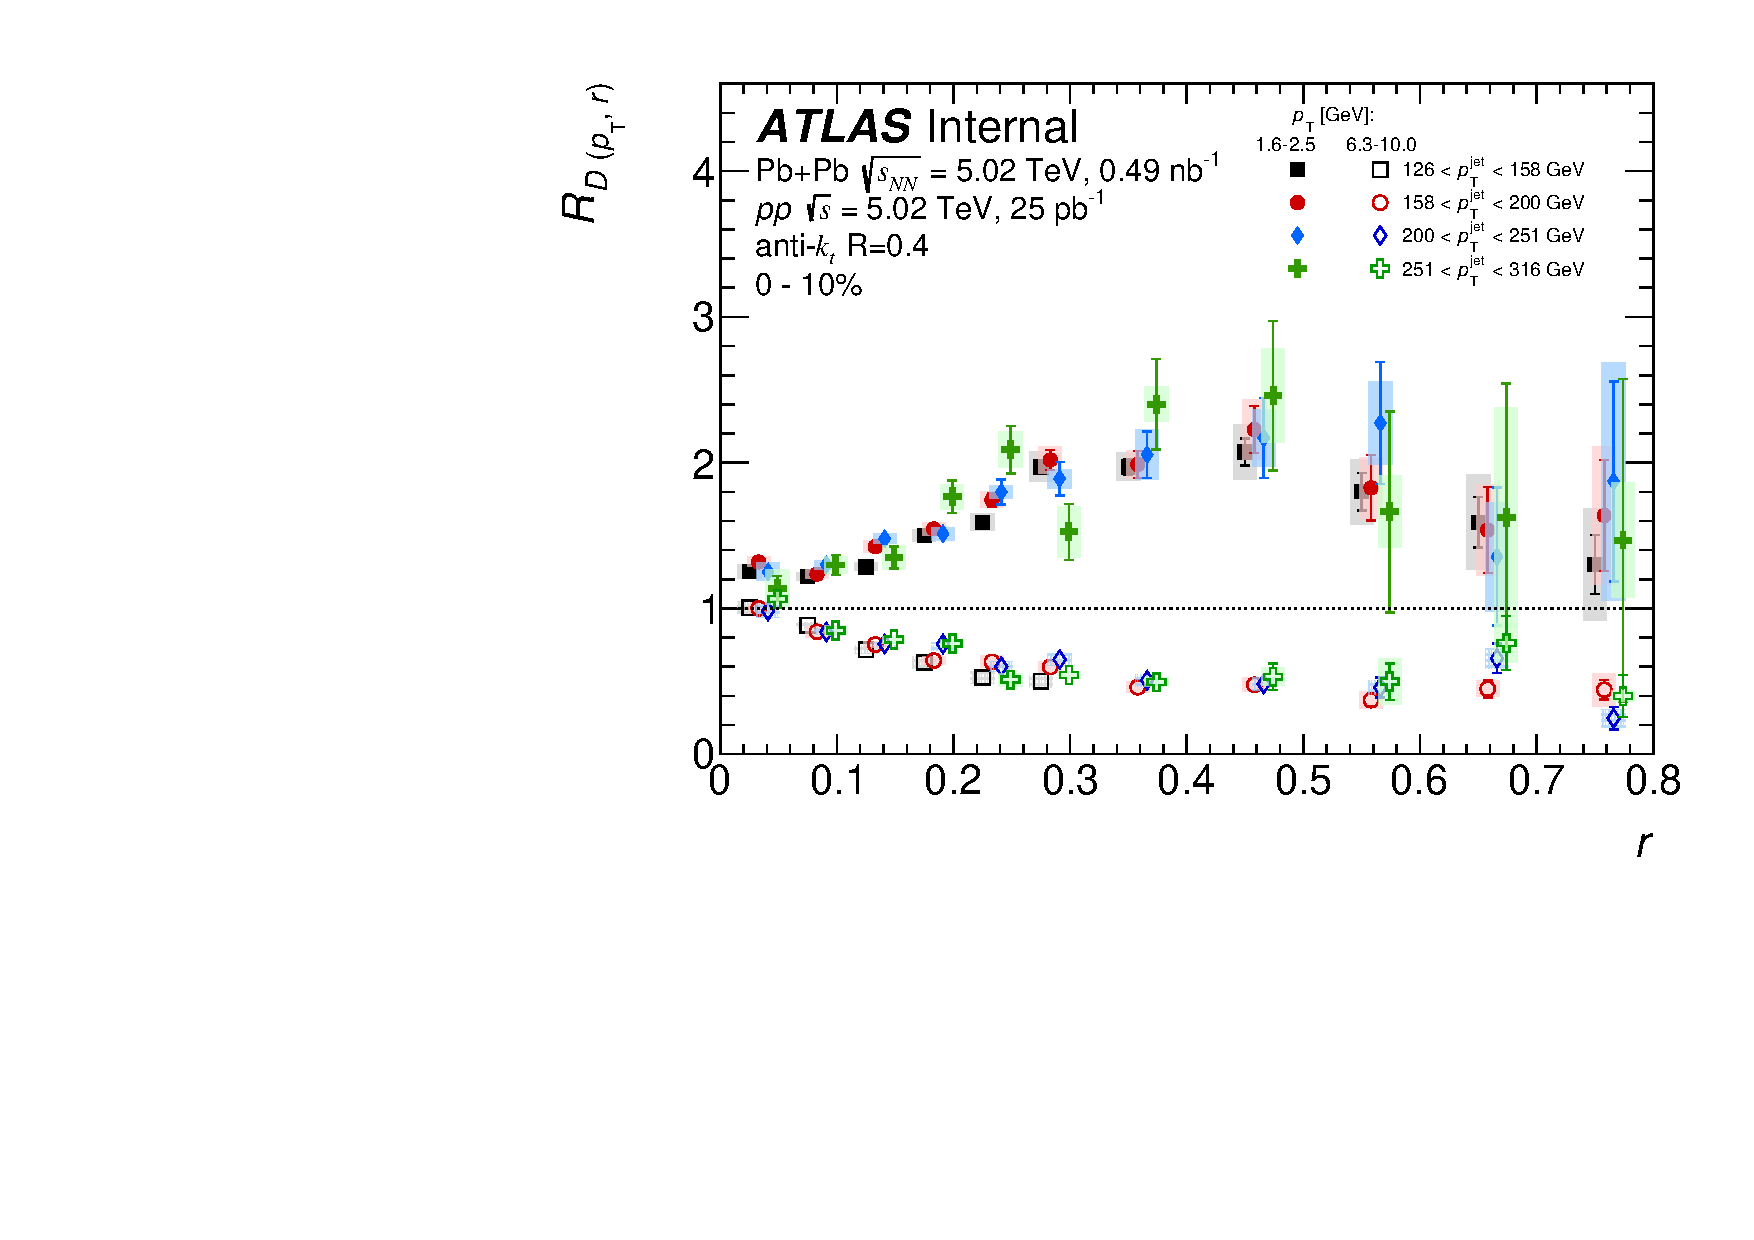
\includegraphics[width=0.8\textwidth]{figures/main/results/RDpT_dR_trk3_trk6_cent0.pdf} 
}
\caption{\RDptr\ as a function of \rvar\ for 0--10\% collisions for charged particles with 1.0~$< \pt <$~1.6~\GeV\
(closed symbols) and 6.3~$< \pt <$10.0~\GeV\ (open symbols) for different \ptjet\ selections.
The vertical bars on the data points indicate statistical uncertainties while the shaded boxes indicate systematic uncertainties.
The widths of the boxes are not indicative of the bin size and the points are shifted horizontally for better visibility.}
\label{fig:ptjetdep}
\end{figure}
%%%%%%%%%%%%%


%%%%%%%%%%%%%%%%%
%In order to directly explore the \ptjet\ dependence of \RDptr\, the values are overlaid for all four
%\ptjet\ selections measured here in Figure~\ref{fig:ptjetdep} for the 0--10\% most central collisions 
%and the same two charged-particle \pt\ selections as in Figure~\ref{fig:centdep}.
%%%%%%%%%%%%%%%%%
The \ptjet\ dependence of the \RDptr\ values is directly explored by overlaying 
\ptjet\ selections in Figure~\ref{fig:ptjetdep}.
These distributions are for the 0--10\% 
most central collisions, for the same two charged-particle \pt\ selections shown in Figure~\ref{fig:centdep}.

  A trend of increasing \RDptr\ with increasing \ptjet\ is observed for $r < 0.25$ for low 
\pt\ charged particles; at larger \rvar\ values there is no significant dependence of \RDptr\ on \ptjet.

Furthermore, for the higher-\pt\ charged particles, no significant dependence on \ptjet\ is observed.



\begin{figure}
\centering{
\begin{tabular}{cc}
	 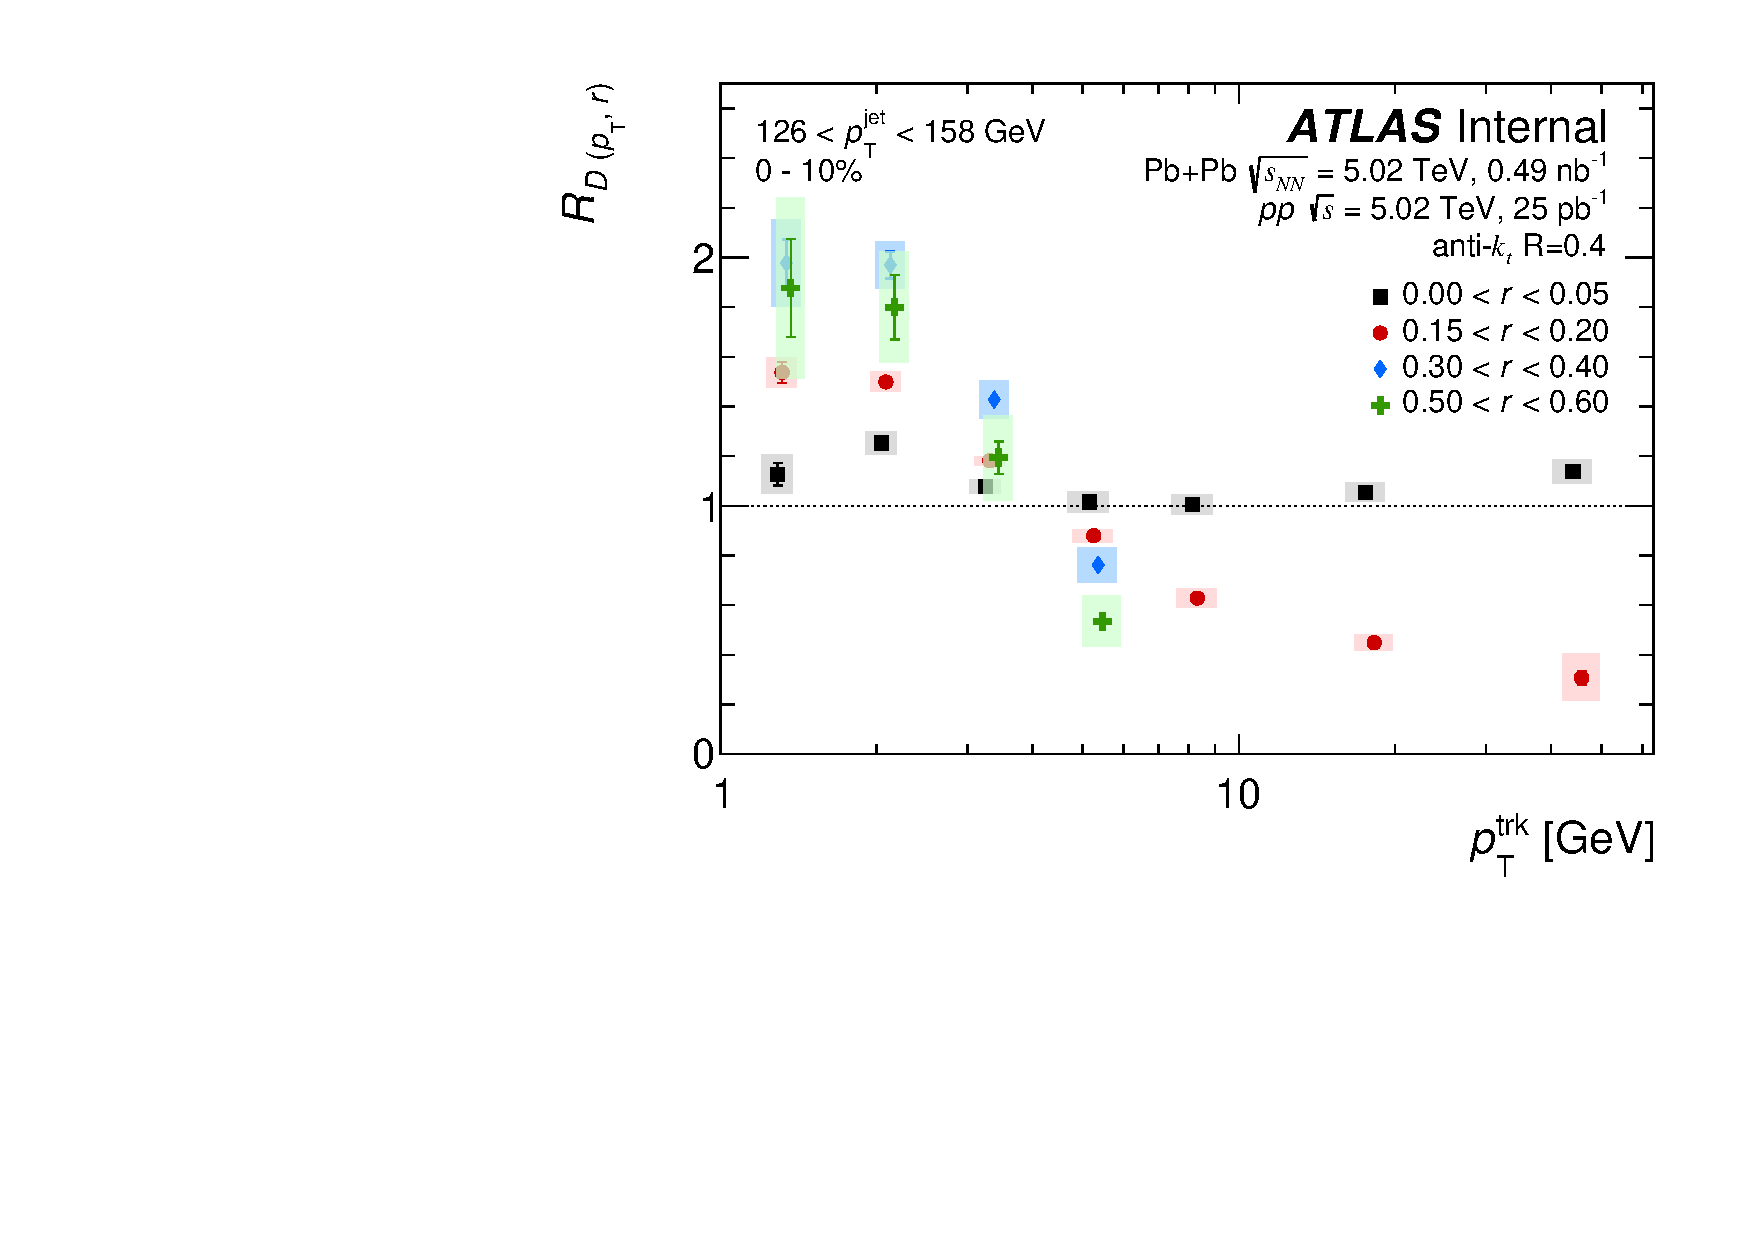
\includegraphics[width=0.5\textwidth]{figures/main/results/RDpT_trkpt_jet7_cent0} &
	 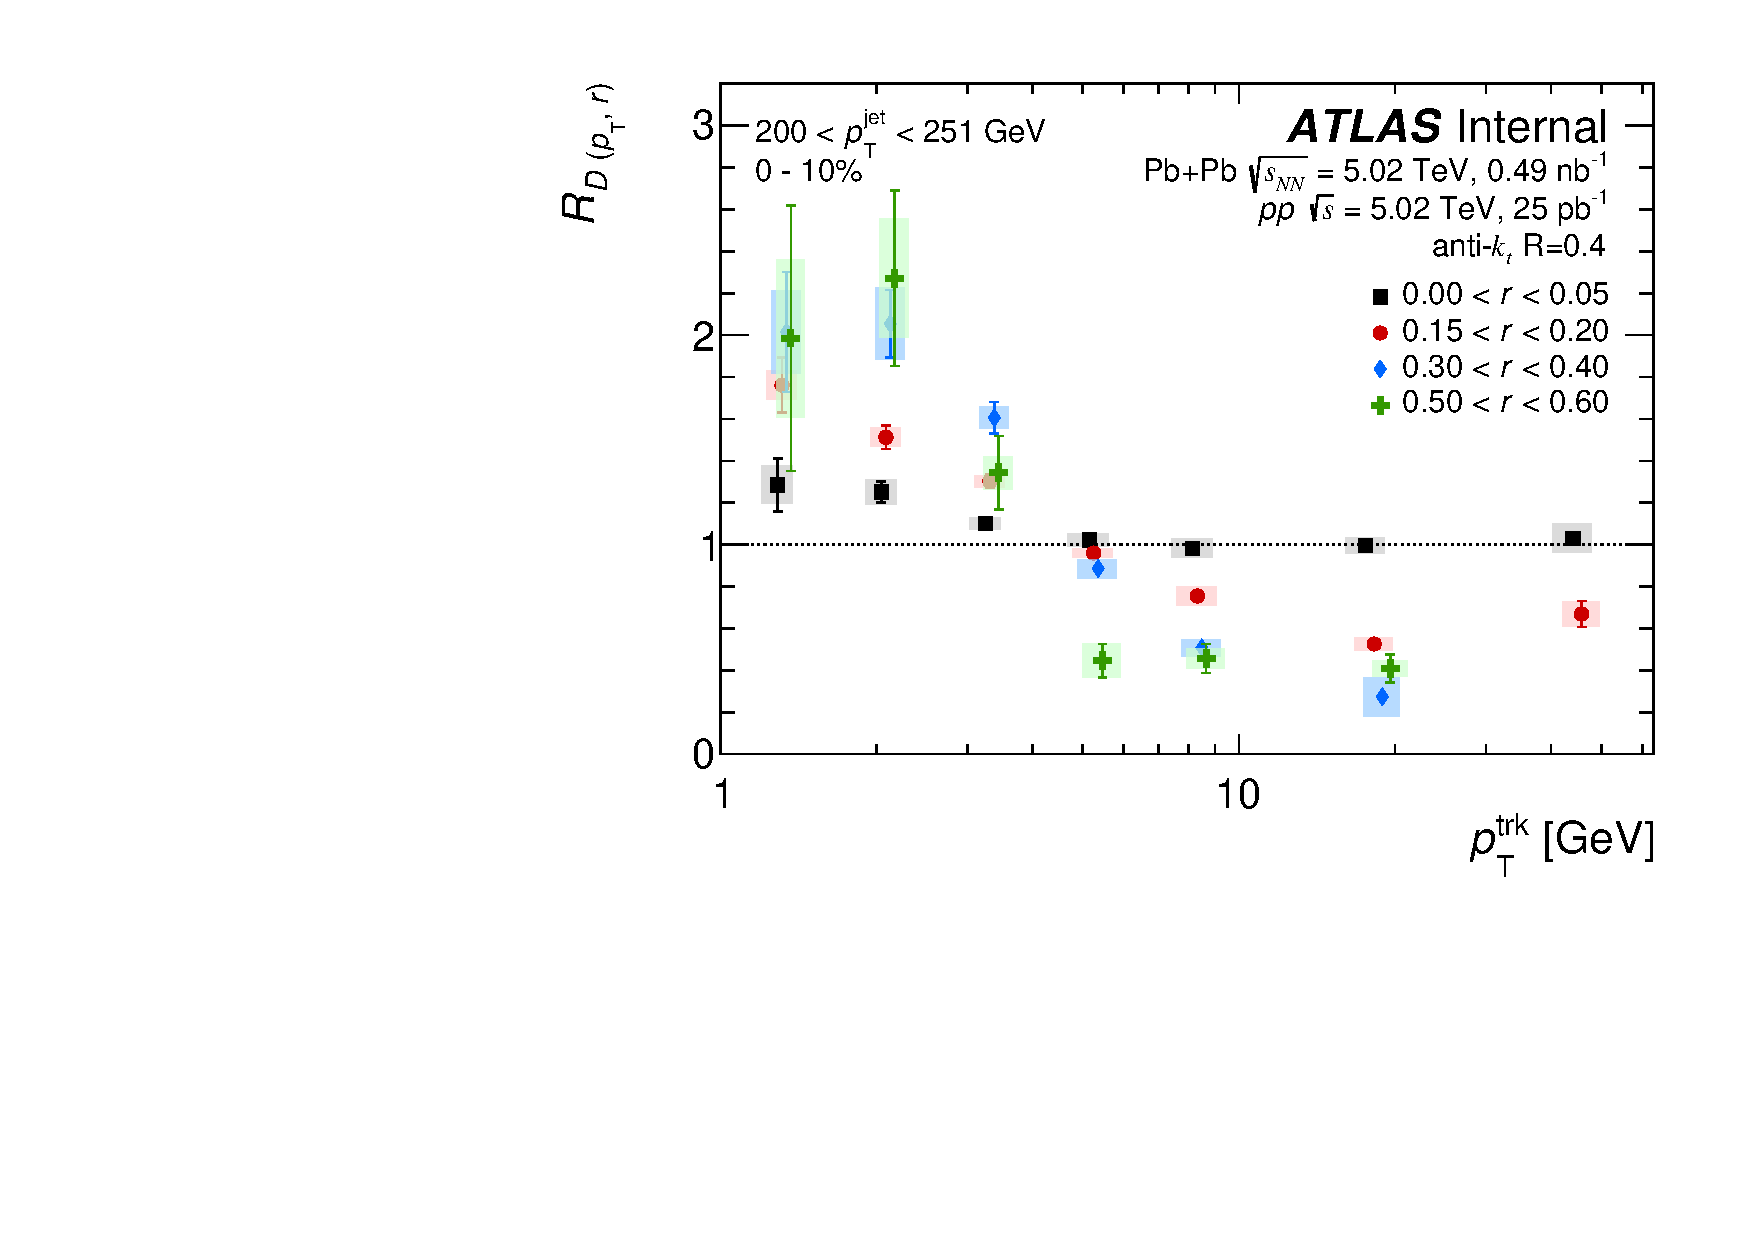
\includegraphics[width=0.5\textwidth]{figures/main/results/RDpT_trkpt_jet9_cent0} \\
	 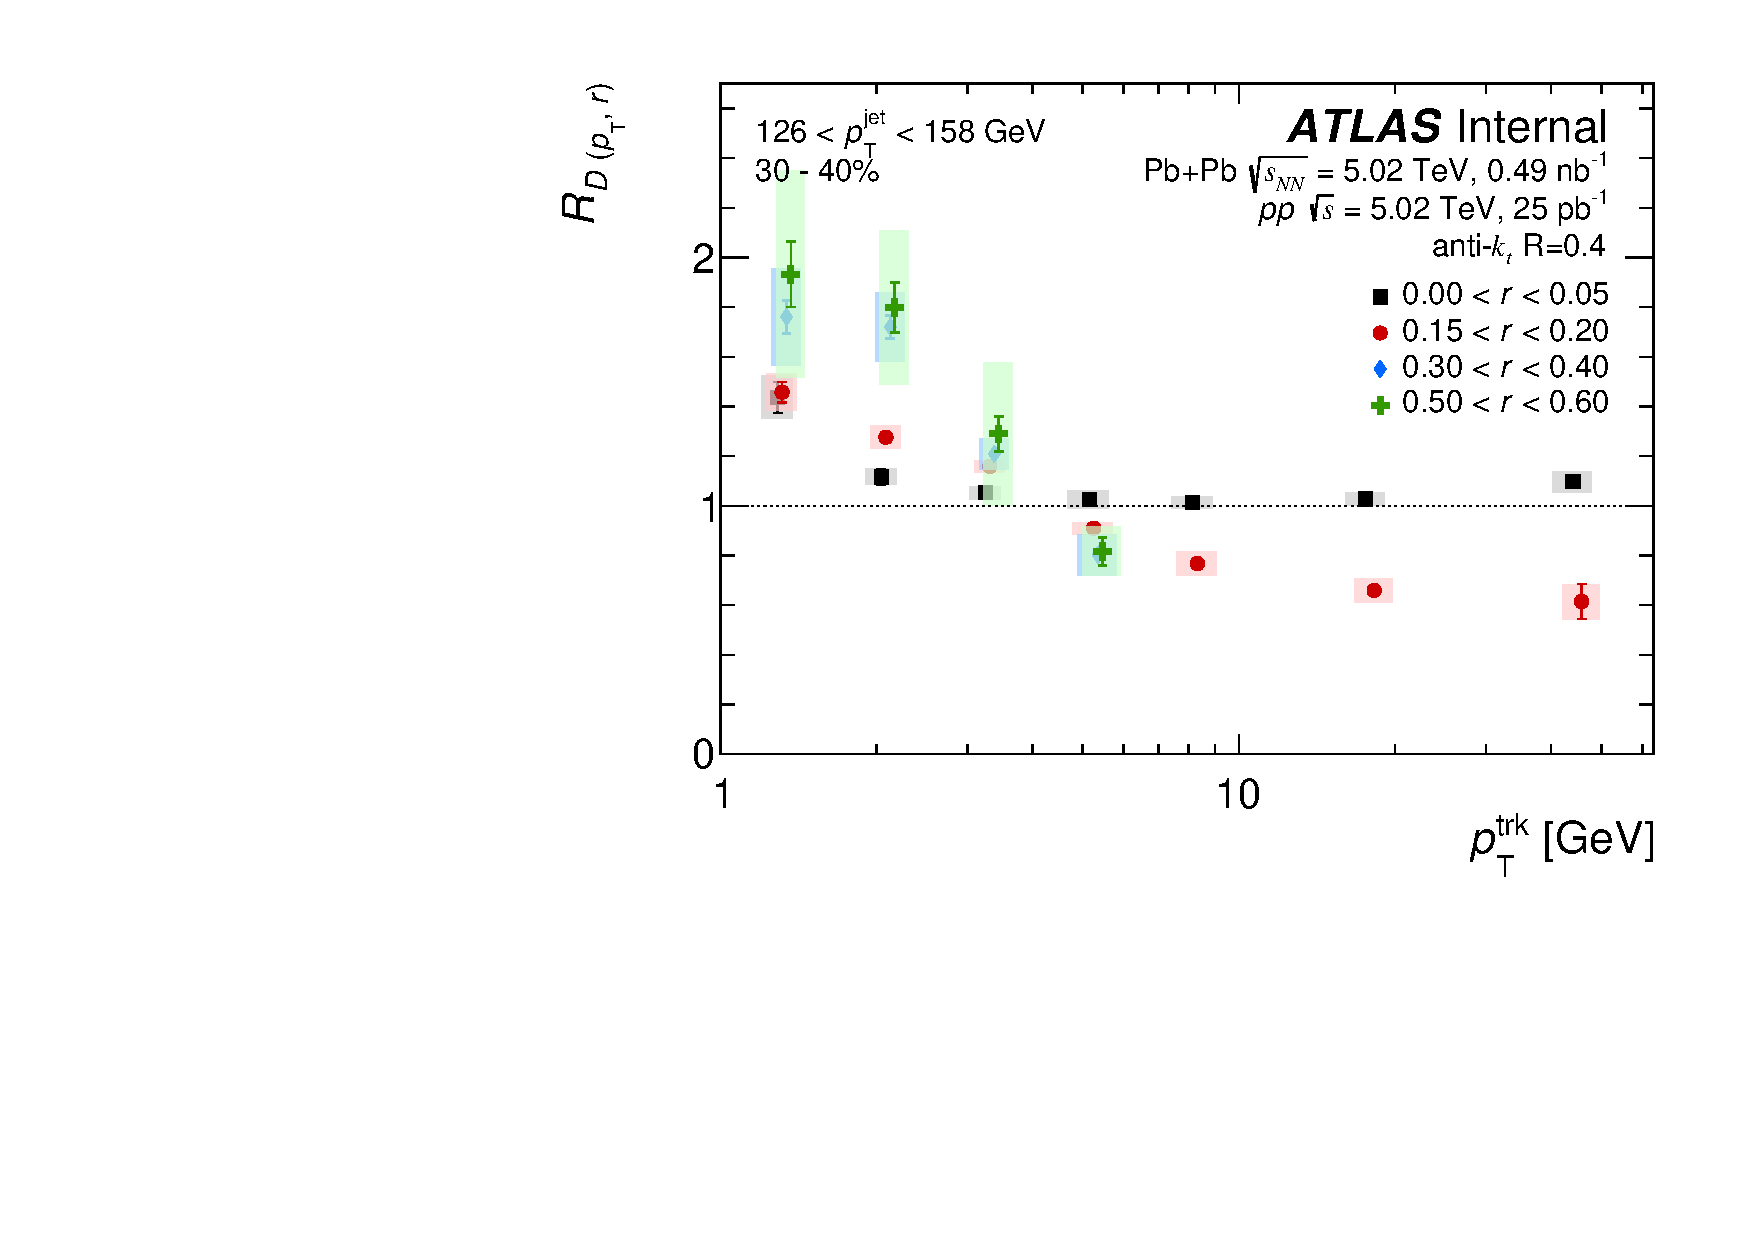
\includegraphics[width=0.5\textwidth]{figures/main/results/RDpT_trkpt_jet7_cent3} &
	 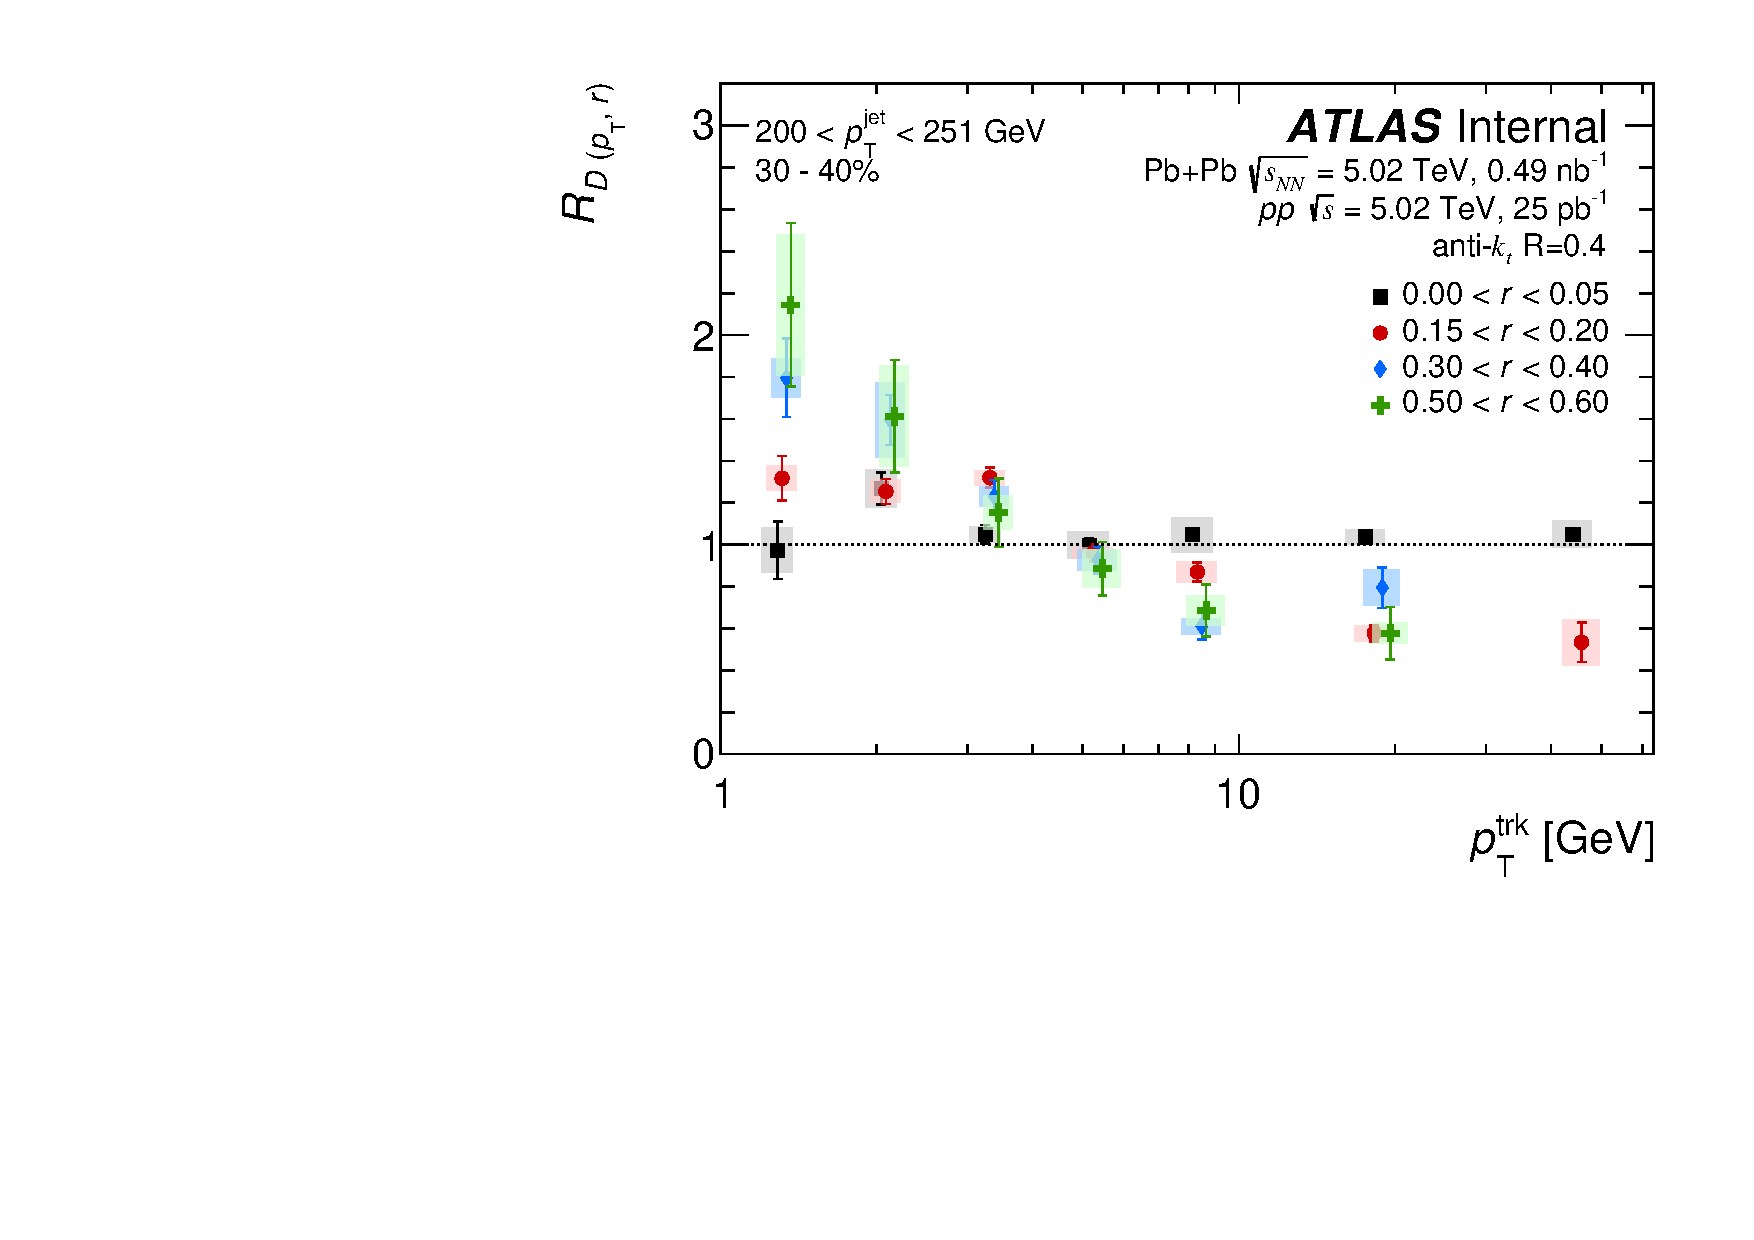
\includegraphics[width=0.5\textwidth]{figures/main/results/RDpT_trkpt_jet9_cent3} \\
	 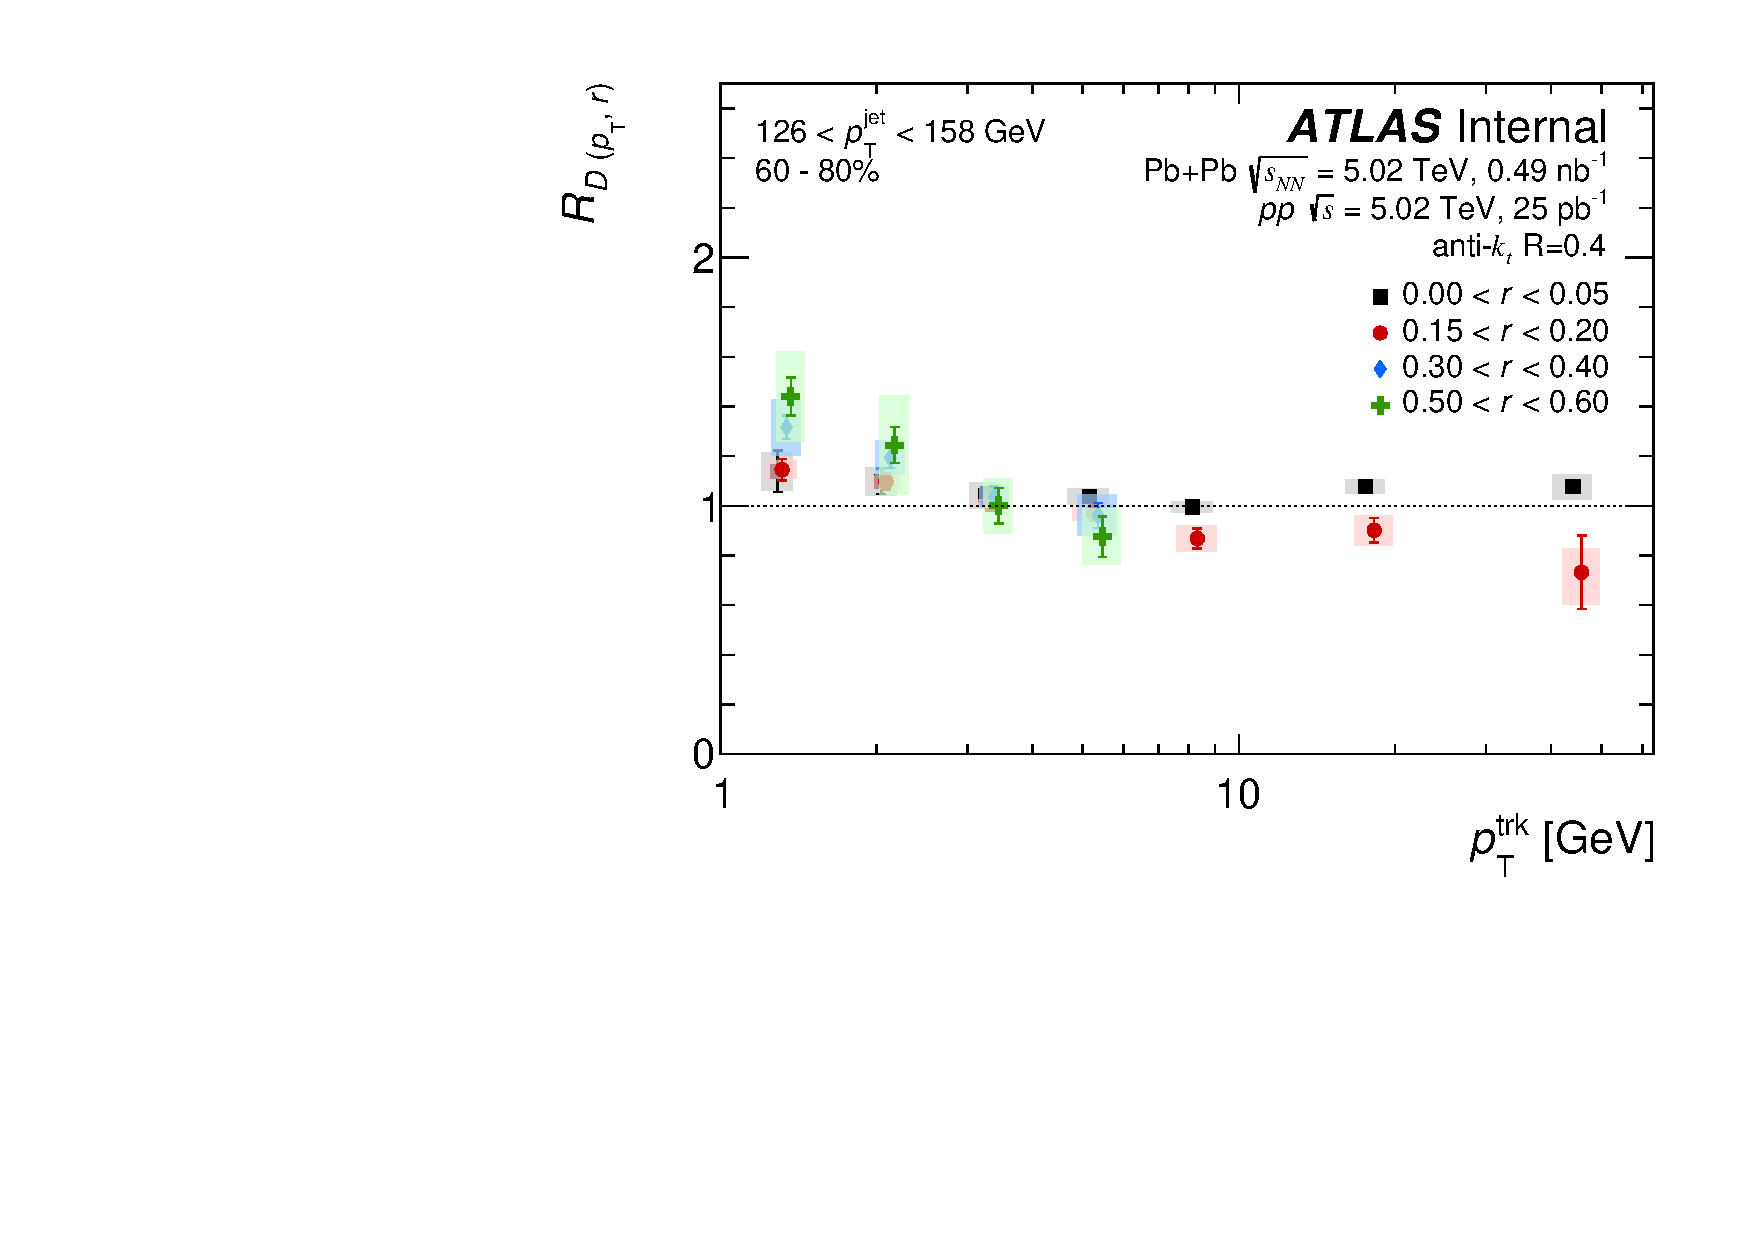
\includegraphics[width=0.5\textwidth]{figures/main/results/RDpT_trkpt_jet7_cent5} &
	 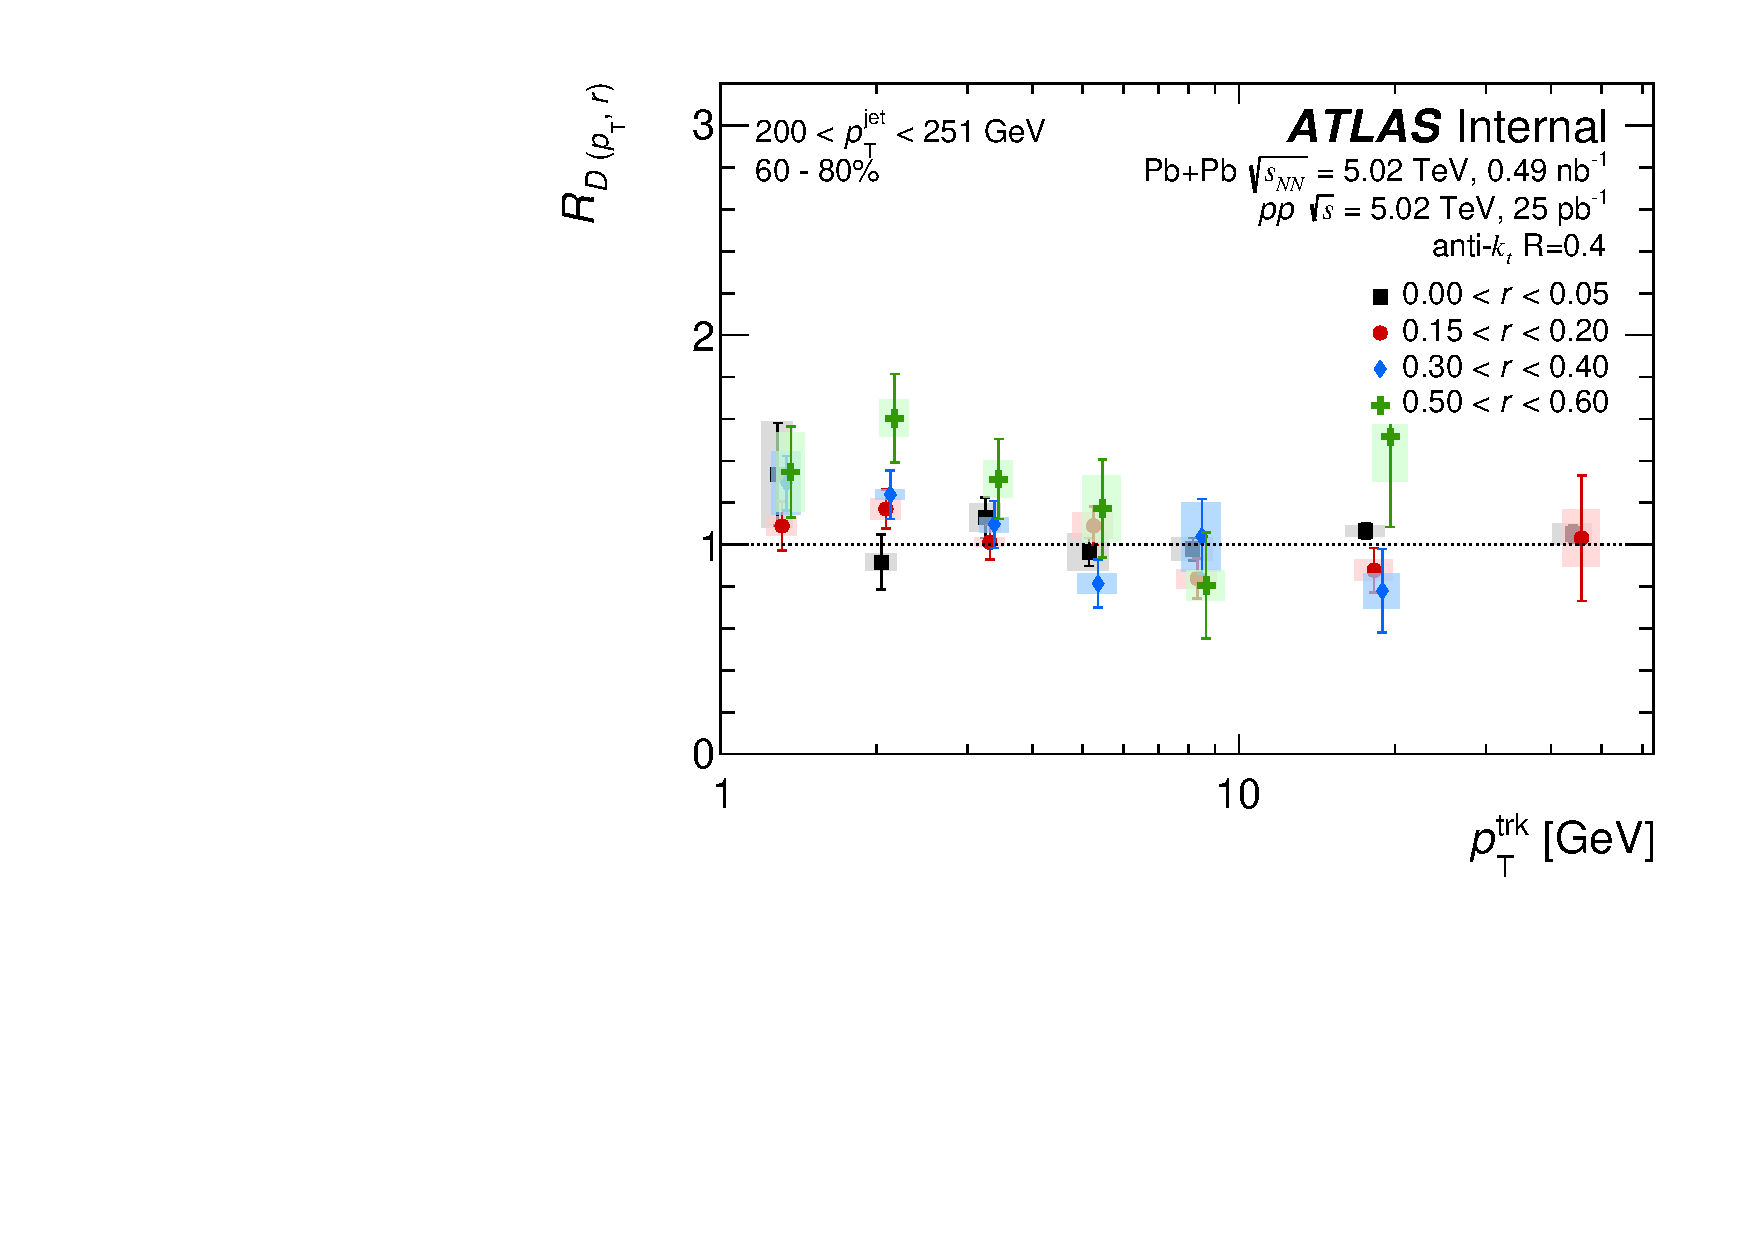
\includegraphics[width=0.5\textwidth]{figures/main/results/RDpT_trkpt_jet9_cent5} \\
\end{tabular} }
   \caption{\RDptr\ as a function of \pt\ in  0--10\% (top), 30--40\% (middle), and 60--80\% (bottom) \PbPb\ collisions to \pp\ collisions for two different \ptjet\ selections: 126--158~\GeV\ (left) and 200--251~\GeV\ (right).
The different colors indicate different angular distances from the jet axis.
The vertical bars on the data points indicate statistical uncertainties while the shaded boxes indicate systematic uncertainties.
The widths of the boxes are not indicative of the bin size and the points are shifted horizontally for better visibility.}
      \label{fig:pttrkdep}
\end{figure}


%%pt track dependence
In Figure~\ref{fig:rdptr}, it was shown that for central and mid-central collisions, there is an enhancement of
charged particles with $\pt <$~4.0~\GeV\ and a suppression of charged particles with $\pt >$~4.0~\GeV.
 In
Figure~\ref{fig:pttrkdep} 
the \pt\ dependance for selections in \rvar\ is directly investigated for 0--10\%, 30--40\% and 60--80\% central 
collisions for 126--158 and 200--251~\GeV\ jets.
Interestingly, at all measured \pt, there is no significant suppression of the yields in \pbpb\ collisions
for $\rvar < 0.05$.
 For larger \rvar\ values the yields are enhanced for charged-particles with $\pt <$~4~\GeV\ and 
suppressed for higher \pt\ charged-particles in both the 0--10\% and 30--40\% centrality selections and both \ptjet\ 
ranges presented here.
 The magnitude of the enhancement increases for decreasing \pt\ at low \pt and increases
with increasing \pt at high \pt, until about 10~\GeV, after which the suppression remains approximately constant.
At fixed \pt\ the magnitude of the deviation from unity is largest for 0.3$< \rvar <$~0.4 and 0.5$< \rvar <$~0.6.
In the 60--80\% central collisions, the same trend remains true (but with smaller magnitude 
modifications) for \mbox{$126 < \ptjet < 158$ GeV}; for the higher \ptjet\ selection the larger uncertainties 
do not allow a clear conclusion to be drawn for peripheral collisions.

One possible explanation of the modification of the 
jet fragmentation in this kinematic range~\cite{PhysRevC.98.024908} is the larger expected energy loss
of gluon-initiated jets leading to a relative enhancement of quark jets in \pbpb\ collisions compared
to \pp\ collisions at a given \ptjet\ value~\cite{Spousta:2015fca}.
Since gluon jets have a broader distribution of particle transverse momentum with respect to the jet direction compared to quark-initiated jets \cite{OPAL:1995ab}
 , such an effect could potentially describe the narrowing of particle distribution around the jet direction for particles with $\pt >$~4.0~\GeV\
observed here, though no calculations of this are available.

%%%%%%%%%%%%%%%%%
%\begin{figure}
%\centering{
%\begin{tabular}{cc}
%	 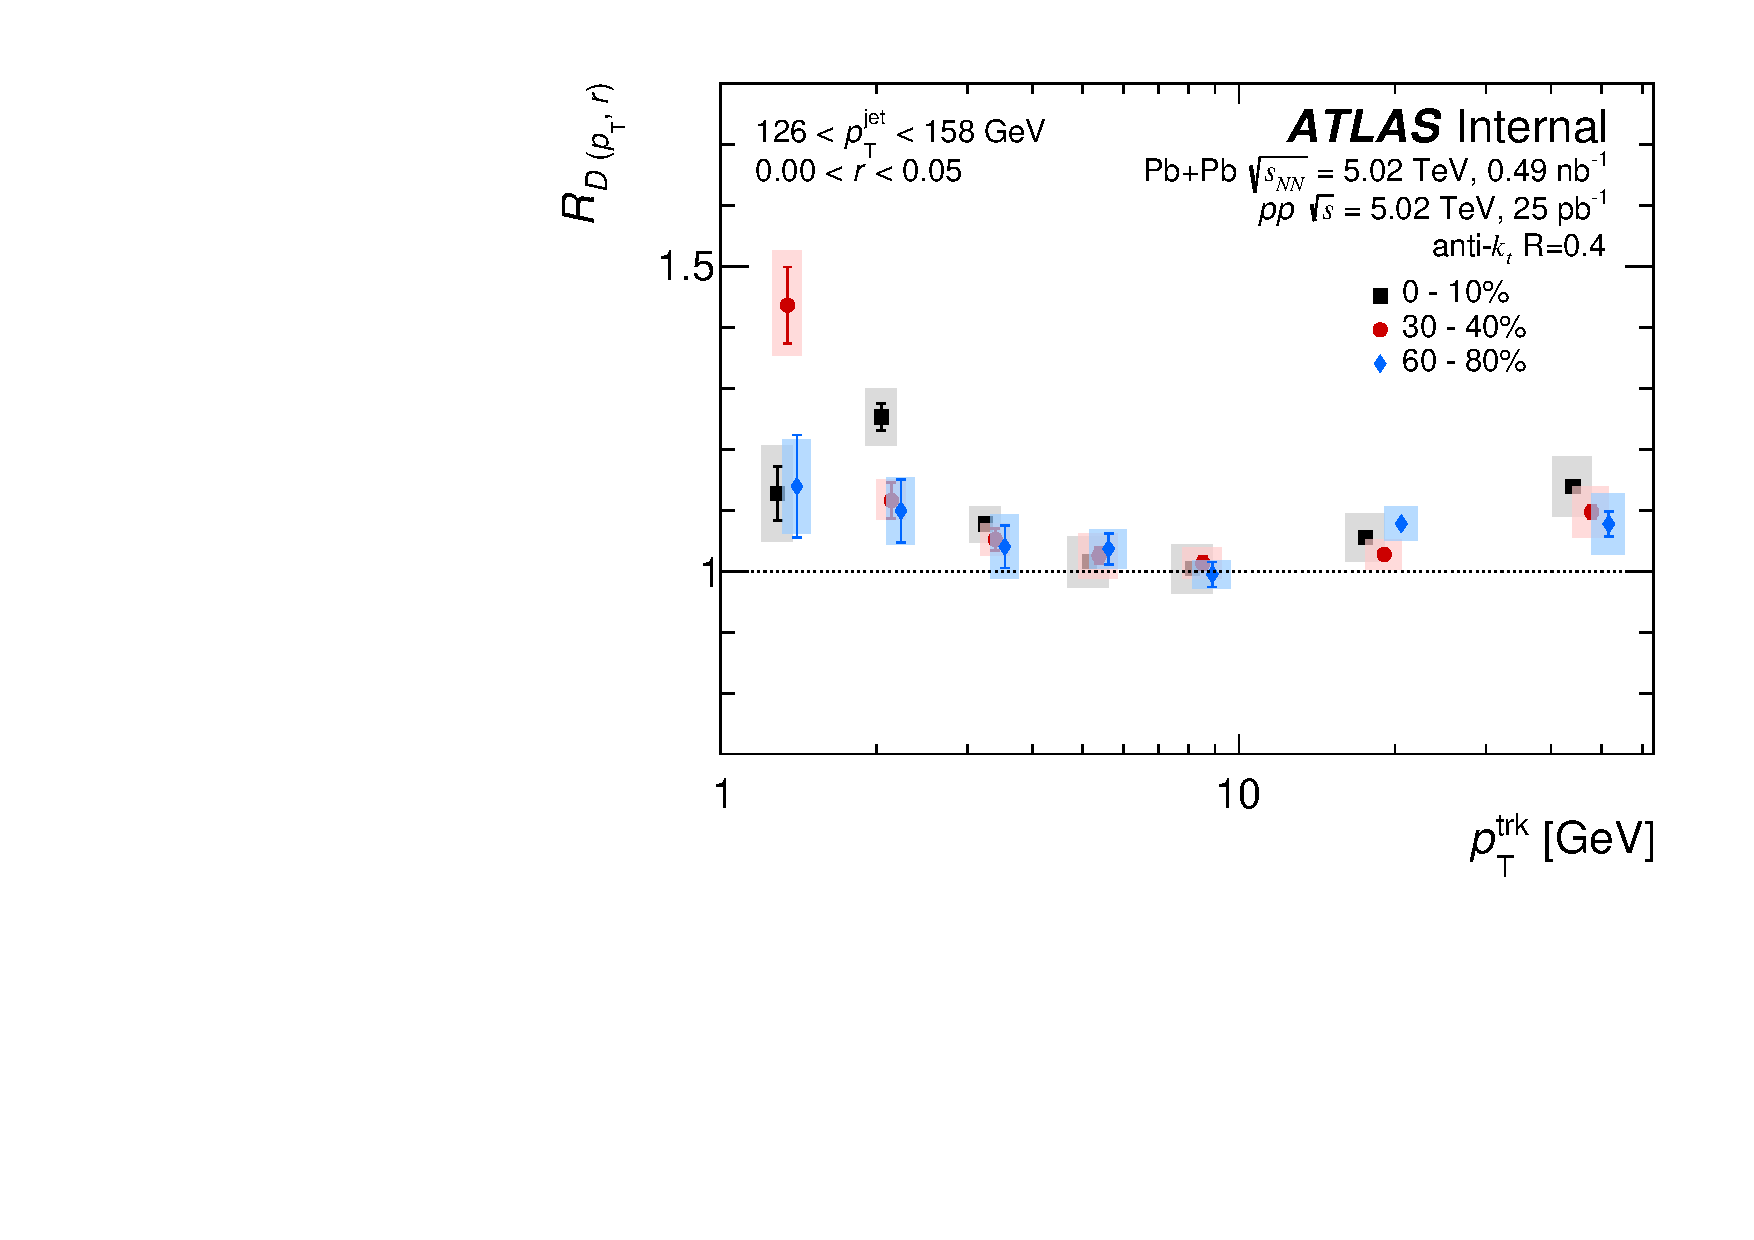
\includegraphics[width=0.5\textwidth]{figures/main/results/RDpT_trkpt_jet7_dR0} &
%	 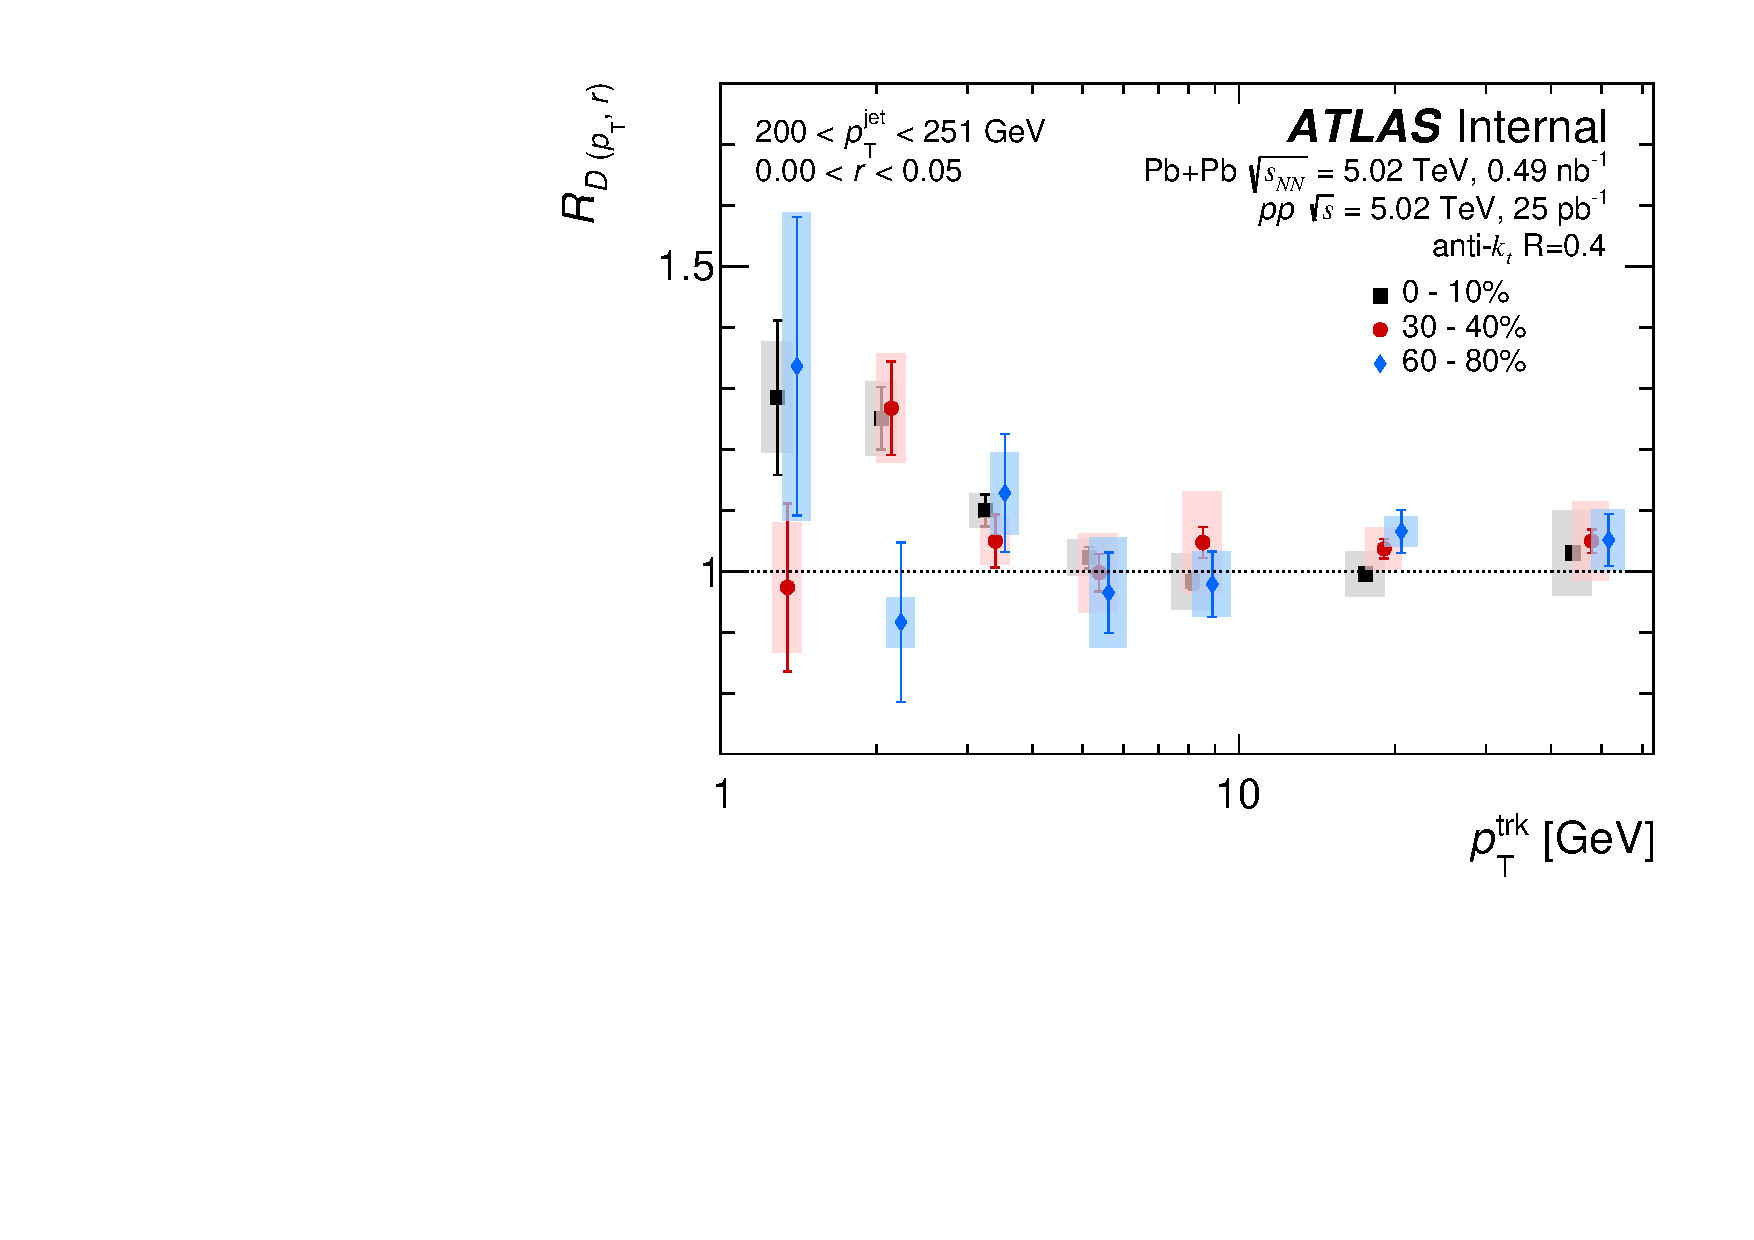
\includegraphics[width=0.5\textwidth]{figures/main/results/RDpT_trkpt_jet9_dR0} \\
%	 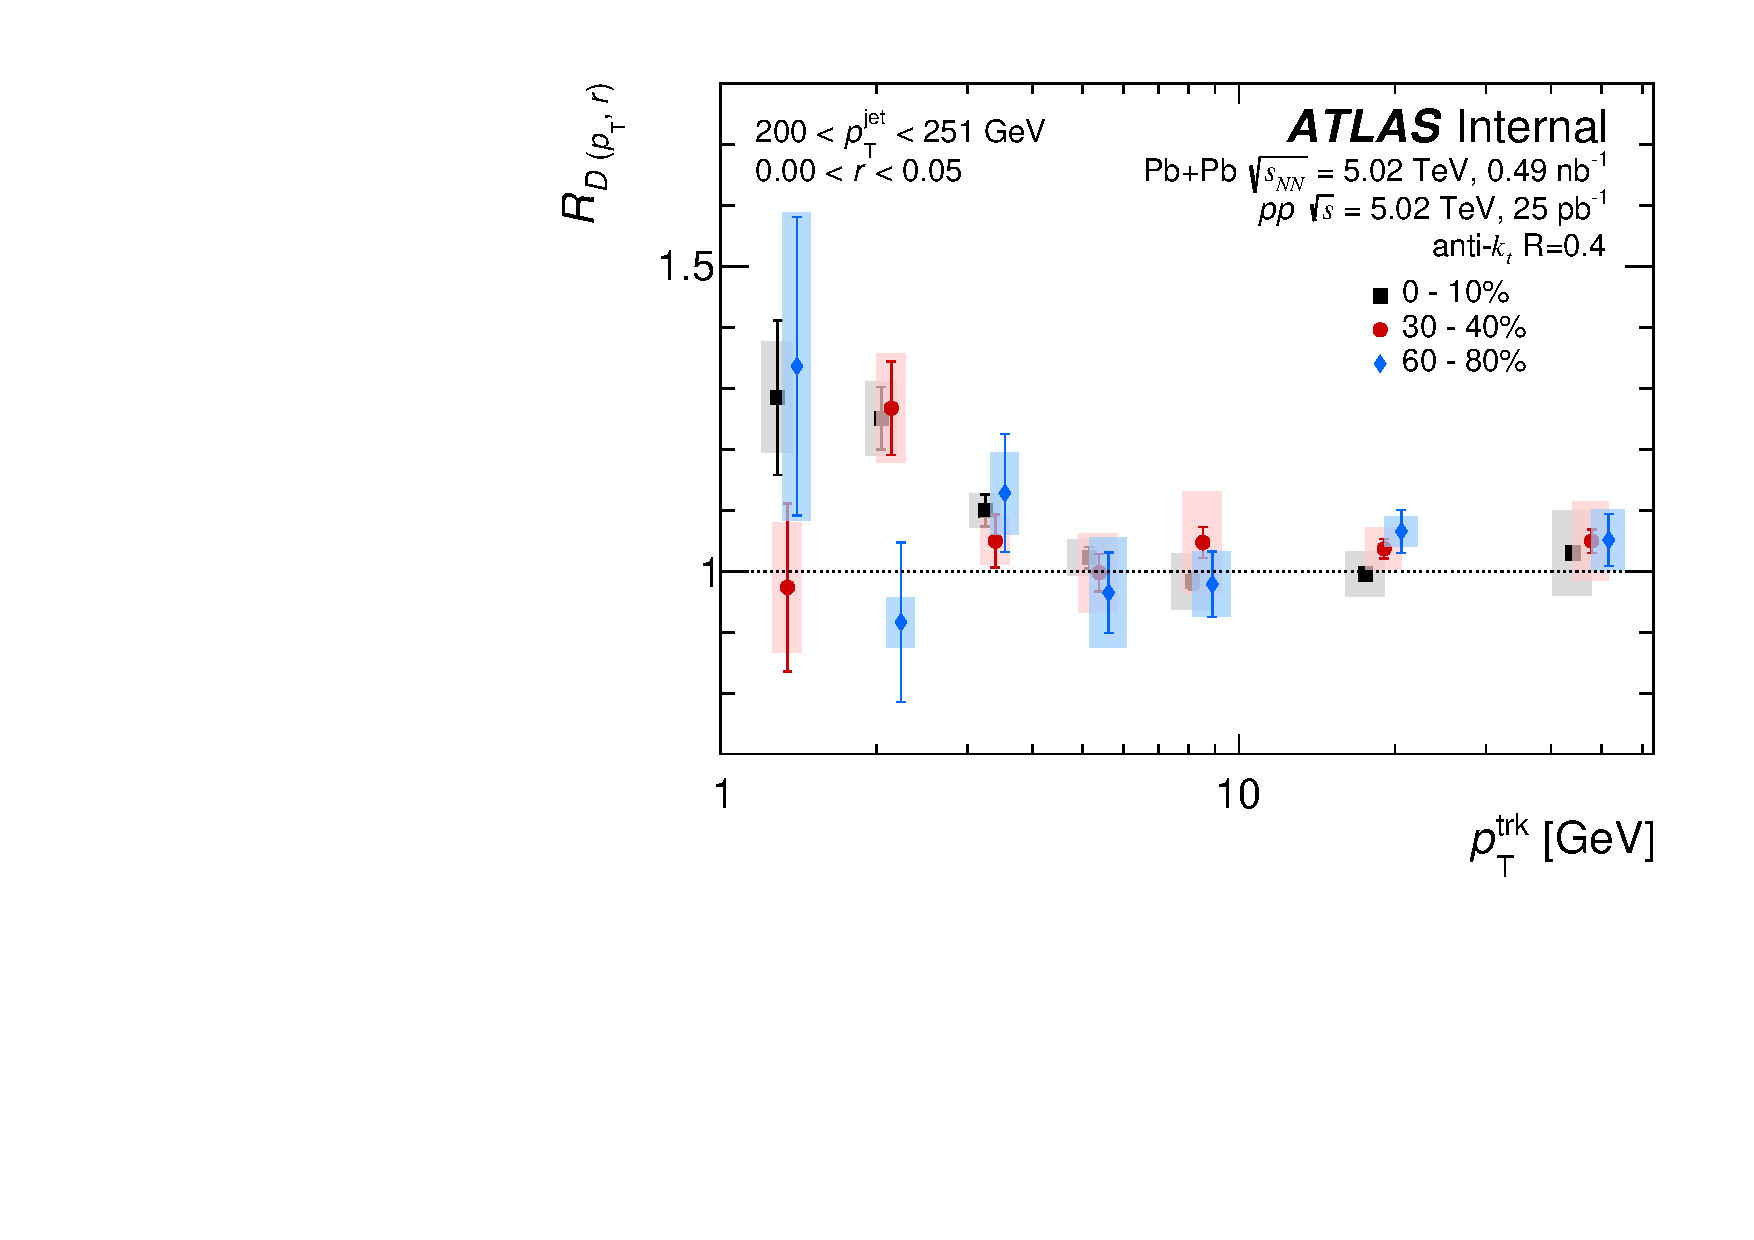
\includegraphics[width=0.5\textwidth]{figures/main/results/RDpT_trkpt_jet9_dR0} &
%	 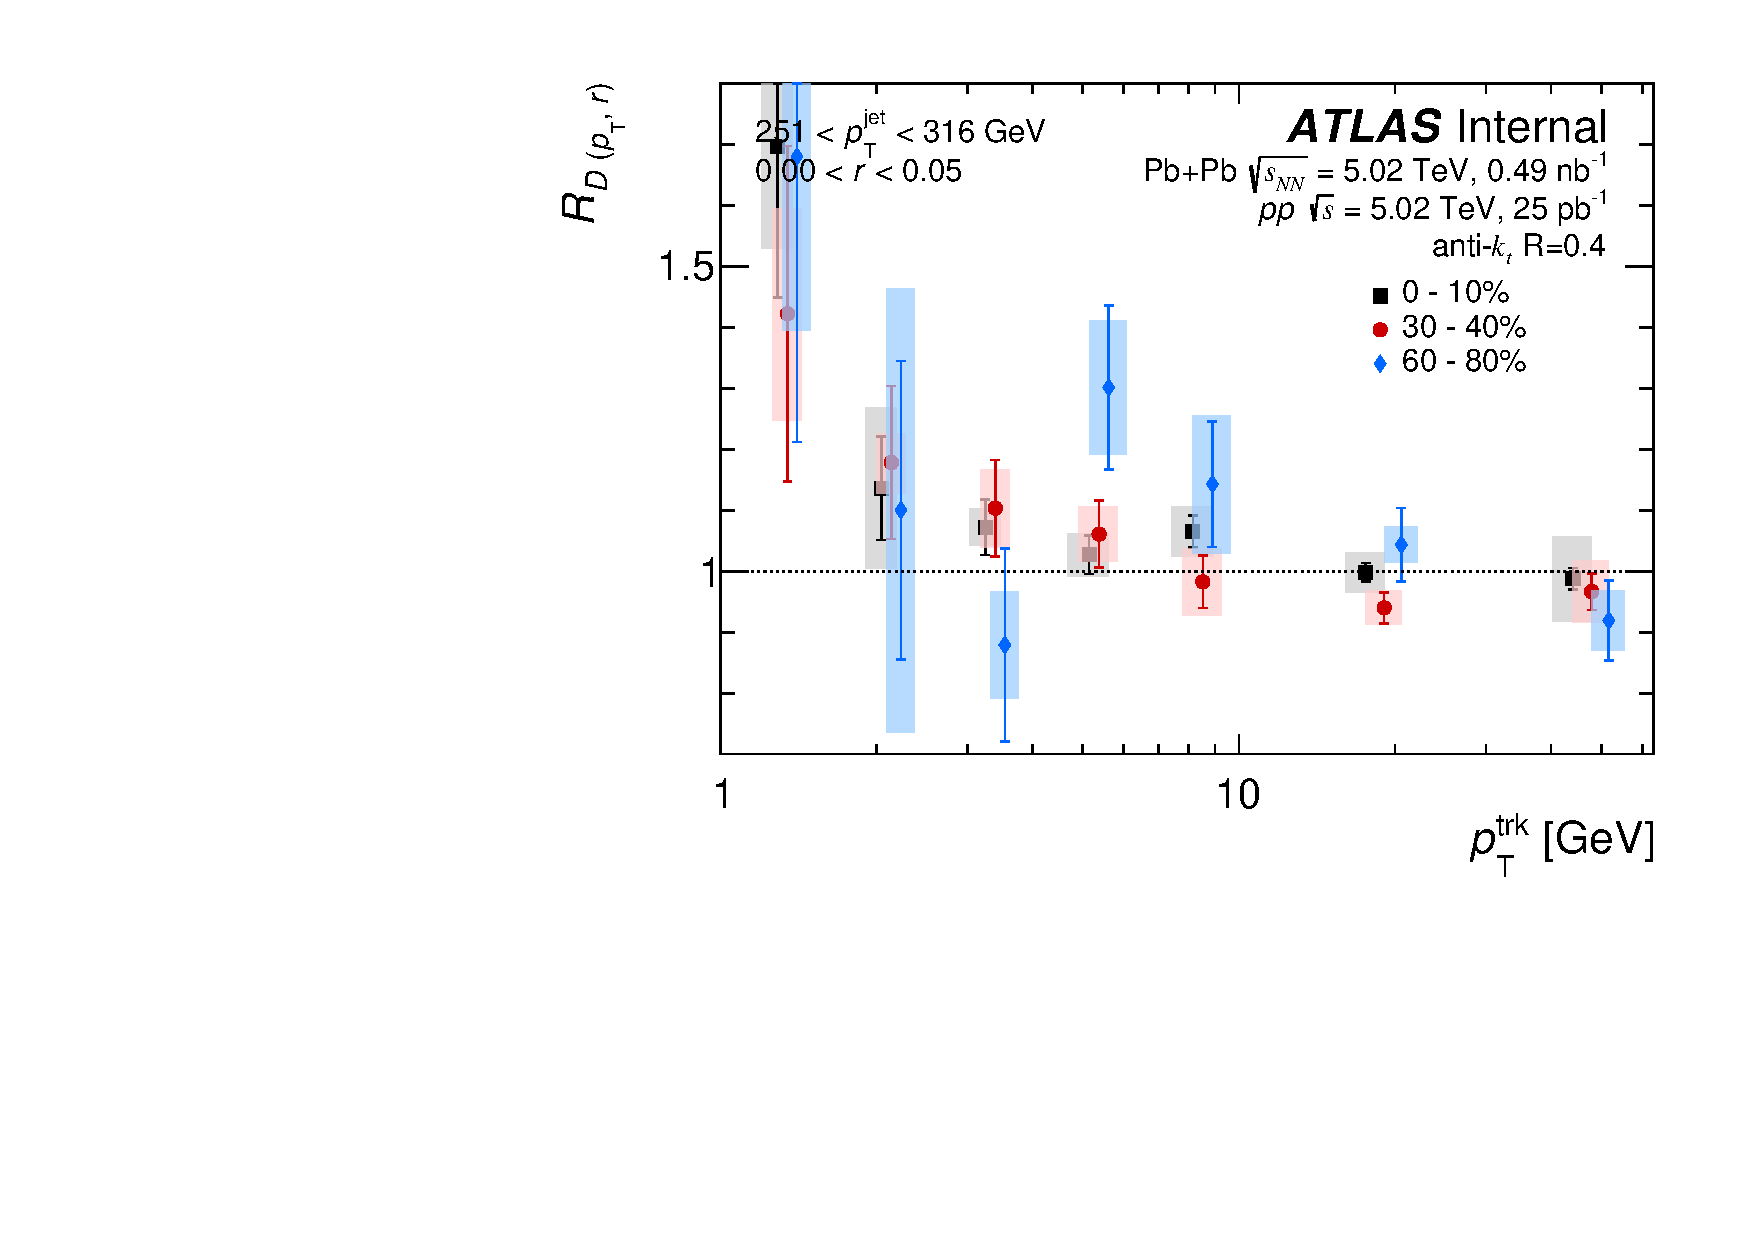
\includegraphics[width=0.5\textwidth]{figures/main/results/RDpT_trkpt_jet10_dR0} \\
%	 \includegraphics[width=0.5\textwidth]{figures/main/results/RDpT_trkpt_jet7_dR3} &
%	 \includegraphics[width=0.5\textwidth]{figures/main/results/RDpT_trkpt_jet9_dR3} \\
%	 \includegraphics[width=0.5\textwidth]{figures/main/results/RDpT_trkpt_jet7_dR10} &
%	 \includegraphics[width=0.5\textwidth]{figures/main/results/RDpT_trkpt_jet9_dR10} \\
%\end{tabular} }
%   \caption{\RDptr\ for central \pbpb\ collisions as a function of \pt\ for different jet selections.
%The different colors represent different centrality bins.
%The vertical bars on the data points indicate statistical uncertainties while the shaded boxes indicate systematic uncertainties.
%The widths of the boxes are not indicative of the bin size and the points are shifted horizontally for better visibility.}
%      \label{fig:rdptr_trk_cent}
%\end{figure}
%%%%%%%%%%%%%
%%%%%%%%%%%%%%%%%


\FloatBarrier


\subsection{Differences of \Dptr\ distributions}
In addition to the ratios of the \Dptr\ distributions, differences between the charged particle yields are also evaluated to quantify the modification in terms of the particle density.
These are given as:

\begin{align}
\DeltaDptr = \Dptr_{\mathrm{Pb+Pb}} - \Dptr_{pp}
\end{align}

These differences are presented as a function of $r$ for different \pt\ selections in 0--10\% central collisions in Figure~\ref{fig:deltadptr}.

These distributions show an excess  in the charged-particle yield density for \pbpb\ collisions compared to \pp\ collisions for charged particles with $\pt <4.0$ GeV.
This excess ranges from 0.5 to 4 particles per unit area at 1 \GeV\ in 126--158~\GeV\ jets for 0--10\% central \pbpb\ collisions and increases with increasing \ptjet.

The largest excesses for charged particles with $\pt <$~4.0~\GeV\ is within the jet cone.
 For large \rvar\ values, the
density decreases, but remains positive.
A depletion for higher \pt\ particles of approximately 0.5 particles per unit area is seen for 126--158~\GeV\ jets in 0--10\% central \pbpb\ collisions.
The magnitude of this depletion increases for higher \ptjet.

There is a minimum in the \DeltaDptr\ distributions of charged 
particles with \mbox{$ 4.0 < \pt <  25.1$}~\GeV\ at $0.05 < \rvar < 0.10$ that is seen at many \ptjet\ ranges under investigation.
The magnitudes of the excesses and deficits discussed here are dependent on the sizes of the charged-particle \pt\ selections
chosen.
 In order to remove that dependence, Section~\ref{sec:discussion_int} provides similar quantities in which a
wider charged-particle \pt\ range is integrated over.
%%%%%%%%%%%%%%%%%
%For particles with 25.1~$< \pt <$~63.1~\GeV, the \DeltaDptr\ distribution is consistent with unity over the entire measured range of \rvar\ and \ptjet.
%%%%%%%%%%%%%%%%%

\begin{figure}
\centering{
\begin{tabular}{cc}
	 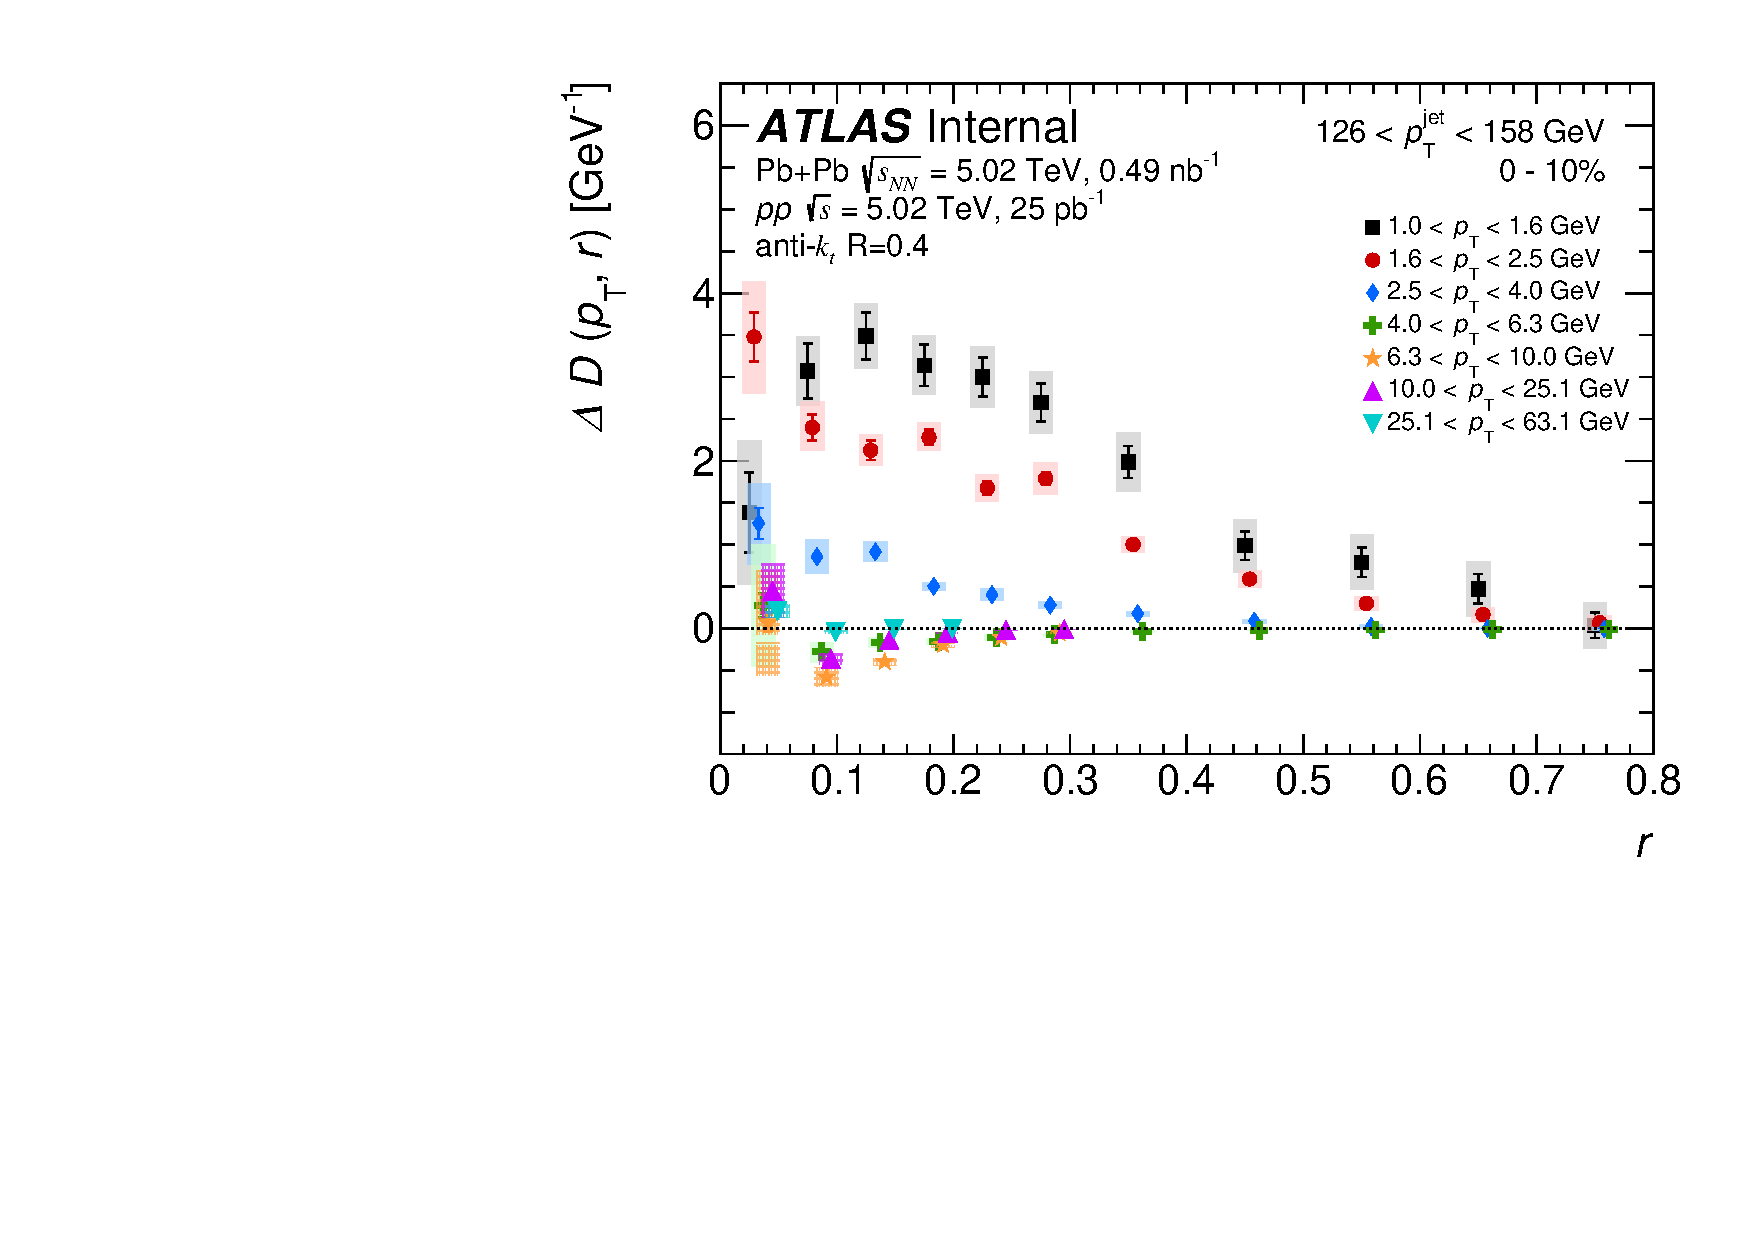
\includegraphics[width=0.5\textwidth]{figures/main/results/DeltaDpT_dR_jet7_cent0} &
	 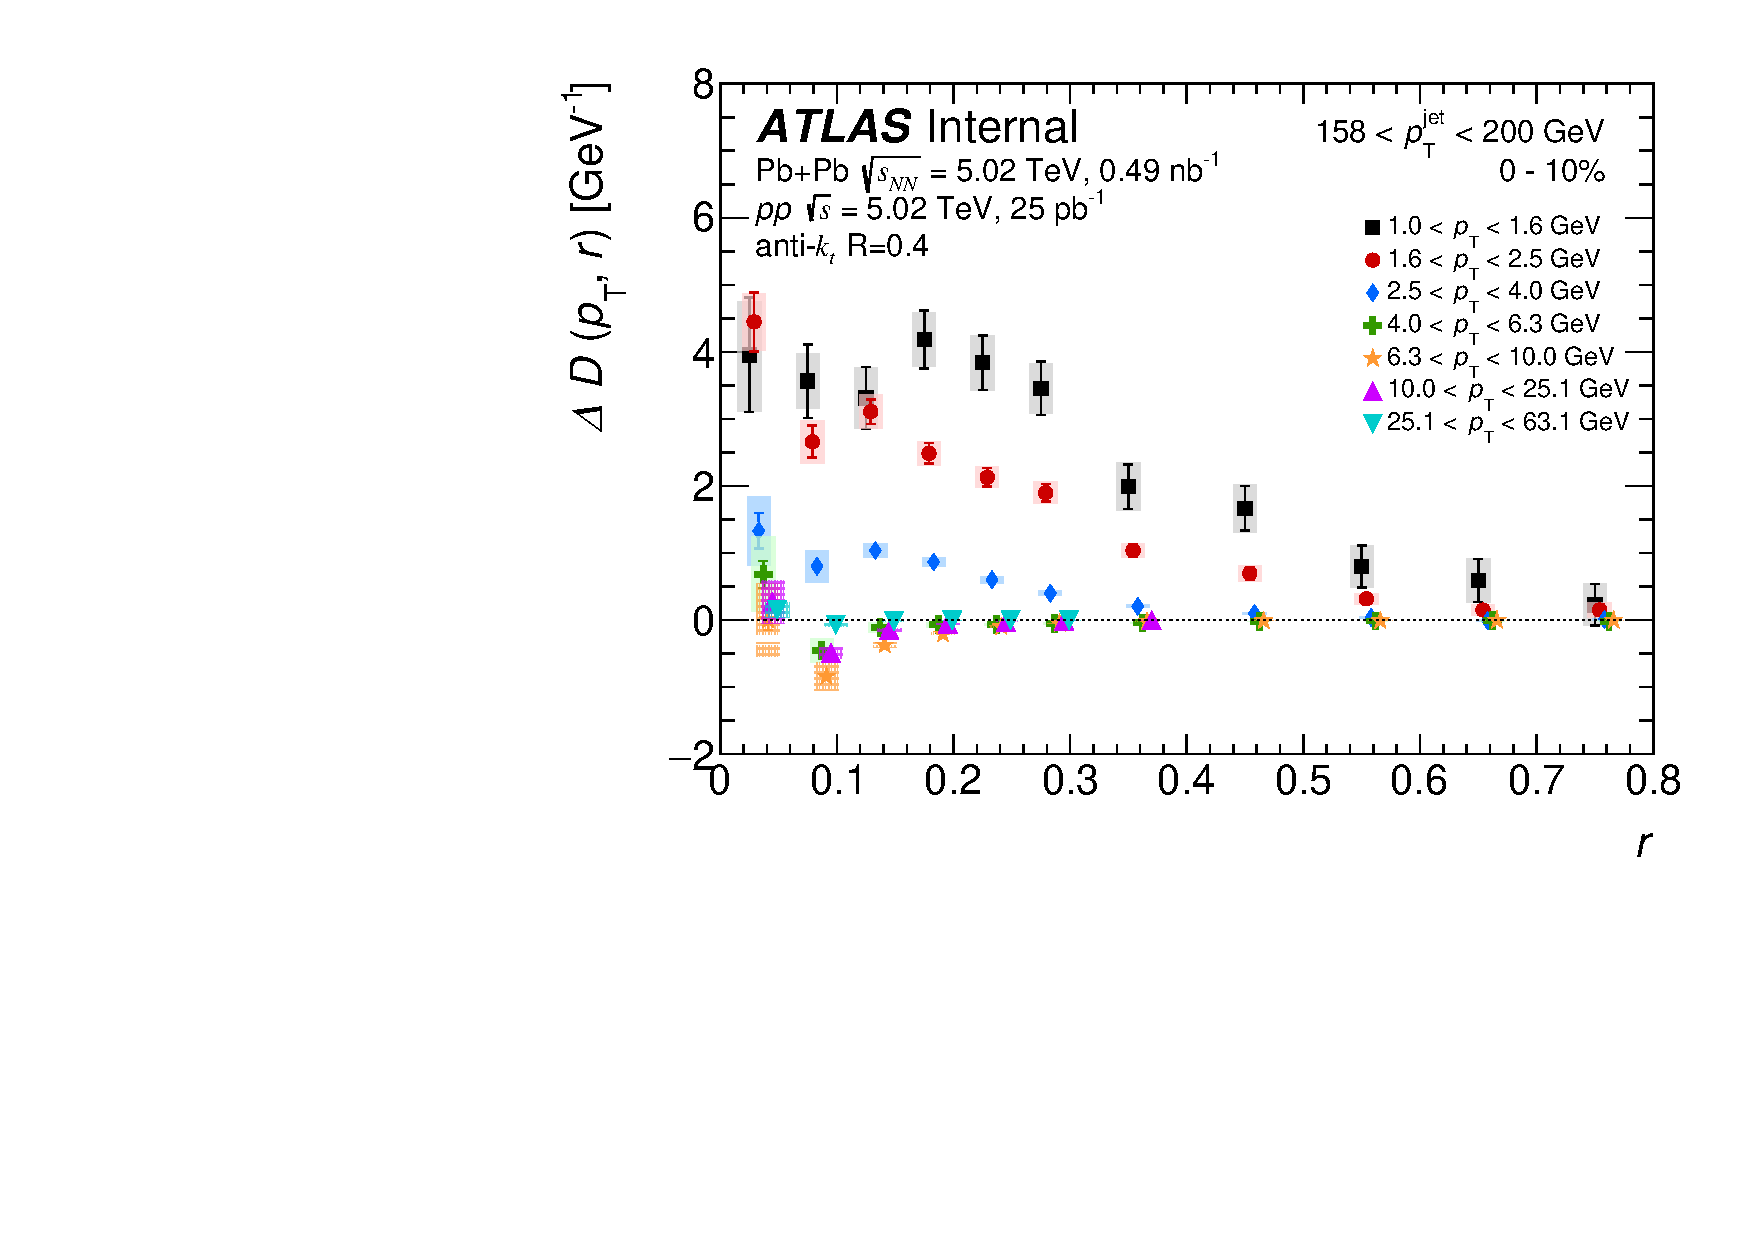
\includegraphics[width=0.5\textwidth]{figures/main/results/DeltaDpT_dR_jet8_cent0} \\
	 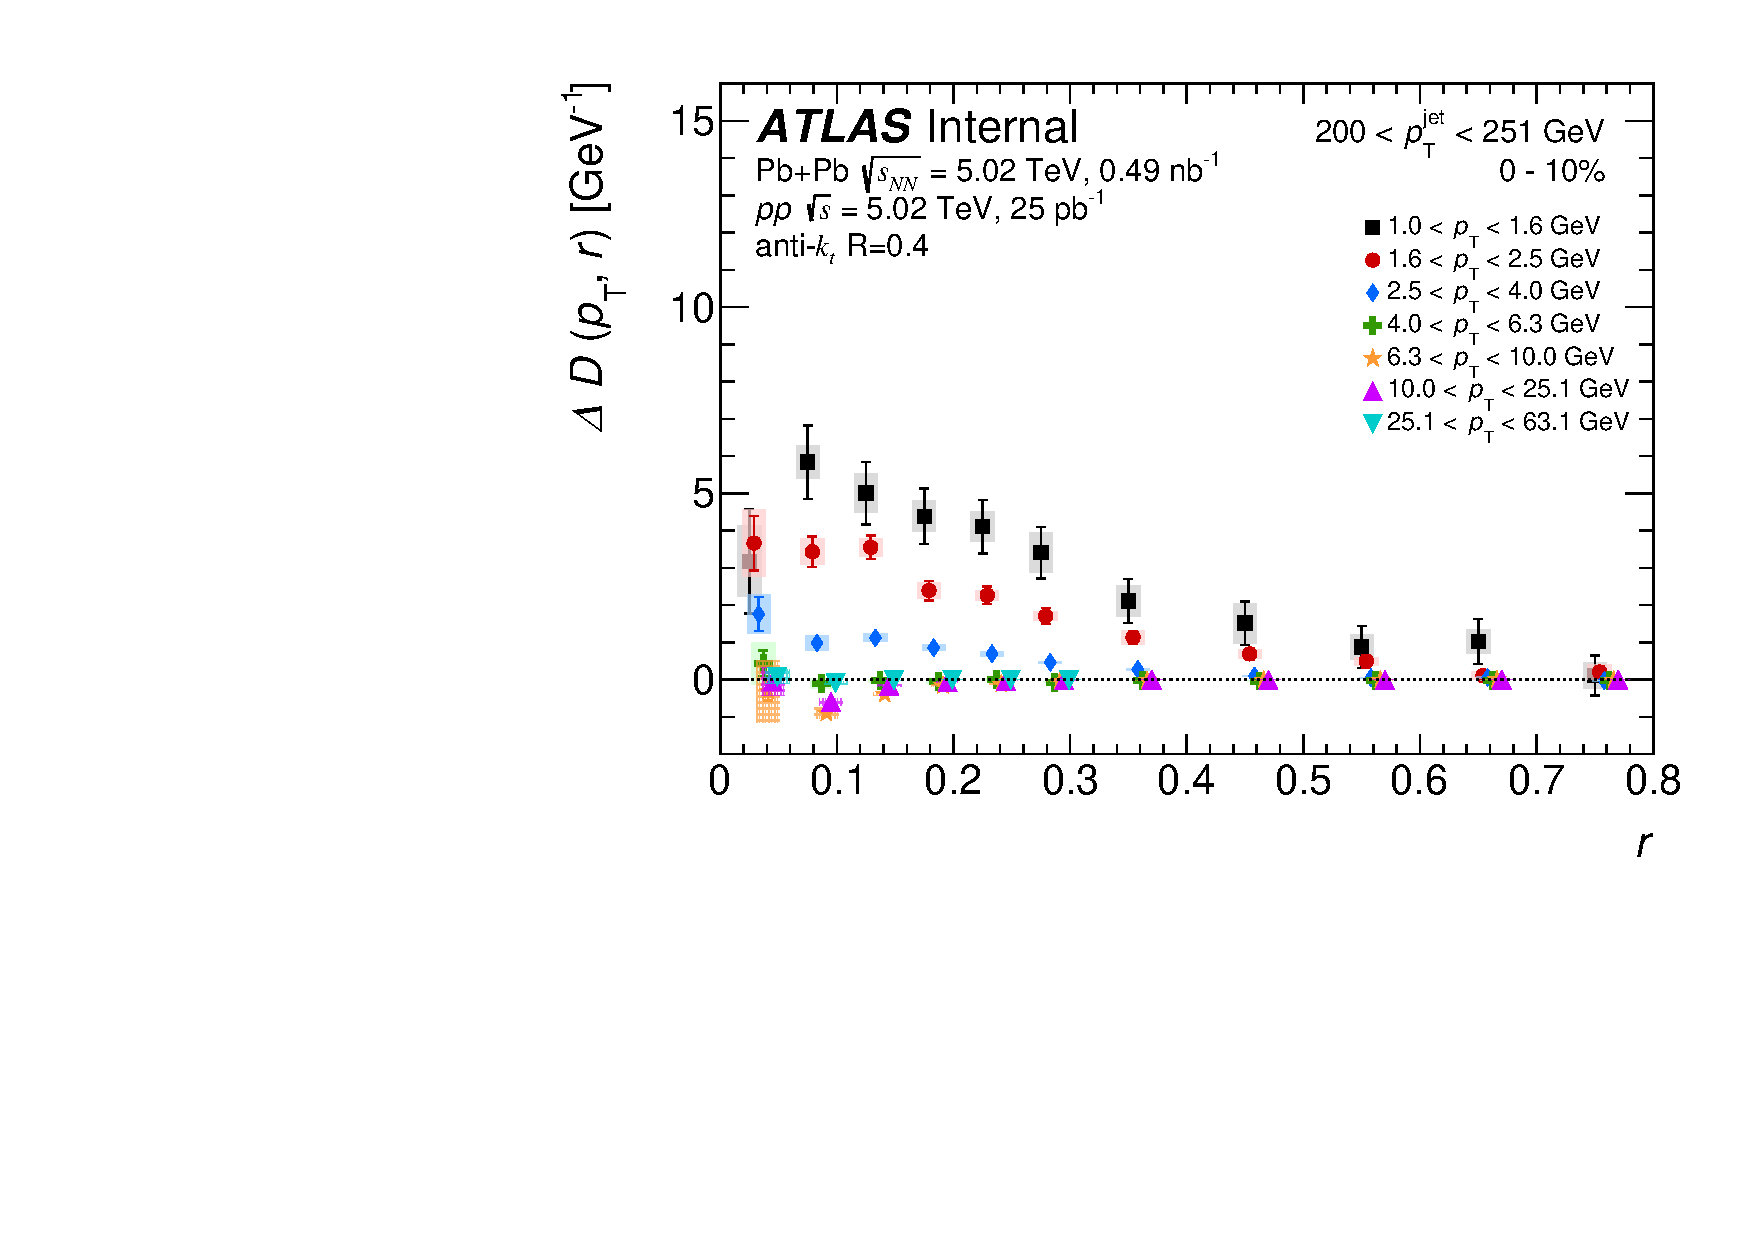
\includegraphics[width=0.5\textwidth]{figures/main/results/DeltaDpT_dR_jet9_cent0} &
	 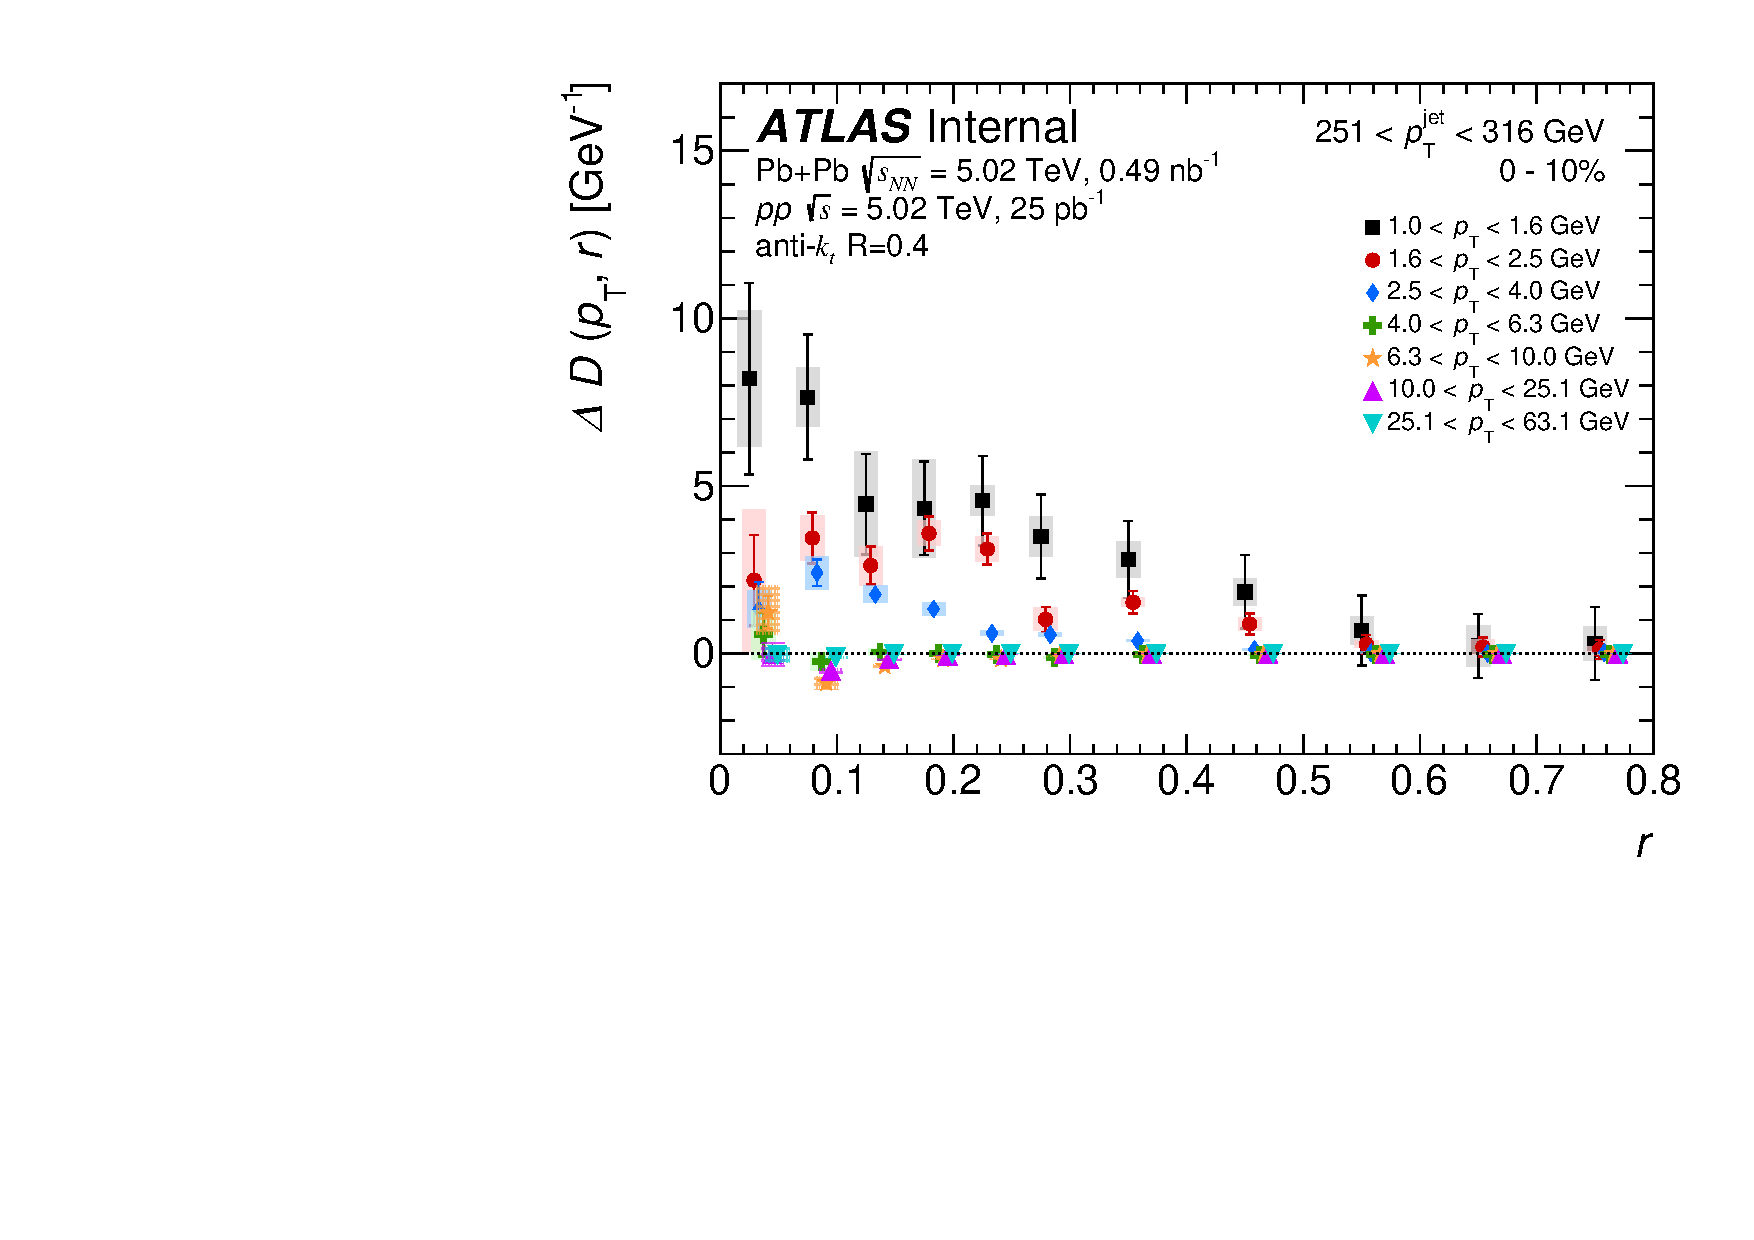
\includegraphics[width=0.5\textwidth]{figures/main/results/DeltaDpT_dR_jet10_cent0} \\
\end{tabular} }
   \caption{\DeltaDptr\ as a function of \rvar\ in central collisions for all \pt\ ranges in four \ptjet\ selections: 126--158~\GeV, 158--200~\GeV, 200--251~\GeV, and 251--316~\GeV.
The vertical bars on the data points indicate statistical uncertainties while the shaded boxes indicate systematic uncertainties.
The widths of the boxes are not indicative of the bin size and the points are shifted horizontally for better visibility.
}
      \label{fig:deltadptr}
\end{figure}
%%%%%%%%%%%%%
\FloatBarrier

\subsection{\pt\ integrated distributions}
\label{sec:discussion_int}
Motivated by similar studies of the enhancement of soft fragments in 
jet fragmentation functions in \pbpb\ compared to \pp\ collisions from \cite{PhysRevC.98.024908}, the \Dptr\ distributions can be integrated for charged particles with \pt\ < 4 GeV to construct the quantities $\Theta(\rvar)$ and $P(\rvar)$ defined as:

\begin{align}
   \Theta(\rvar) &= \int_1^{4} \Dptr  \fd \pt \\
   P(\rvar) &= \int_0^r \int_1^{4} \Dptr \fd \pt \fd r'
\end{align}

The $\Theta(\rvar)$ values are integrated between 1.0--4.0~\GeV\ charged particles to provide a summary look at
the \pt\ region of enhancement discussed above.
 The $P(\rvar)$ values further add a running integral over \rvar\
and provide information about the jet shape.
Both of these quantities can be compared between the \pp\ and \pbpb\ systems to give the following distributions:

\begin{align}
   \Delta_{\Theta(\rvar)} &= \Theta(\rvar)_{\mathrm{Pb+Pb}} - \Theta(\rvar)_{pp} \\
   R_{\Theta(\rvar)} &= \frac{\Theta(\rvar)_{\mathrm{Pb+Pb}}}{\Theta(\rvar)_{\mathrm{pp}}} \\
   R_{P(\rvar)} &= \frac{P(\rvar)_{\mathrm{Pb+Pb}}}{P(\rvar)_{pp}}
\end{align}

(the quantity $\Delta_{P(\rvar)}$ can also be analogously defined, but is omitted from the present discussion).
These aggregate quantities are intended to provide some summary information about the location with respect to the 
jet axis, magnitude, and \ptjet\ dependence of the low-\pt\ charged-particle excess discussed above.
The ratio quantities are useful for comparisons to other \pbpb\ measurements; $\Delta_{\Theta(\rvar)}$ is very similar 
to $\DeltaDptr$, however it is integrated over charged-particle \pt\ from 1.0--4.0~\GeV.

Figure~\ref{fig:deltaPdeltaT} shows the \DeltaTheta\ distributions as a function of \rvar\ for 0--10\%, 30--40\%,
and 60--80\% central collisions.

In the most central collisions, a significant \ptjet\ dependence to \DeltaTheta\ is observed; for $\rvar <$~0.4 (particles
within the jet cone) \DeltaTheta\ increases with increasing \ptjet.
The value of \DeltaTheta\ decreases in more peripheral collisions and the \ptjet\ dependence is no longer significant.

%%%%%%%%%%%%%%%%%
%Now, the \ptjet\ dependence to the excess in charged-particle density can be seen clearly; 
%in the most central collisions
%there is an increase in \DeltaTheta\ with increasing \ptjet, but in the mid-central and peripheral collisions this is no longer
%observed within the uncertainties.
%%%%%%%%%%%%%%%%%

\begin{figure}
\centering{
\begin{tabular}{ccc}
	 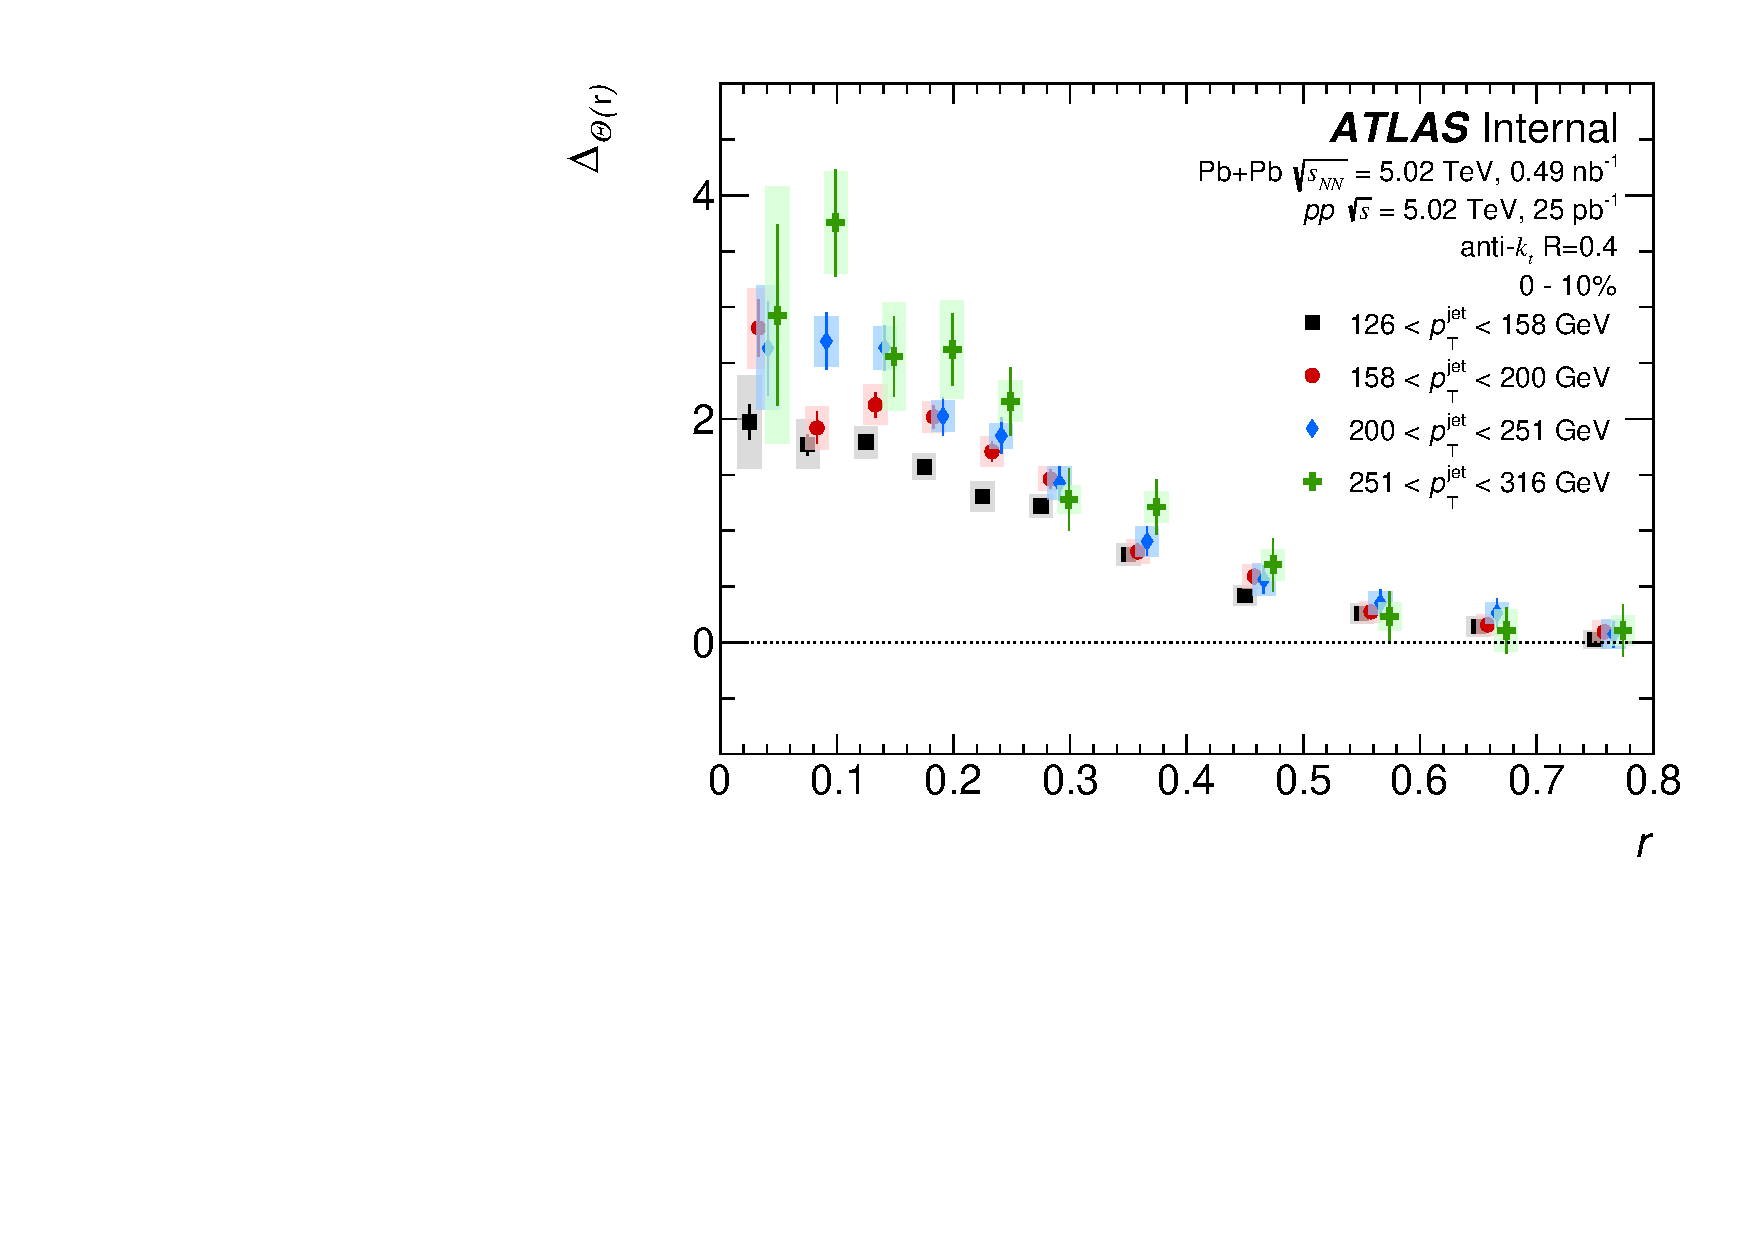
\includegraphics[width=0.3\textwidth]{figures/main/results/DeltaDpT_lowpt_integ_cent0.pdf} &
   %	 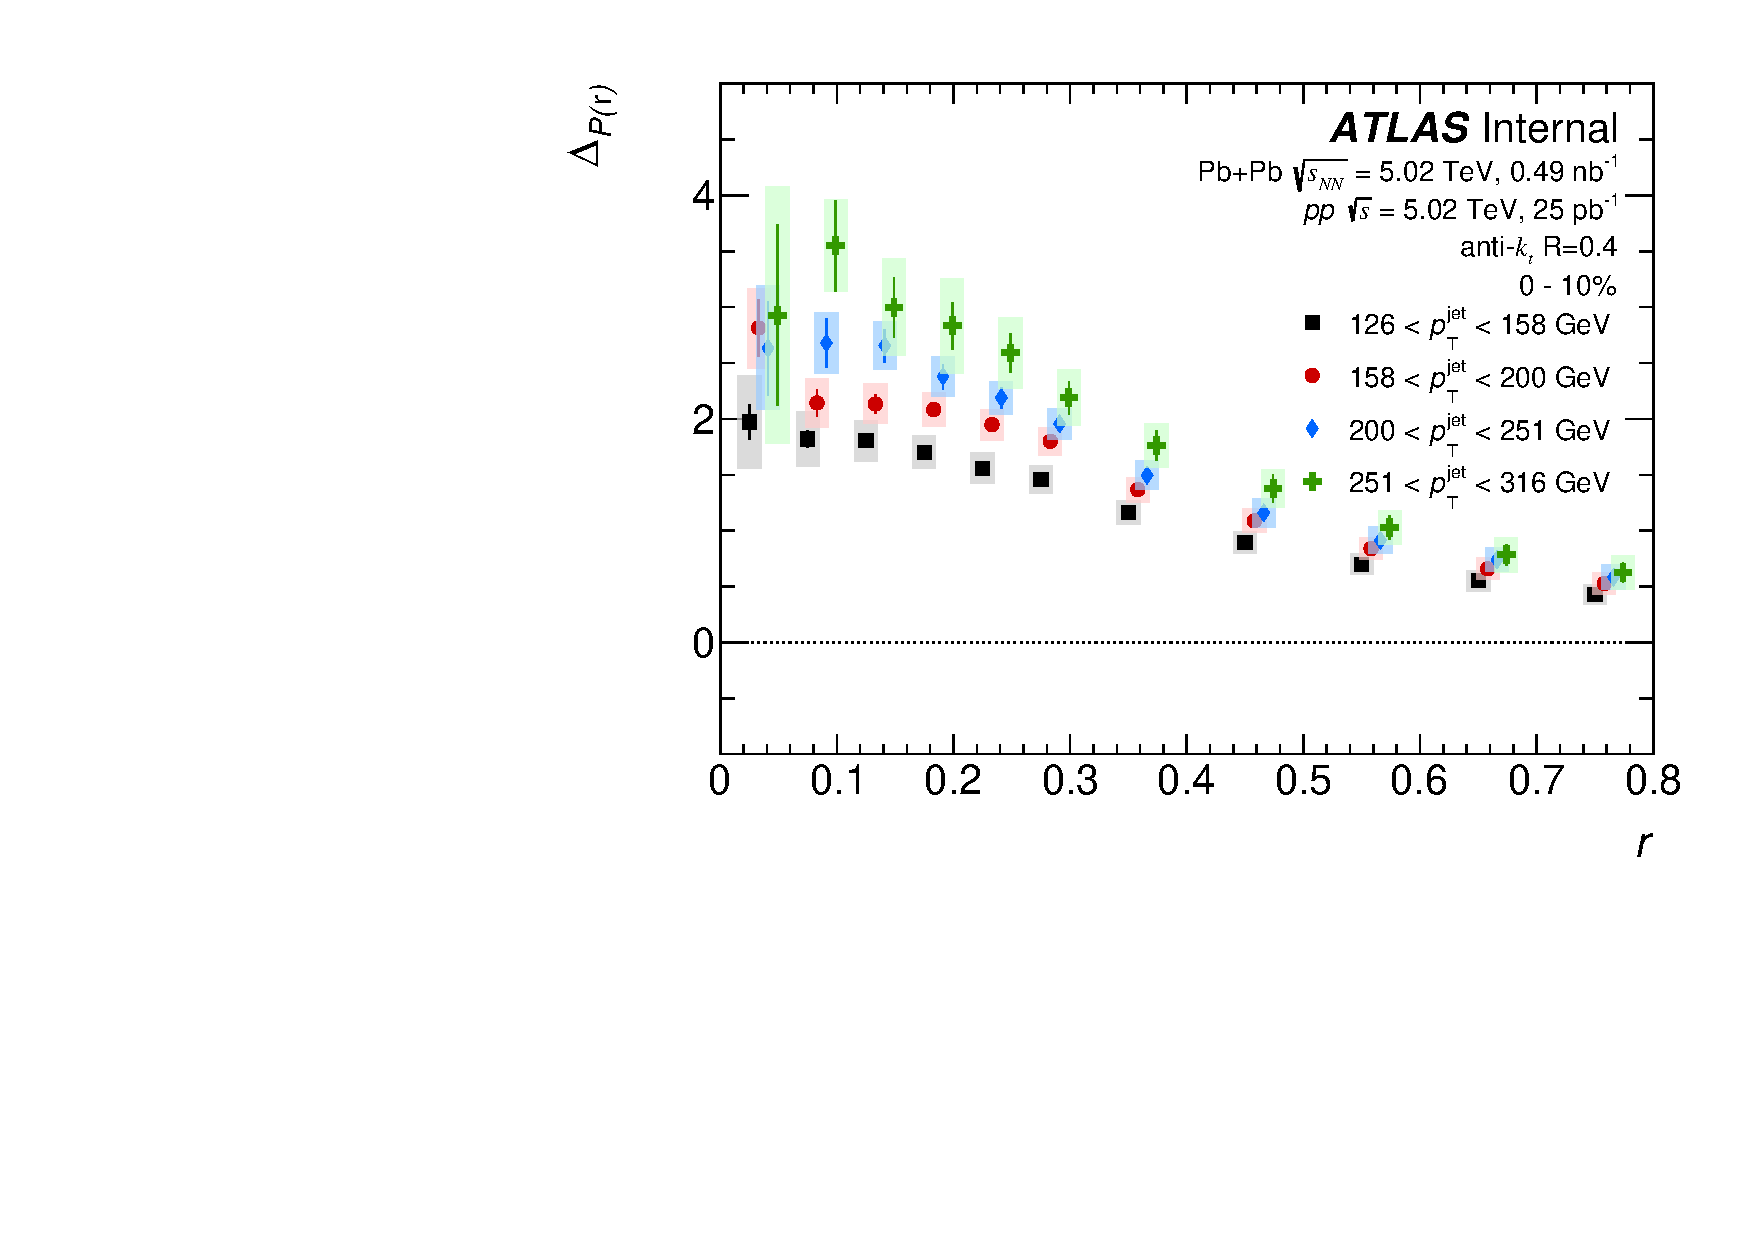
\includegraphics[width=0.5\textwidth]{figures/main/results/DeltaDpT_jetshape_cent0.pdf} \\
	 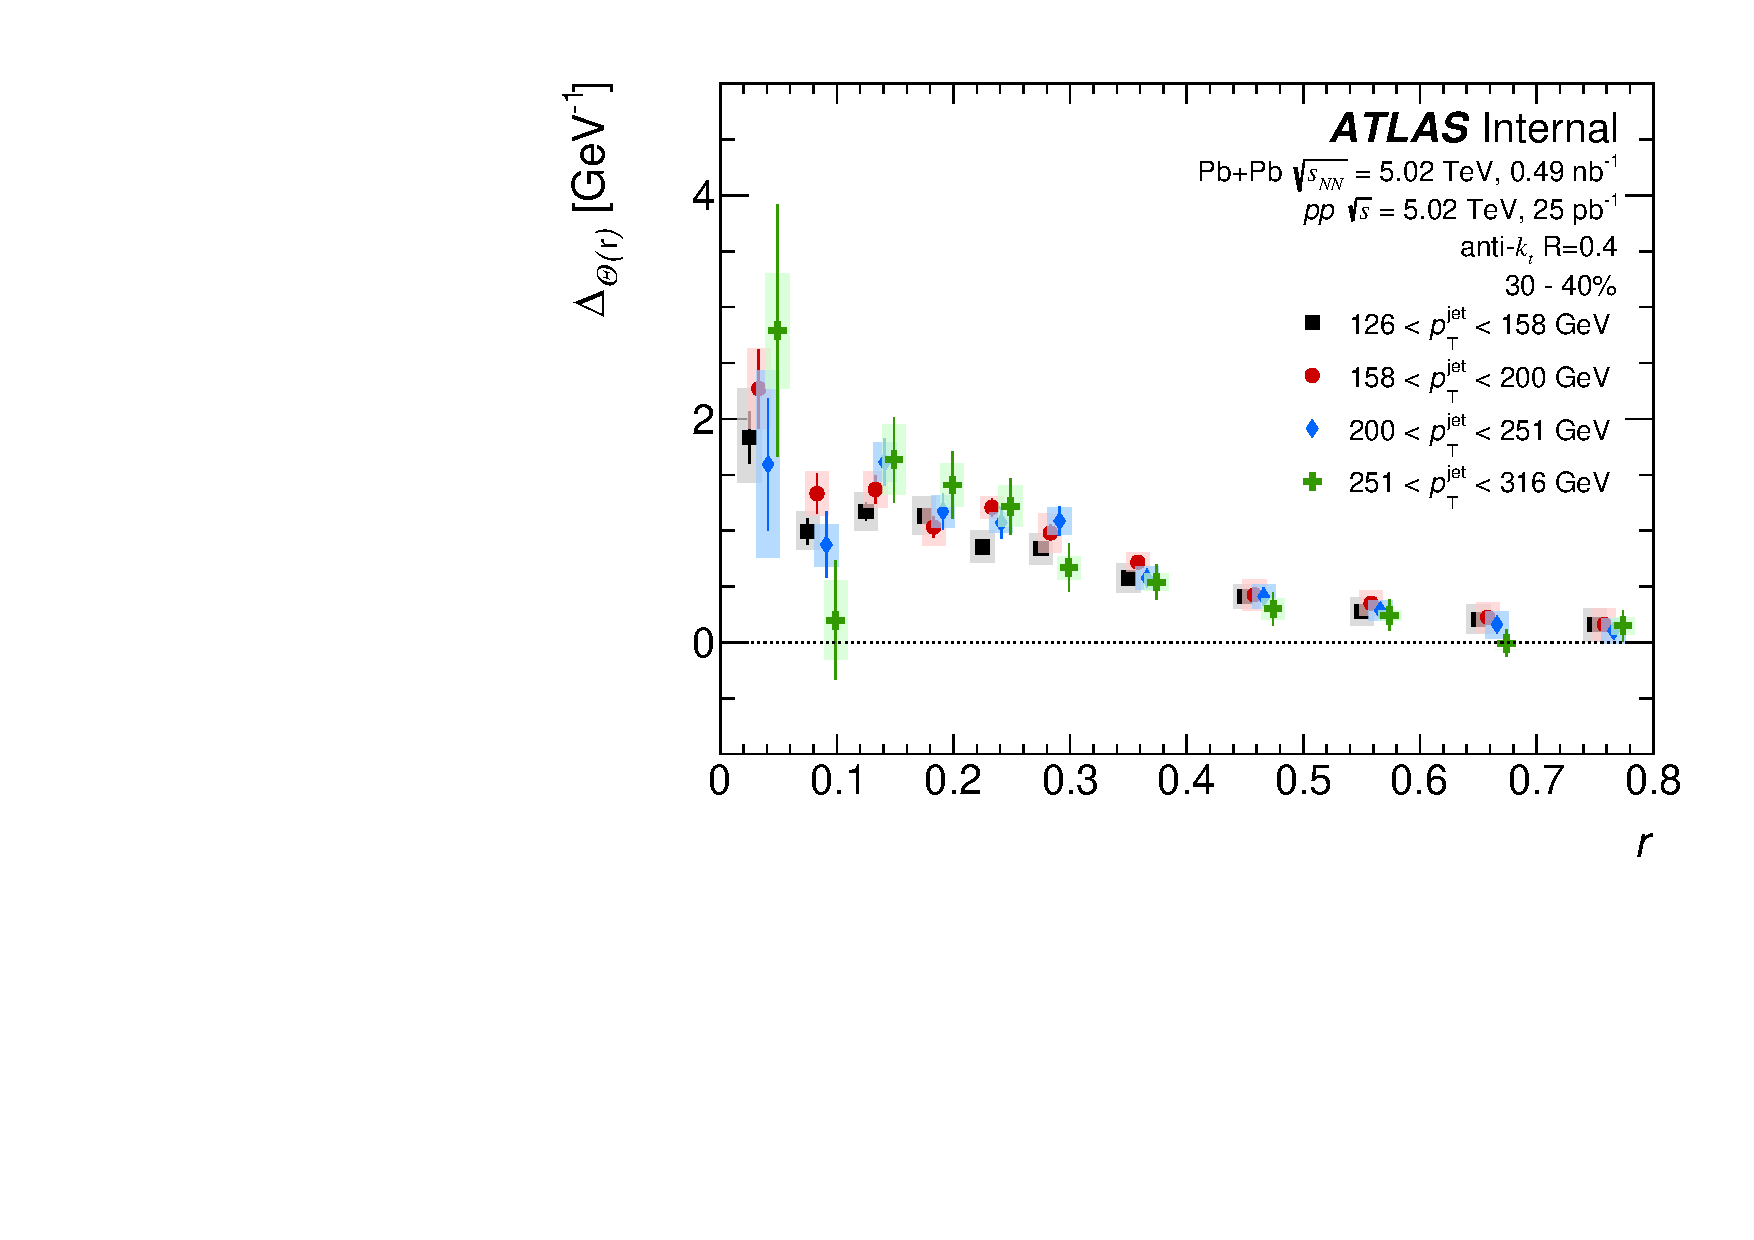
\includegraphics[width=0.3\textwidth]{figures/main/results/DeltaDpT_lowpt_integ_cent3.pdf} &
%	 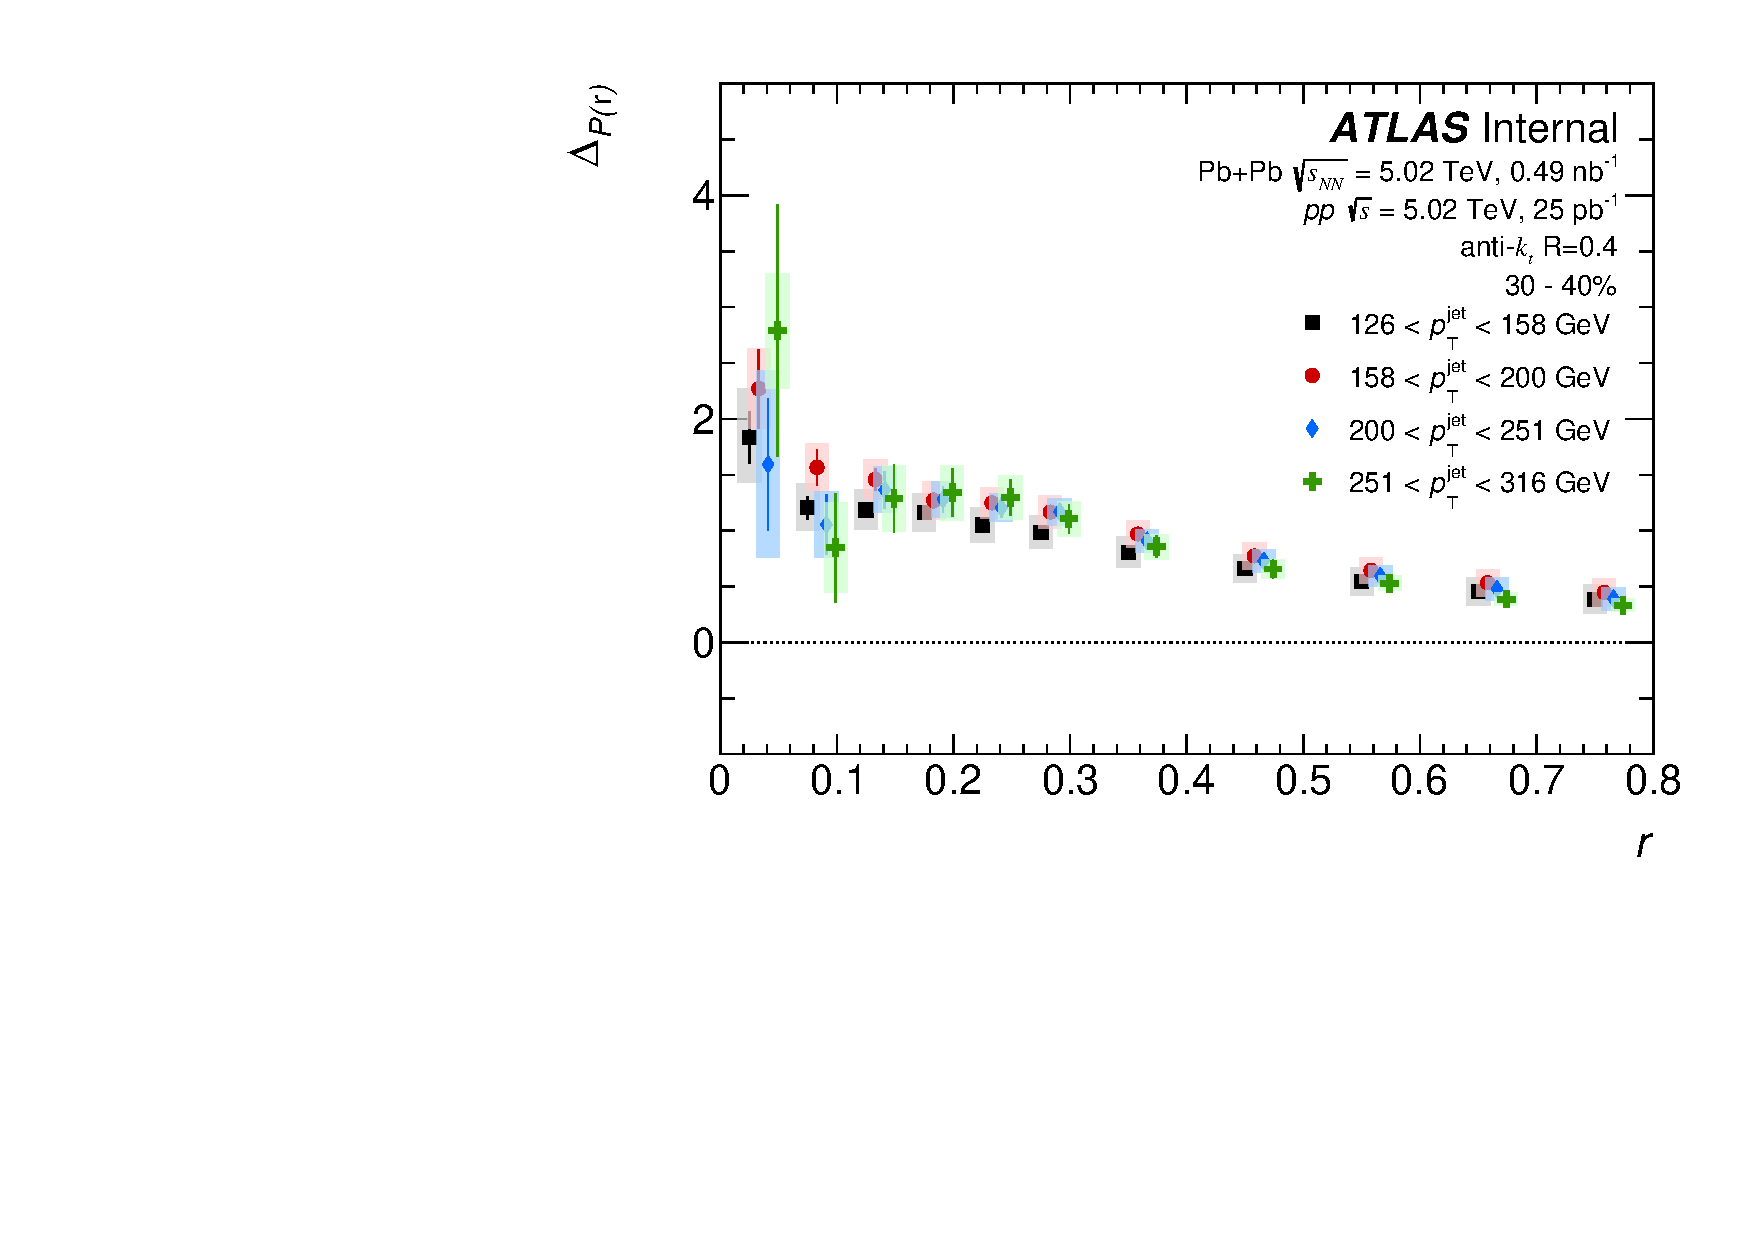
\includegraphics[width=0.5\textwidth]{figures/main/results/DeltaDpT_jetshape_cent3.pdf} \\
	 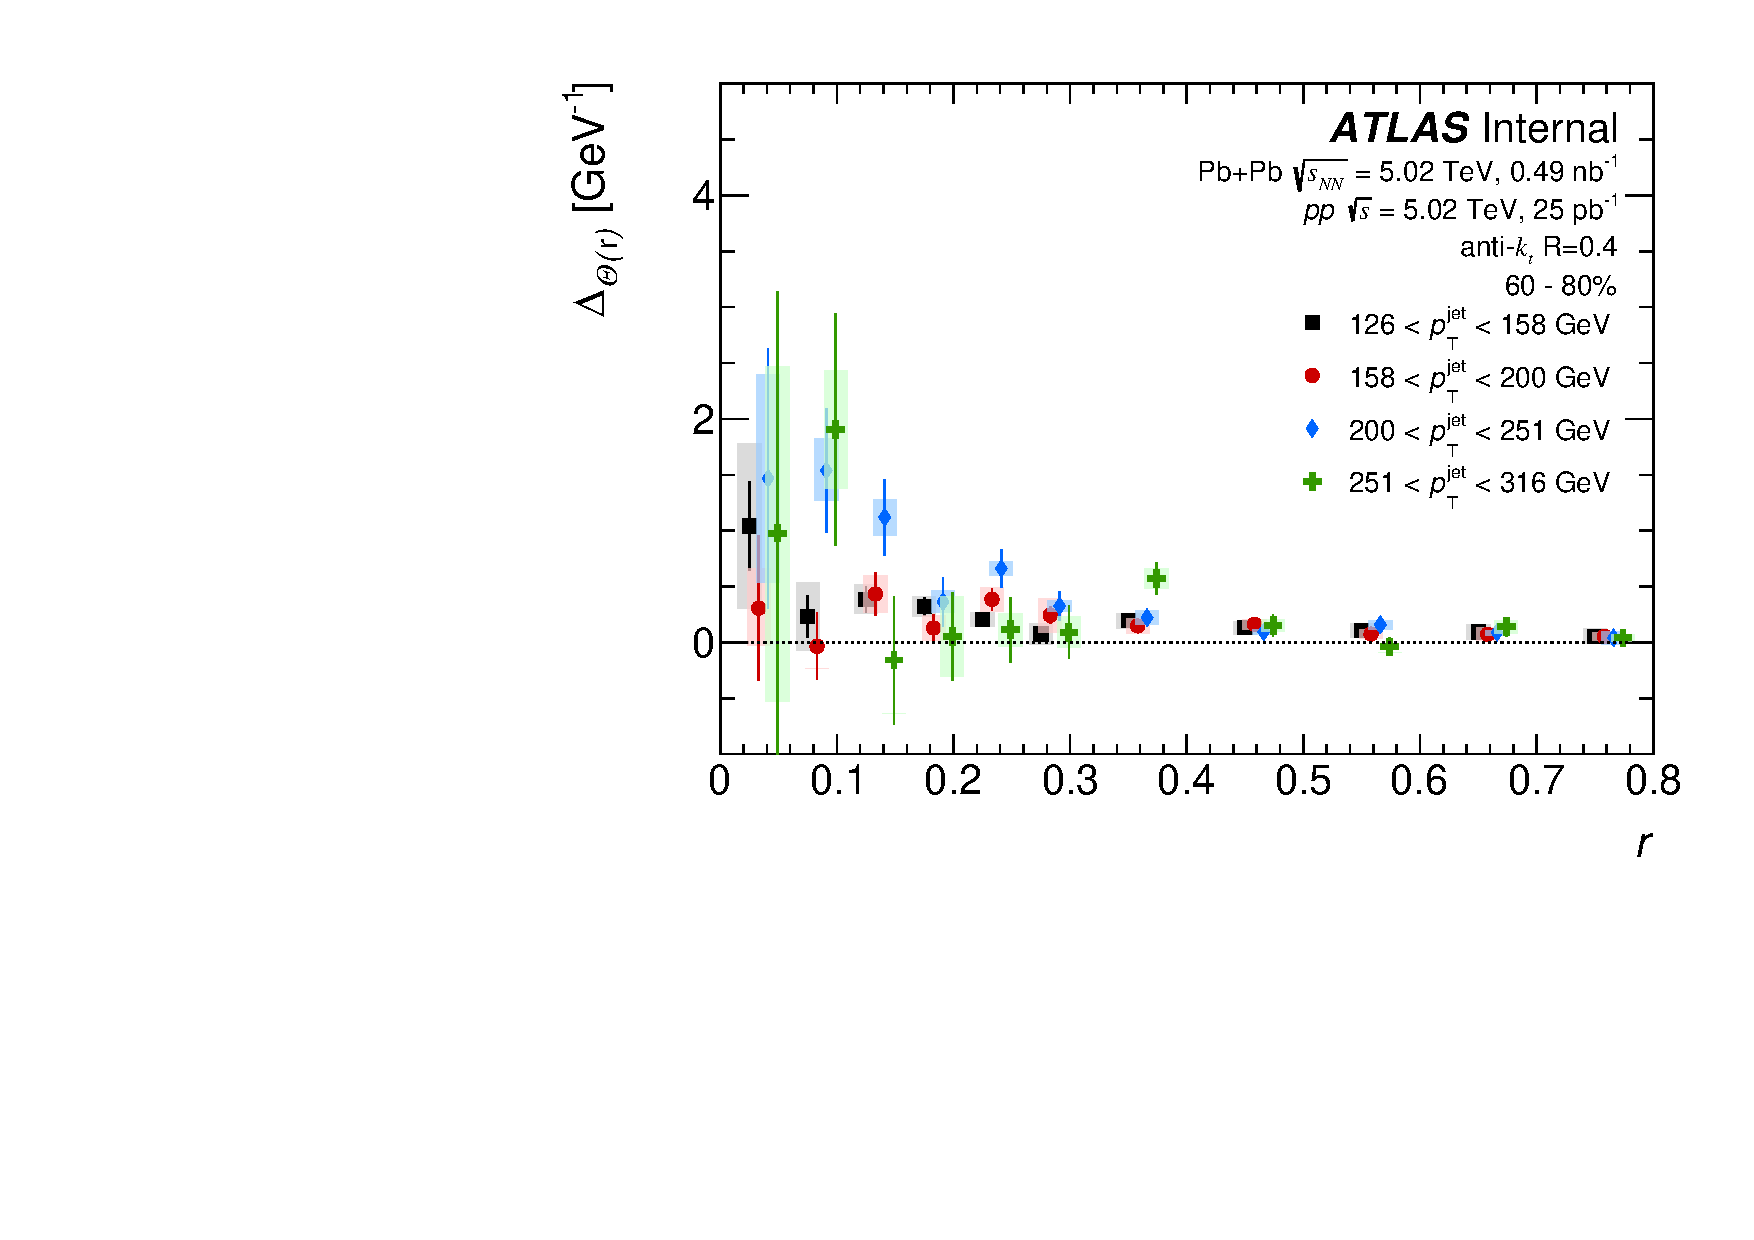
\includegraphics[width=0.3\textwidth]{figures/main/results/DeltaDpT_lowpt_integ_cent5.pdf} \\
%	 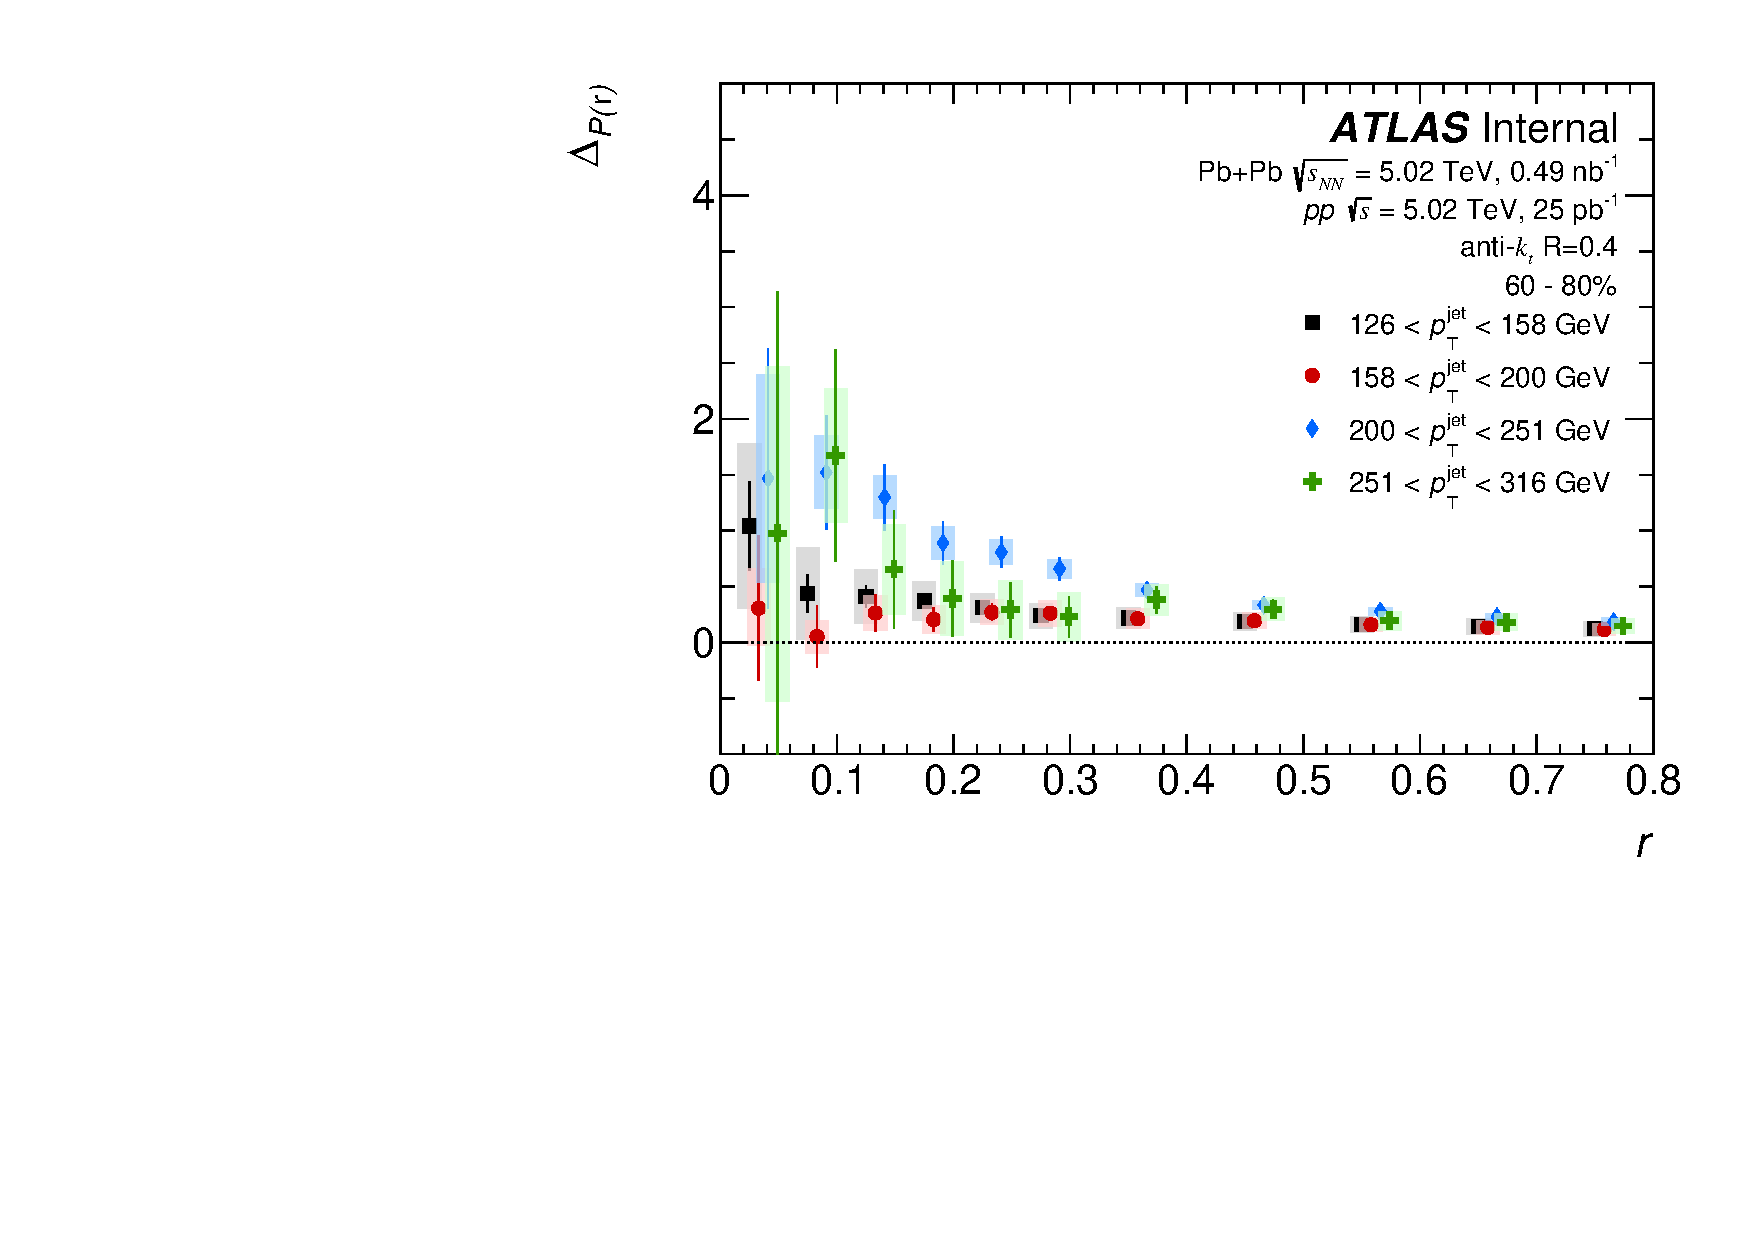
\includegraphics[width=0.5\textwidth]{figures/main/results/DeltaDpT_jetshape_cent5.pdf} \\
\end{tabular} }
   \caption{\DeltaTheta\ as a function of \rvar\ for charged-particles with \pt\ < 4 GeV ranges in 
   four \ptjet\ selections: 126--158~\GeV, 158--200~\GeV, 200--251~\GeV, and 251--316~\GeV and three centrality 
   selections: 0--10\% (left), 30--40\% (middle) and 60--80\% (right).
   The vertical bars on the data points indicate statistical uncertainties while the shaded boxes indicate systematic uncertainties.
The widths of the boxes are not indicative of the bin size and the points are shifted horizontally for better visibility.
}
      \label{fig:deltaPdeltaT}
\end{figure}


\begin{figure}
\centering{
\begin{tabular}{cc}
	 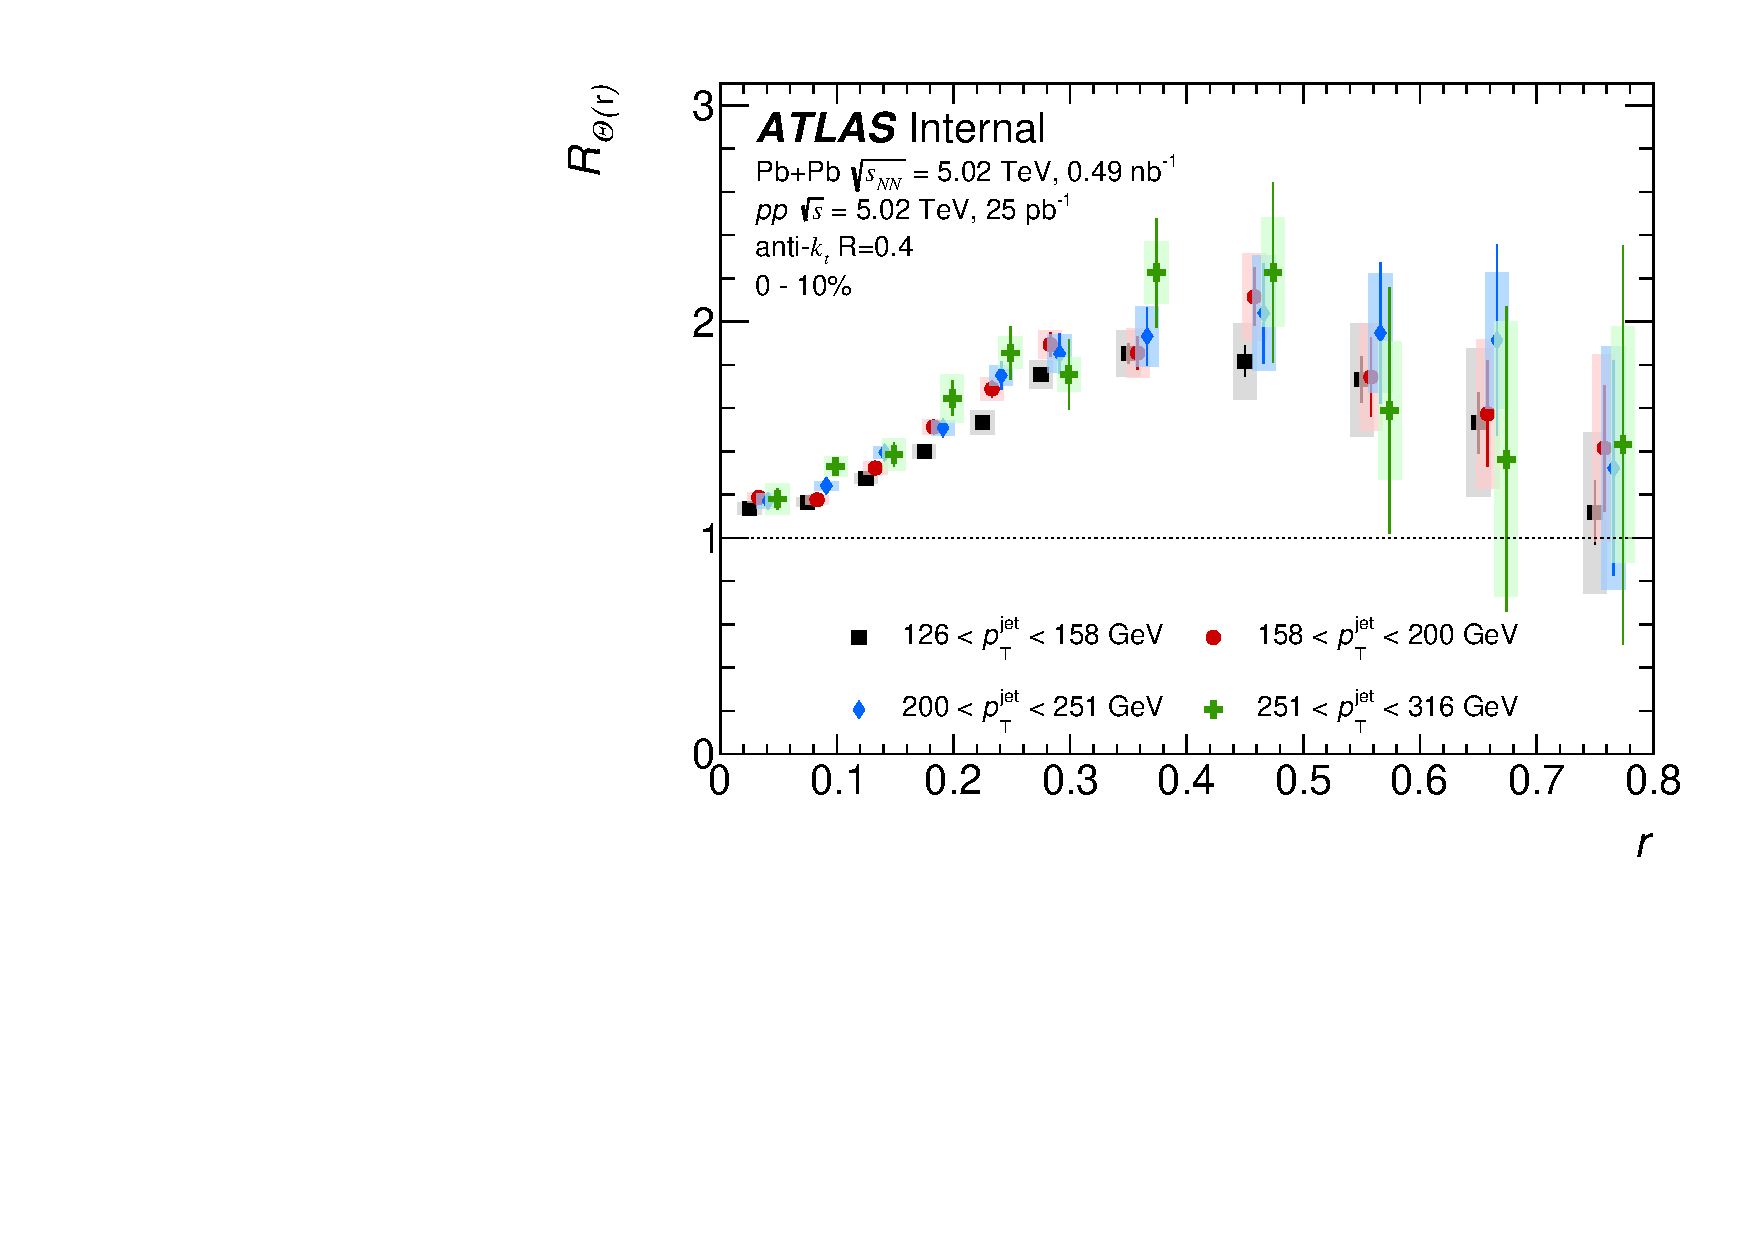
\includegraphics[width=0.5\textwidth]{figures/main/results/RDpT_lowpt_integ_cent0.pdf} &
	 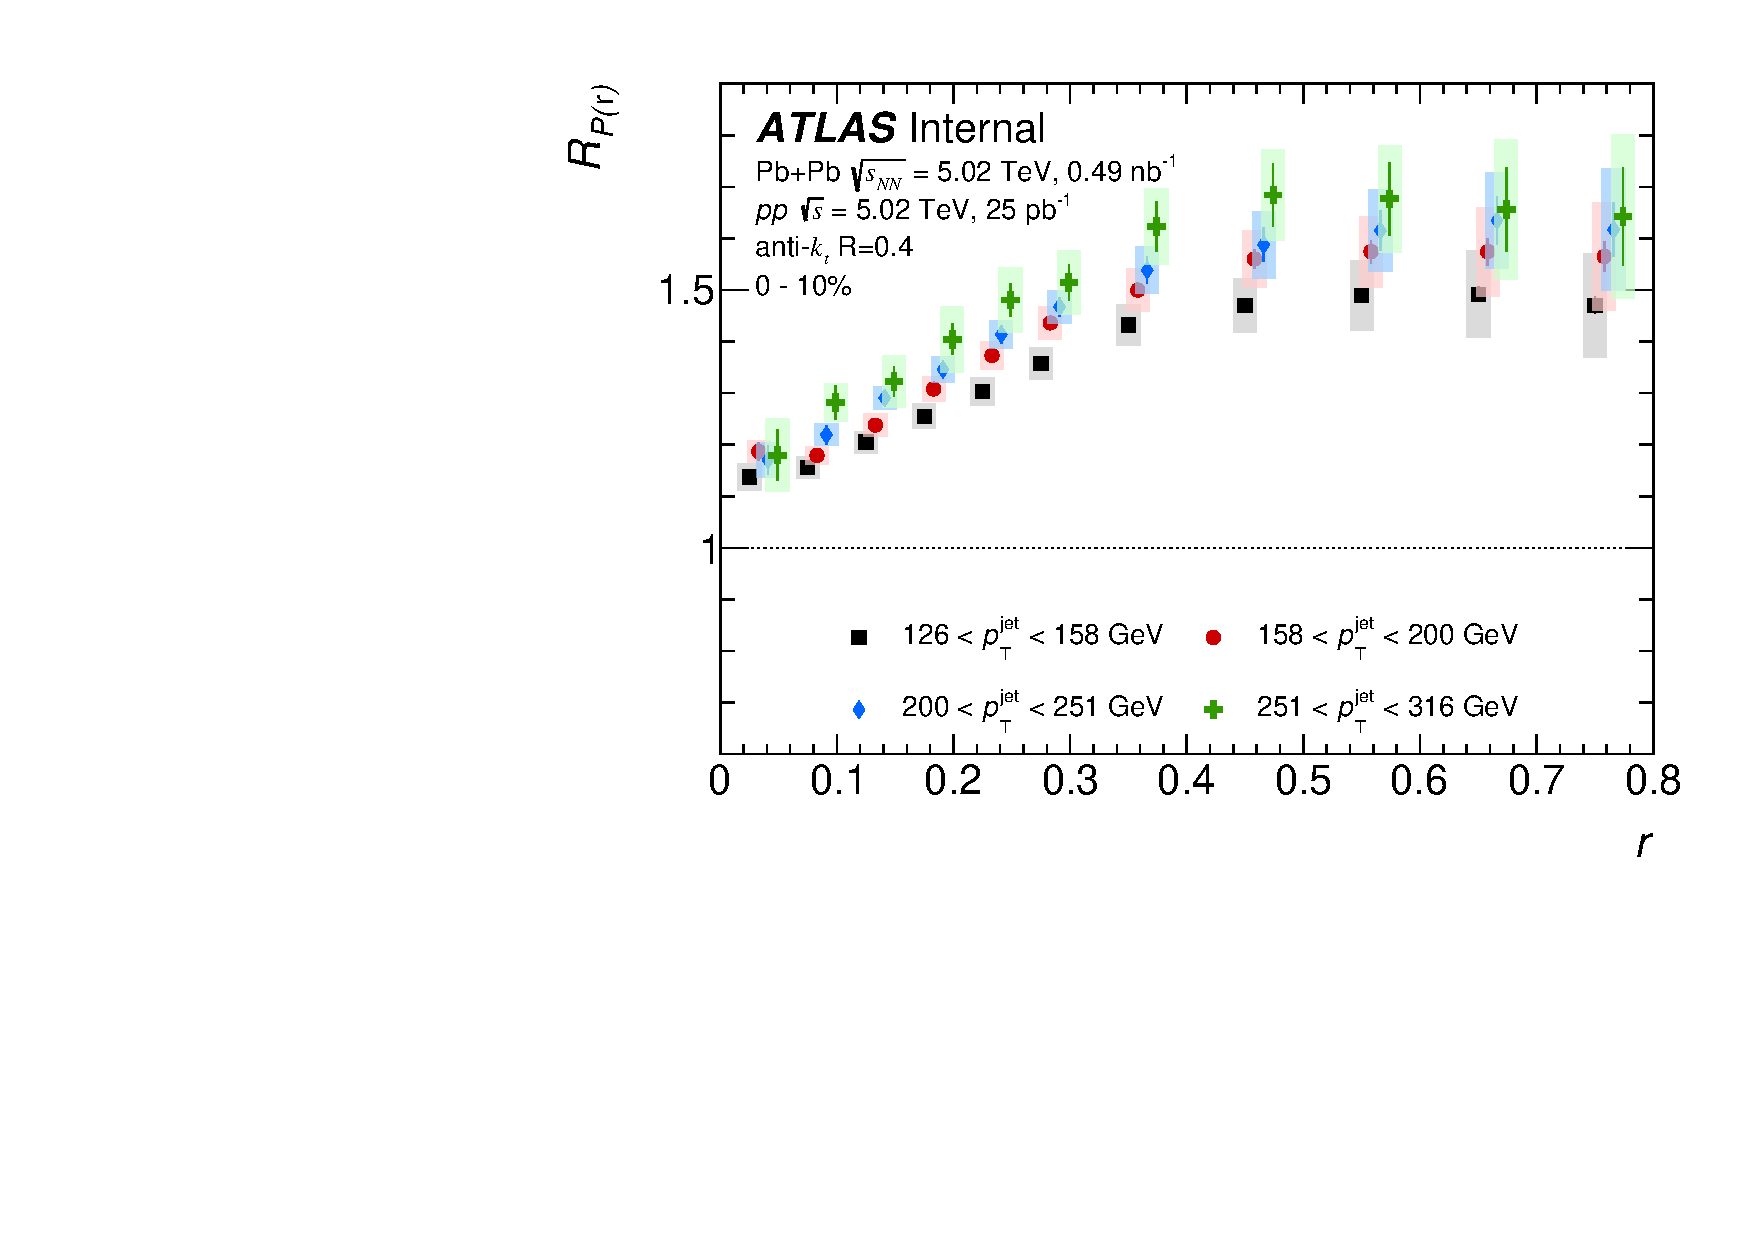
\includegraphics[width=0.5\textwidth]{figures/main/results/RDpT_jetshape_cent0.pdf} \\
	 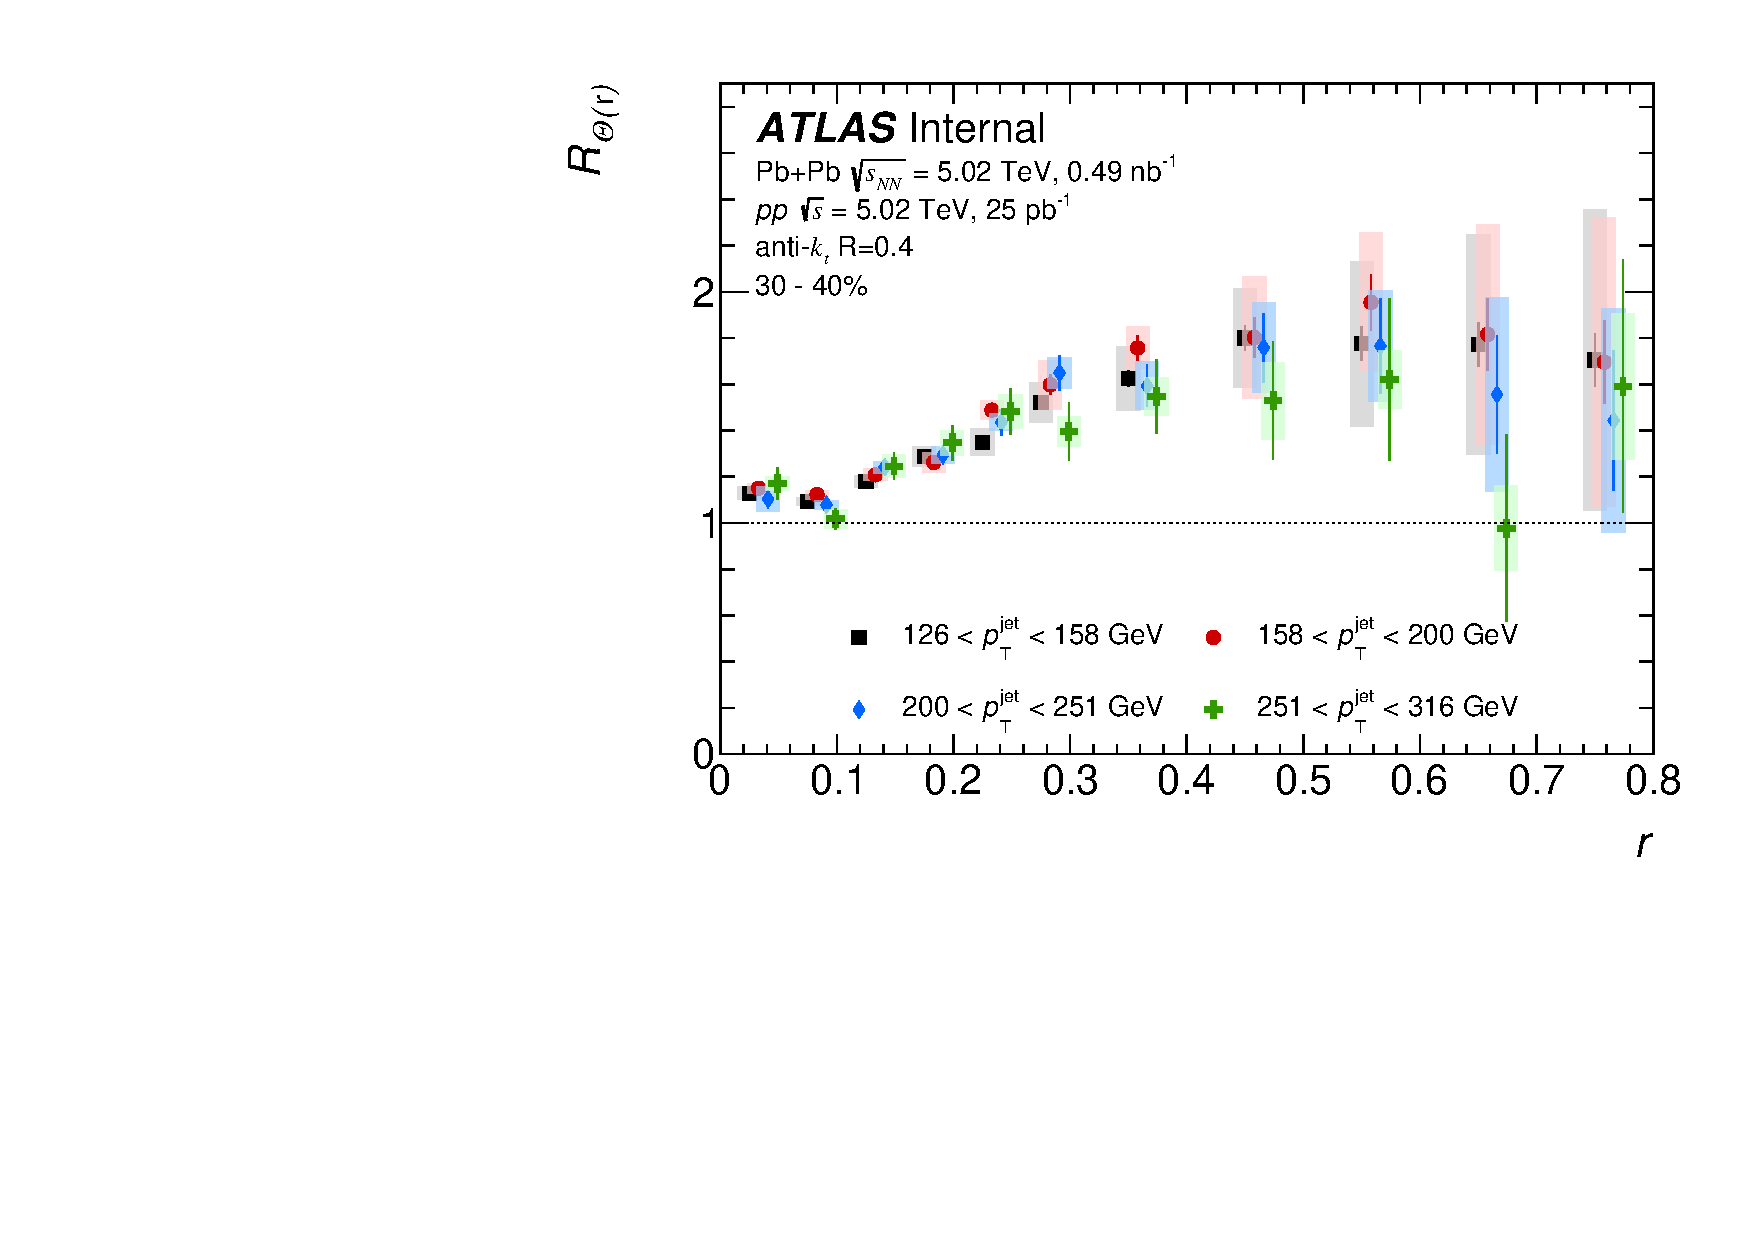
\includegraphics[width=0.5\textwidth]{figures/main/results/RDpT_lowpt_integ_cent3.pdf} &
	 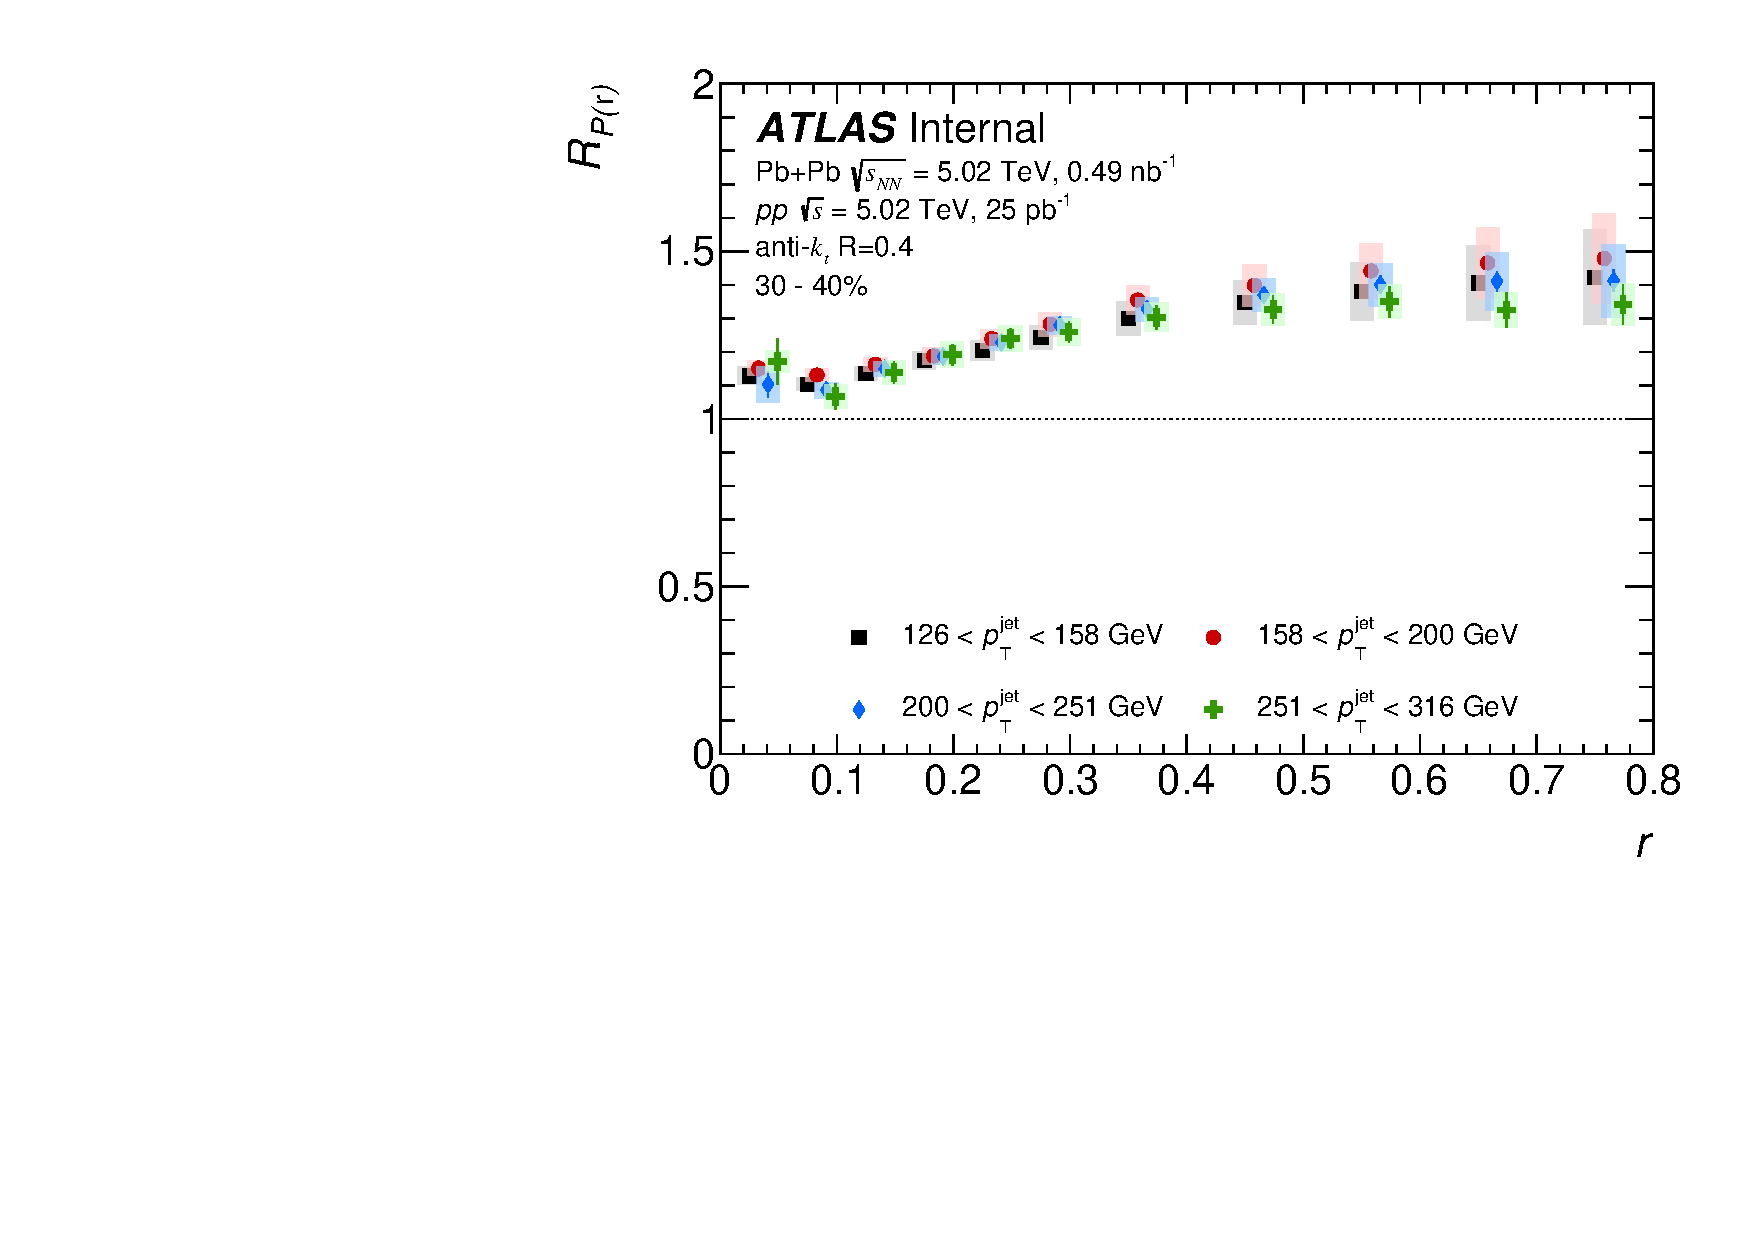
\includegraphics[width=0.5\textwidth]{figures/main/results/RDpT_jetshape_cent3.pdf} \\
	 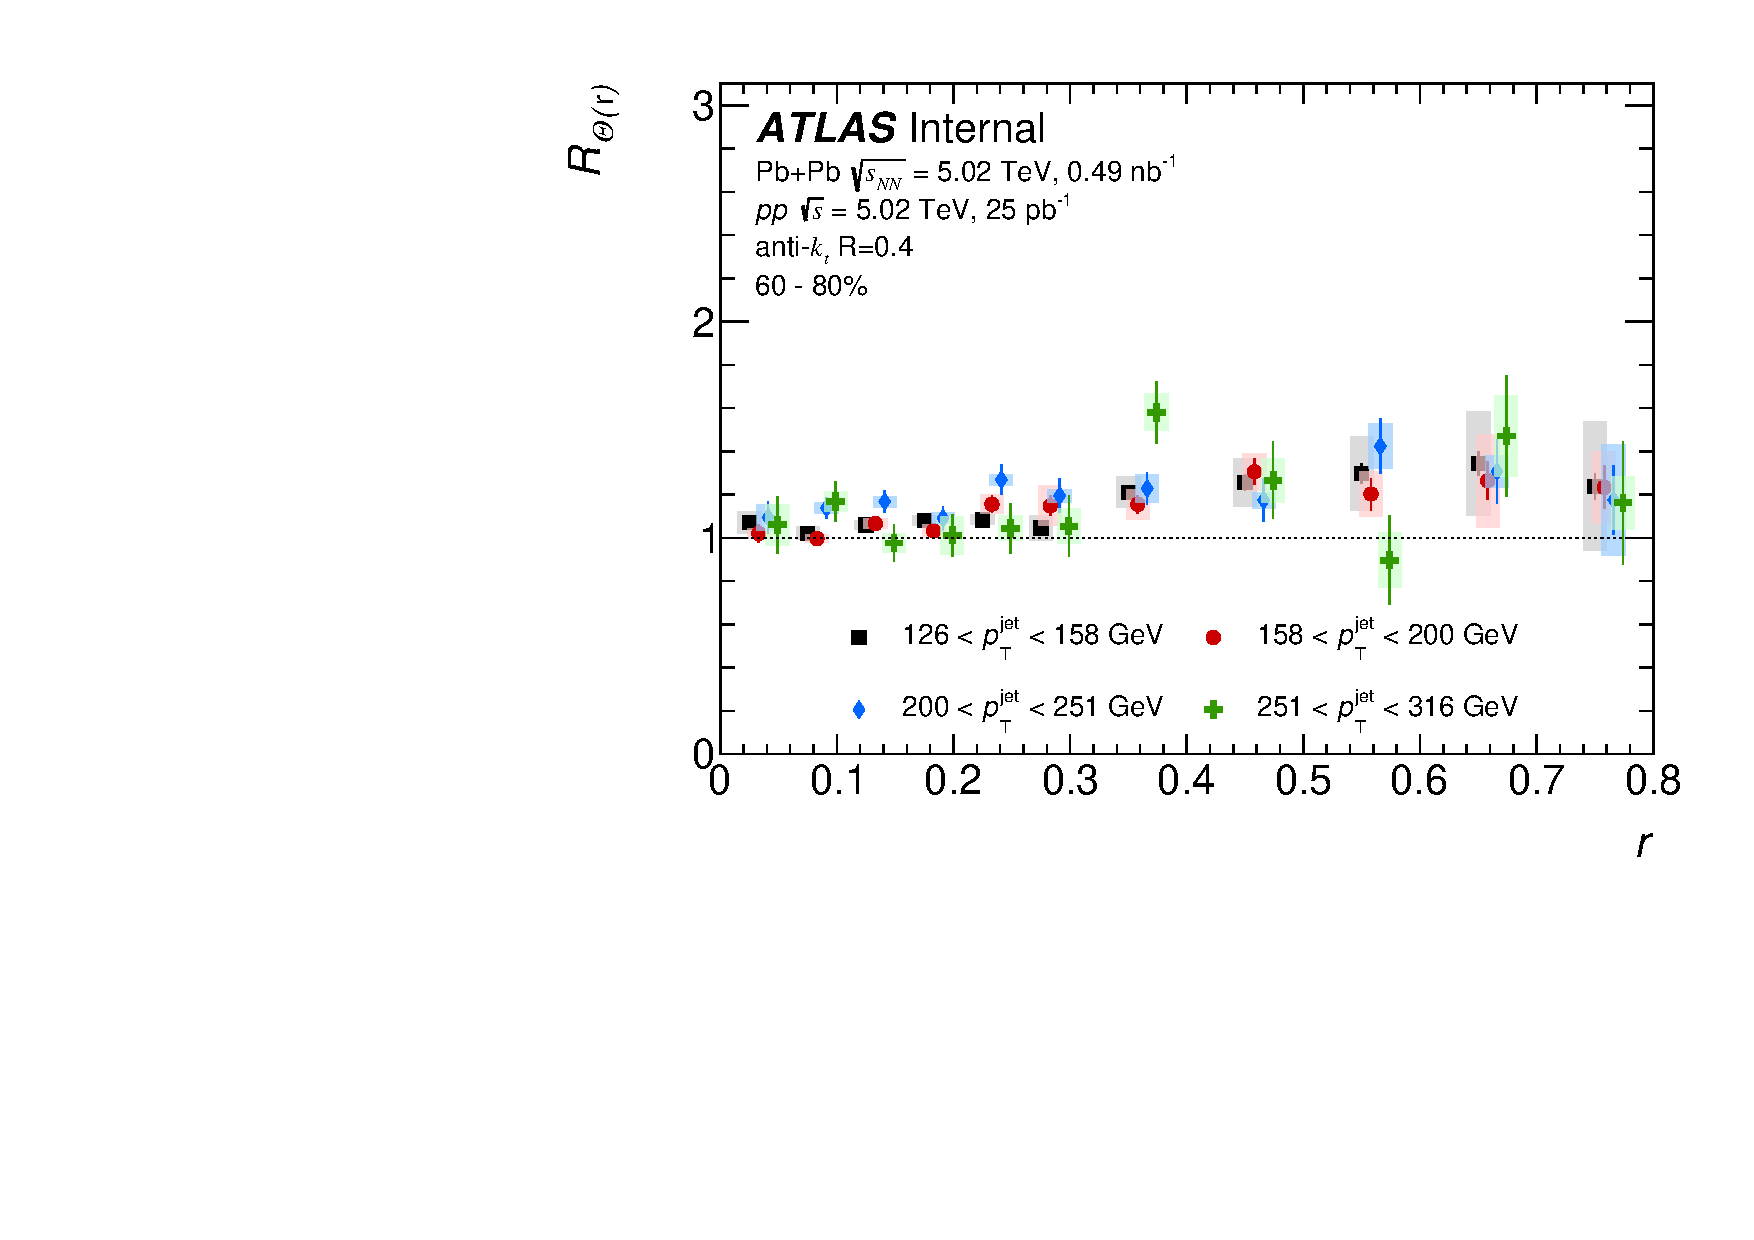
\includegraphics[width=0.5\textwidth]{figures/main/results/RDpT_lowpt_integ_cent5.pdf} &
	 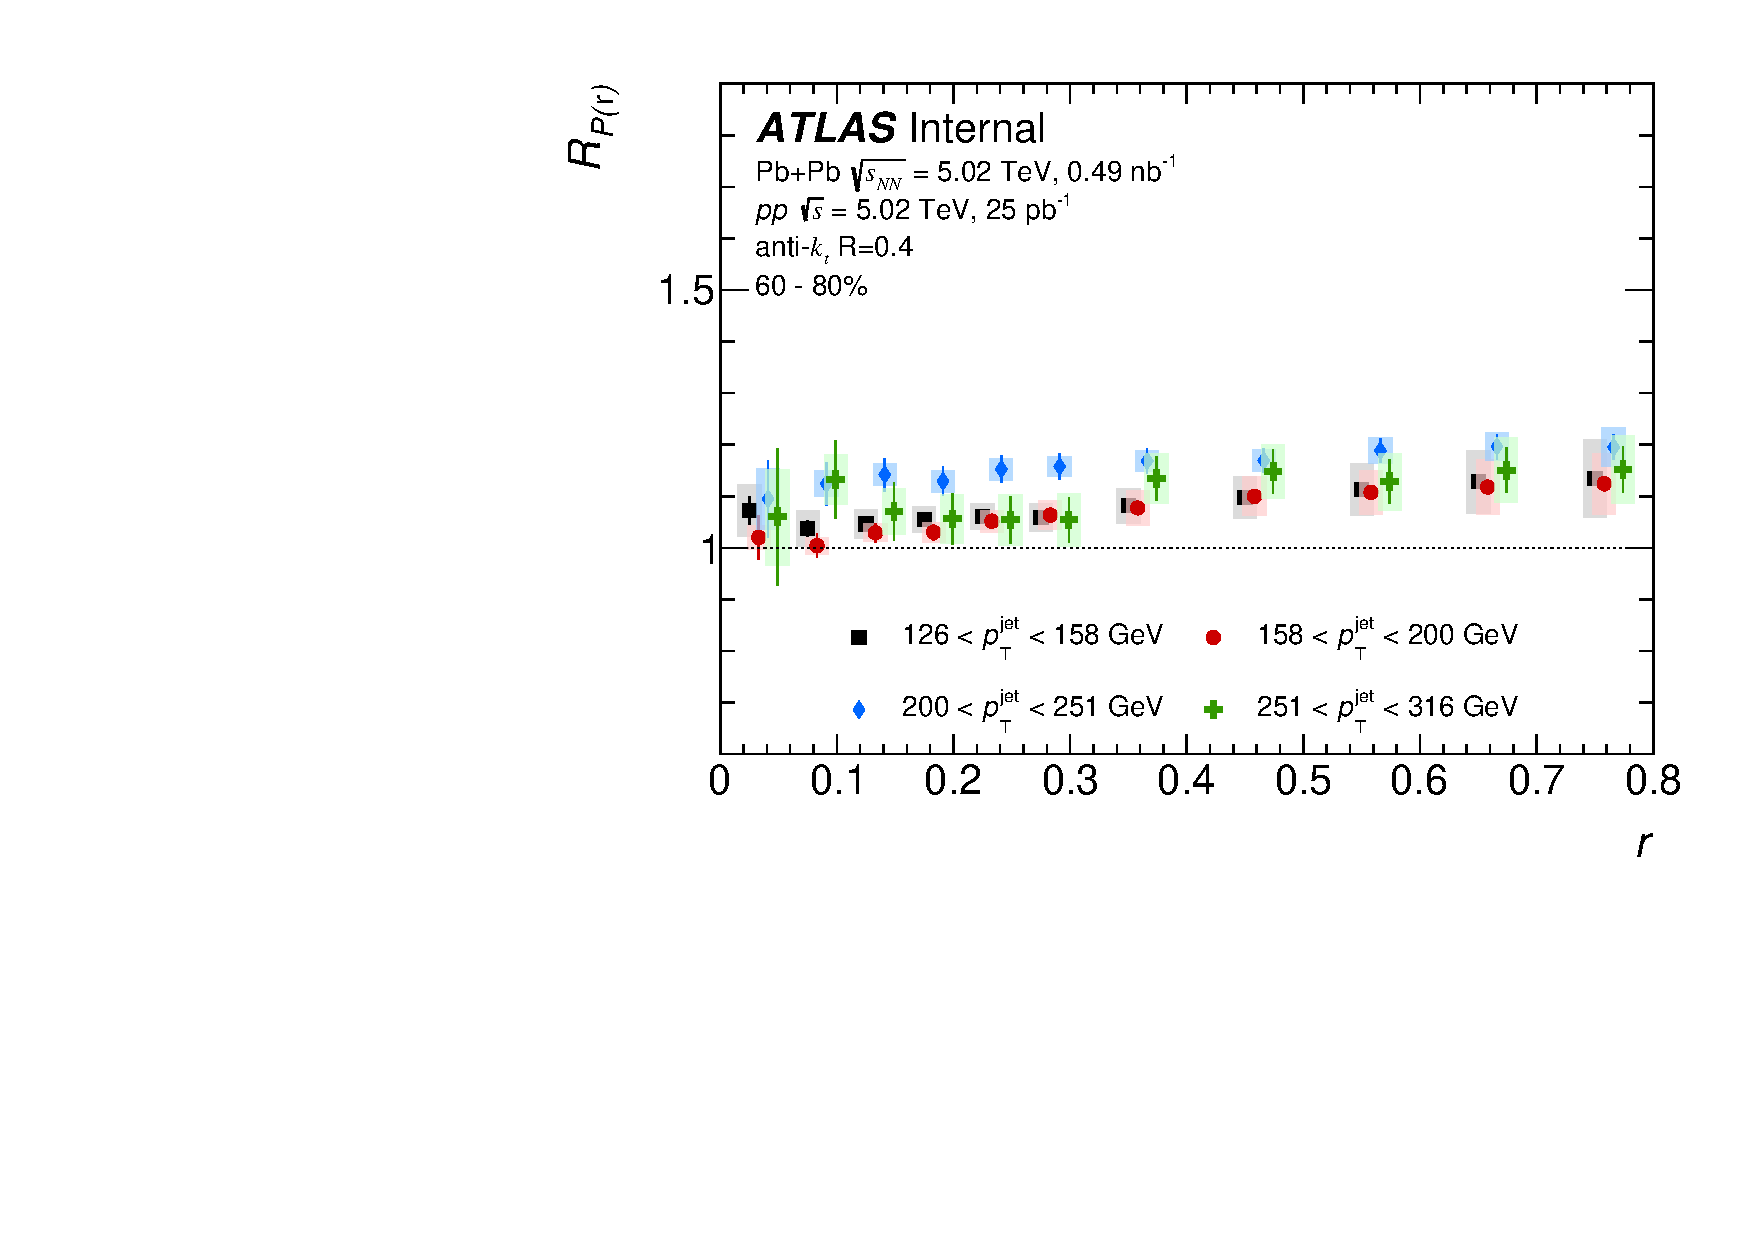
\includegraphics[width=0.5\textwidth]{figures/main/results/RDpT_jetshape_cent5.pdf} \\
\end{tabular} }
   \caption{\RTheta\ (left) and \RP\ (right) as a function of \rvar\ in central collisions for charged-particles with $\pt\ < 4$ GeV ranges in four \ptjet\ selections: 126--158~\GeV, 158--200~\GeV, 200--251~\GeV, and 251--316~\GeV and three centrality selections: 0--10\% (top), 30--40\% (middle) and 60--80\% (bottom).
The vertical bars on the data points indicate statistical uncertainties while the shaded boxes indicate systematic uncertainties.
The widths of the boxes are not indicative of the bin size and the points are shifted horizontally for better visibility.
}
      \label{fig:RPRT}
\end{figure}


Figure~\ref{fig:RPRT} shows \RTheta\ and \RP\ for 0--10\%, 30--40\% and 60--80\% central collisions.
 The \RTheta\ 
distributions of the most central collisions show a maximum for $\rvar \sim 0.4$ and decrease for larger \rvar.
However, since \RTheta\ remains at or above unity for the full range of \rvar\ values presented \RP\ continues
to slowly increase with increasing \rvar\ over the full measured range.
 In more peripheral collisions,
the magnitude of the excess is reduced and the trends in \RTheta\ are less clear, however the slow increase
of \RP\ is clearly seen for the 30--40\% central collisions.


%%%%%%%%%%%%%%%%%
%These measurements show that the excess of particles with $\pt <$~4.0~\GeV\ observed in~\cite{PhysRevC.98.024908} extends
%outside the \RFour\ jet cone.
%The measured dependence of \RDptr\ suggests that the energy lost by jets through the jet quenching process is being transferred to particles with $\pt <$~4.0~\GeV\ at larger radial distances from the jet axis.

%This is qualitatively consistent with theoretical calculations \mbox{\cite{Blaizot:2014ula}}.
%Additionally, these observations are in agreement with the previous measurement of jet fragmentation functions \cite{Chatrchyan:2014ava, Sirunyan:2018jqr, Aaboud:2017bzv, PhysRevC.98.024908} and may indicate the dependence of the response of the hot dense matter to the momentum of a jet passing through it.

%%%%%%%%%%%%%%%%%


\FloatBarrier
